% =========================================================================
%  MCAMS -- Monte Carlo Attenuation and Multiple Scattering
%  User manual
%  Compile with:   latexmk -pdf main.tex   (or: make)
%  or:             pdflatex main.tex  (three times, for the cross references)
%  Figures are produced by  python tools/make_figures.py
% =========================================================================
\documentclass[11pt,a4paper]{report}
% ======================================================================
% preamble.tex - packages, macros and styles of the MCAMS manual
% (same visual style as the pycorrect manual)
% ======================================================================
\usepackage[T1]{fontenc}
\usepackage[utf8]{inputenc}
\usepackage{mathpazo}
\renewcommand{\ttdefault}{txtt}   % txfonts typewriter: narrower than Courier
\usepackage{microtype}
% no ligatures in typewriter text: "--fullness" must not become an en-dash
\DisableLigatures[-]{encoding = T1, family = tt*}
\usepackage[english]{babel}
\usepackage[a4paper,margin=2.5cm,headheight=14pt]{geometry}
\usepackage{amsmath,amssymb}
\usepackage{graphicx}
\usepackage{booktabs,tabularx,longtable,array}
\usepackage{xcolor}
\usepackage{listings}
\usepackage[most]{tcolorbox}
\usepackage{enumitem}
\usepackage{fancyhdr}
\usepackage{titlesec}
\usepackage{caption}
\usepackage{float}
\usepackage{tikz}
\usetikzlibrary{arrows.meta,positioning,shapes.geometric}
\usepackage[colorlinks=true,linkcolor=accent,urlcolor=accent,citecolor=accent]{hyperref}

\graphicspath{{figures/}}
\setcounter{tocdepth}{1}
\emergencystretch=2em

% ---------------------------------------------------------------- colours
\definecolor{accent}{HTML}{2A78D6}
\definecolor{accent2}{HTML}{EB6834}
\definecolor{accent3}{HTML}{1BAF7A}
\definecolor{ink2}{HTML}{52514E}
\definecolor{codebg}{HTML}{F6F6F4}
\definecolor{outbg}{HTML}{EEF4FC}
\definecolor{noteback}{HTML}{EEF4FC}
\definecolor{warnback}{HTML}{FDF0EA}

% ---------------------------------------------------------------- headings
\titleformat{\chapter}[display]{\normalfont\bfseries\color{accent}}
  {\large\scshape \chaptertitlename\ \thechapter}{4pt}{\Huge}
\titlespacing*{\chapter}{0pt}{-20pt}{24pt}
\titleformat{\section}{\normalfont\Large\bfseries\color{accent}}{\thesection}{0.8em}{}
\titleformat{\subsection}{\normalfont\large\bfseries}{\thesubsection}{0.8em}{}

\pagestyle{fancy}
\fancyhf{}
\fancyhead[L]{\small\color{ink2}\textsc{mcams} user manual}
\fancyhead[R]{\small\color{ink2}\nouppercase{\leftmark}}
\fancyfoot[C]{\small\thepage}
\renewcommand{\headrulewidth}{0.4pt}

% ---------------------------------------------------------------- code
% Python code, program output and shell commands. The chapters use
%   \begin{lstlisting} ... \end{lstlisting}            (Python, default)
%   \begin{lstlisting}[style=shell] ... \end{lstlisting}
%   \pyexample{name}  (examples/name.py followed by examples/output/name.txt)
\lstdefinestyle{base}{
  basicstyle=\ttfamily\small, backgroundcolor=\color{codebg},
  frame=single, rulecolor=\color{codebg}, framesep=4pt, xleftmargin=4pt,
  xrightmargin=4pt, breaklines=true, columns=fullflexible, keepspaces=true,
  showstringspaces=false, aboveskip=8pt, belowskip=8pt,
  commentstyle=\color{ink2}\itshape, keywordstyle=\color{accent}\bfseries,
  stringstyle=\color{accent2}, upquote=true}
\lstdefinestyle{pycode}{style=base, language=Python}
\lstdefinestyle{shell}{style=base, language={}}
\lstdefinestyle{output}{style=base, language={}, basicstyle=\ttfamily\scriptsize,
  backgroundcolor=\color{outbg}, rulecolor=\color{outbg}, aboveskip=0pt}
\lstset{style=pycode}

\newcommand{\pyexample}[1]{%
  \lstinputlisting[style=pycode]{examples/#1.py}%
  \lstinputlisting[style=output]{examples/output/#1.txt}}

% \code{...}: typewriter text for names, calls and short pieces of code.
% Spaces, underscores and other special characters are allowed inside; braces
% must be balanced. Do not use it in titles or captions (use \texttt there).
\newcommand{\code}[1]{\texttt{\detokenize{#1}}}
\newcommand{\file}[1]{\texttt{#1}}

% ---------------------------------------------------------------- boxes
\newtcolorbox{note}[1][Note]{colback=noteback,colframe=accent,boxrule=0pt,
  leftrule=3pt,arc=0pt,fonttitle=\bfseries,coltitle=accent,colbacktitle=noteback,
  title=#1,attach title to upper={\ \ },before skip=8pt,after skip=8pt}
\newtcolorbox{warn}[1][Caution]{colback=warnback,colframe=accent2,boxrule=0pt,
  leftrule=3pt,arc=0pt,fonttitle=\bfseries,coltitle=accent2,colbacktitle=warnback,
  title=#1,attach title to upper={\ \ },before skip=8pt,after skip=8pt}
\newtcolorbox{fnbox}[1]{colback=white,colframe=accent,boxrule=0.6pt,arc=2pt,
  fonttitle=\ttfamily\bfseries,coltitle=white,title={#1},before skip=10pt,after skip=6pt}

\setlist{itemsep=2pt,topsep=4pt}
\captionsetup{font=small,labelfont={bf,color=accent}}
\setlength{\parindent}{0pt}
\setlength{\parskip}{5pt}

% ---------------------------------------------------------------- macros
\newcommand{\mcams}{\textsc{mcams}}
\newcommand{\twotheta}{2\theta}
\newcommand{\mumm}{\mu\ (\mathrm{mm}^{-1})}
\newcommand{\deriv}[1]{\mathrm{d}#1}
\DeclareMathOperator{\e}{e}


\begin{document}

% ---------------------------------------------------------------- title
\begin{titlepage}
\thispagestyle{empty}
\vspace*{2.5cm}
{\color{accent}\rule{\linewidth}{2pt}}\par\vspace{0.6cm}
{\fontsize{44}{48}\selectfont\bfseries\mcams}\par\vspace{0.3cm}
{\LARGE Monte Carlo Attenuation and Multiple Scattering}\par\vspace{0.2cm}
{\Large\color{ink2} Particle trajectories through layered slab, disc, cylindrical and
spherical samples, with layers of any vertical extent}\par
\vspace{0.6cm}{\color{accent}\rule{\linewidth}{2pt}}\par
\vspace{1.5cm}
{\Large User Manual}\par\vspace{0.3cm}
{\large Version 2.7 \quad(worked examples in the notation of \textsc{correct}; all the factors $A_{x,y}$)}\par
{\normalsize\color{ink2} The Python modules are those of version 2.4}\par
\vfill
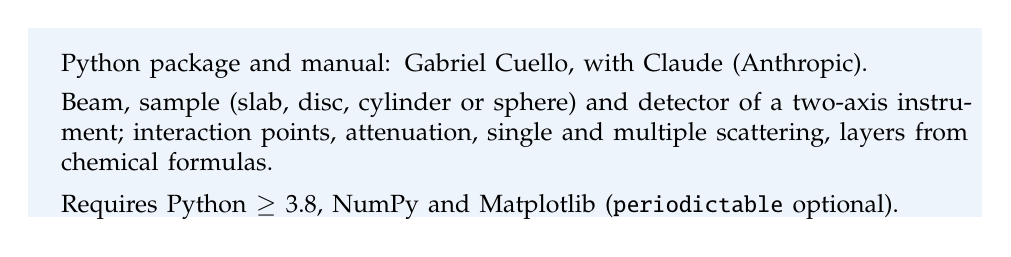
\begin{tikzpicture}
  \fill[noteback] (0,0) rectangle (\linewidth,2.4);
  \node[anchor=north west,text width=0.95\linewidth,align=left] at (0.3,2.2) {
  \small Python package and manual: Gabriel Cuello, with Claude (Anthropic).\\[3pt]
  Beam, sample (slab, disc, cylinder or sphere) and detector of a two-axis instrument; interaction points,
  attenuation, single and multiple scattering, layers from chemical formulas.\\[3pt]
  Requires Python $\geq$ 3.8, NumPy and Matplotlib (\texttt{periodictable} optional).};
\end{tikzpicture}
\vspace{1cm}
{\small\color{ink2}\today}
\end{titlepage}

\pagenumbering{roman}
\tableofcontents
\clearpage
\pagenumbering{arabic}

\chapter{Introduction}
\label{ch:intro}

\section{What \mcams\ does}

\mcams\ (Monte Carlo Attenuation and Multiple Scattering) is a Python package that simulates, with the Monte Carlo method, what happens to particles
(for example neutrons or X-ray photons) of a rectangular beam that crosses a
sample and is detected at a scattering angle $2\theta$. The sample is made of
layers, each one with its own material. Four geometries are available:
\begin{itemize}
  \item a \textbf{slab}: flat rectangular layers stacked one behind the other, which can be rotated
        around the vertical axis with respect to the beam;
  \item a \textbf{disc}: the same, but with a circular section centred on the beam, as a round flat cell or a pellet
        (version 2.3, Chapter~\ref{ch:disc});
  \item a \textbf{sphere}: concentric spheres (a full sphere surrounded by spherical shells) centred on the beam
        (version 2.4, Chapter~\ref{ch:sphere});
  \item a \textbf{cylinder}: concentric cylinders (a full inner cylinder surrounded by
        annular layers) with a vertical axis at the centre of the instrument.
\end{itemize}
In all the geometries every layer has its own \textbf{vertical extent}: its material lies between a bottom and a
top, measured from the centre of the beam, and the layer is empty below and above. This describes a container
that is not full, a powder resting on a support, or a container that starts inside the beam. Part of the beam
can then pass over or under the material (Chapter~\ref{ch:partial}).
The detector is the one of a two-axis instrument: it moves on a circle centred on
the sample, in the horizontal plane (Figure~\ref{fig:instrument}).

With the package you can answer questions such as:
\begin{enumerate}
  \item Where in the beam does each particle start? (Chapter~\ref{ch:beam})
  \item In which layer, and at which point, does a particle interact? (Chapters~\ref{ch:sample} and~\ref{ch:physics})
  \item What fraction of the scattered particles leaves the sample towards the detector,
        as a function of the angle? (Chapter~\ref{ch:transmission})
  \item How many particles reach the angle $2\theta$ after exactly one scattering, and how many
        after two or more? (Chapter~\ref{ch:scattering})
  \item How does that transmission depend on the layer in which the \emph{last} scattering
        happened? (Chapter~\ref{ch:lastlayer})
  \item Which are the attenuation coefficient and the scattering ratio of a layer, given its
        chemical formula, density and cross sections? (Chapter~\ref{ch:builder})
  \item How do all these results change when the container is only partially filled, or when the
        material does not start at the bottom of the beam? (Chapter~\ref{ch:partial})
  \item How does a round flat sample differ from a rectangular one? (Chapter~\ref{ch:disc})
  \item How does a spherical sample differ from a cylindrical one? (Chapter~\ref{ch:sphere})
  \item How do I compute the attenuation factors and the multiple scattering of a sample in a container inside a furnace, as
        \textsc{correct} does, but with the Monte Carlo? (Chapter~\ref{ch:correct})
  \item Which are the exact single-scattering attenuation factors of each layer, to use as a reference
        for the Monte Carlo? (Chapter~\ref{ch:direct})
\end{enumerate}

\begin{note}[New in version 2.0]
Layers of different heights, aligned on the bottom of the sample: each layer has a fill height, or a
\emph{fullness} (the fraction of the beam height covered by its material). The samples of earlier versions,
with all layers full, give the same numbers as before.
\end{note}

\begin{note}[New in version 2.1]
The \emph{direct method} (module \code{direct_attenuation.py}, Chapter~\ref{ch:direct}): single-scattering attenuation factors
(Paalman \& Pings factors) of every layer computed with exact weights instead of random interactions. It is a precise reference for the
Monte Carlo, and much faster for containers and weakly attenuating layers.
\end{note}

\begin{note}[New in version 2.7 of the manual]
The worked examples of Chapter~\ref{ch:correct} and the comparison sphere/cylinder of Chapter~\ref{ch:sphere} are computed on fine
angular grids: attenuation factors every $1^\circ$, multiple scattering every $2^\circ$ (Section~\ref{sec:grid}). The package is unchanged.
\end{note}

\begin{note}[New in version 2.6 of the manual]
All the 21 attenuation factors $A_{x,y}$ ($x$ = s, c, h; $y$ = s, c, h, sc, sh, ch, sch), what each one is for, and a general correction
by least squares with any set of measured runs (Section~\ref{sec:all-factors}, Example~18). The package is unchanged.
\end{note}

\begin{note}[New in version 2.5 of the manual]
A chapter of worked examples (Chapter~\ref{ch:correct}): the attenuation factors $A_{s,sch}$, $A_{c,sch}$, $A_{h,sch}$, $A_{c,ch}$,
$A_{h,ch}$, $A_{h,h}$ in the notation of \textsc{correct}, and the single, multiple and total scattering of the three runs $I_{sch}$,
$I_{ch}$, $I_h$, for a cylinder, an annular sample, a slab, a disc and a sphere, each in a container inside a furnace. The package is
unchanged (the modules are those of version 2.4); a helper file, \file{correct\_tools.py}, is provided with the examples.
\end{note}

\begin{note}[New in version 2.4]
The \emph{sphere} geometry (module \code{sphere.py}, Chapter~\ref{ch:sphere}): concentric spheres centred on the beam, given from the
inner one outwards as the cylinders (the first thickness is the diameter). Its layers have the same properties as those of the other
geometries, partial filling included. The results of the other geometries are exactly those of version 2.3.
\end{note}

\begin{note}[New in version 2.3]
The \emph{disc} geometry (module \code{disc.py}, Chapter~\ref{ch:disc}): a flat sample with a circular section, made of layers stacked
along its normal, centred on the beam and rotatable like the slab. Its layers have the same properties as those of the other
geometries, partial filling included. The results of the slab and the cylinder are exactly those of version 2.2.
\end{note}

\begin{note}[New in version 2.2]
The bottom of each layer is free: a layer is described by its \code{bottom} and \code{height}, in mm from the centre
of the beam (Chapter~\ref{ch:partial}). The sample height can be left out (the envelope of the layers is used), and
the fullness of every layer is given as a result, \code{sample.beam_fullness()}. The forms of version 2.0 are still
accepted, and the samples of earlier versions give the same numbers as before.
\end{note}

\section{Design principles}

\begin{itemize}
  \item \textbf{Simple routines.} The code is a collection of short functions, classes and methods,
        each one doing one thing. Every module starts with an explanation of what it does and with a
        short glossary of the NumPy functions that it uses, and the code is commented step by step,
        so that it can be read as a tutorial.
  \item \textbf{One interface, four geometries.} Slab, disc, cylinder and sphere implement the same methods
        (Chapter~\ref{ch:sample}). The analysis modules only use that interface, so every
        calculation works with all of them, and new geometries can be added. The disc and the sphere show how: the
        disc is a slab whose section is a circle (Chapter~\ref{ch:disc}), the sphere a cylinder whose surfaces are
        spheres (Chapter~\ref{ch:sphere}).
  \item \textbf{Vectorised.} Thousands of particles are processed at once with NumPy arrays; there
        are no Python loops over particles.
  \item \textbf{Units.} All distances are in millimetres, linear attenuation coefficients in
        mm$^{-1}$, angles in degrees (the user side) and cross sections in barn.
  \item \textbf{Reproducible.} Every random calculation accepts \code{rng=} (a seed or a NumPy
        random generator), so the results can be repeated exactly.
\end{itemize}

\section{The modules}

\begin{figure}[ht]
  \centering
  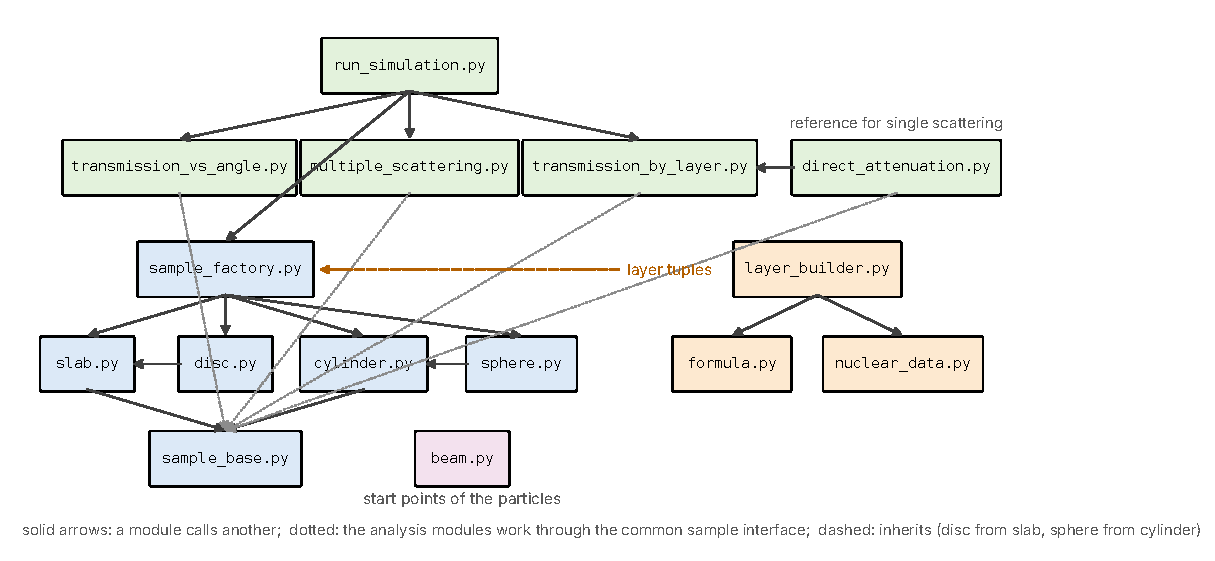
\includegraphics[width=0.95\textwidth]{fig_modules}
  \caption{The modules of the package and how they depend on each other. The
  analysis modules (green) work with any sample (blue) through the common interface
  defined in \texttt{sample\_base.py}; the modules in orange prepare the data of the layers.}
  \label{fig:modules}
\end{figure}

\begin{table}[ht]
  \centering\small
  \begin{tabular}{@{}p{4.6cm}p{10.2cm}@{}}
    \toprule
    \textbf{File} & \textbf{Content} \\ \midrule
    \code{beam.py}                 & Random start points of the particles in a rectangular beam, with optional profiles $H(x)$ and $V(y)$. \\
    \code{sample_base.py}          & The \code{Layer} record (with its filling), the abstract class \code{LayeredSample} (the common interface, vertical extent and filling of the layers) and \code{scattered_direction}. \\
    \code{slab.py}                 & Slab geometry: \code{SlabSample} and \code{create_slab_sample}. \\
    \code{disc.py}                 & Disc geometry (version 2.3): \code{DiscSample} (a \code{SlabSample} with a circular section) and \code{create_disc_sample}. \\
    \code{sphere.py}               & Sphere geometry (version 2.4): \code{SphericalSample} (a \code{CylindricalSample} with spherical surfaces) and \code{create_spherical_sample}. \\
    \code{cylinder.py}             & Cylindrical geometry: \code{CylindricalSample} and \code{create_cylindrical_sample}. \\
    \code{sample_factory.py}       & \code{make_sample}: builds a slab, a disc, a cylinder or a sphere from a name. \\
    \code{transmission_vs_angle.py}& Transmission of the scattered particles versus $2\theta$. \\
    \code{multiple_scattering.py}  & Particle-by-particle simulation: single and multiple scattering versus $2\theta$. \\
    \code{transmission_by_layer.py}& Transmission versus $2\theta$, one curve per layer of last scattering. \\
    \code{direct_attenuation.py}  & Direct method: single-scattering attenuation factors with exact weights, the same from the Monte Carlo, comparison. \\
    \code{formula.py}              & Reader of chemical formulas, with isotopes. \\
    \code{nuclear_data.py}         & Atomic masses and (optional) tabulated neutron cross sections. \\
    \code{layer_builder.py}        & Computes $\mu$ and the scatter fraction of a layer from formula, density and cross sections. \\
    \code{run_simulation.py}       & Main script: chooses the geometry and runs the whole chain. \\ \bottomrule
  \end{tabular}
  \caption{Files of the package.}
  \label{tab:files}
\end{table}

\section{A first look}

Everything below can be run from the folder that contains the modules. The quickest way to see
the package at work is the main script (Chapter~\ref{ch:main}), which builds an example sample,
computes the three kinds of results and saves the plots:
\begin{lstlisting}[style=shell]
python run_simulation.py --geometry slab
python run_simulation.py --geometry cylinder
python run_simulation.py --geometry cylinder --fullness 0.5
python run_simulation.py --geometry cylinder --bottom -6 --height 5
python run_simulation.py --geometry disc --plane-angle 45
python run_simulation.py --geometry sphere
\end{lstlisting}
From Python, the same chain is available as a function:
\begin{lstlisting}
from run_simulation import run_simulation
results = run_simulation("cylinder", n_particles=200000, show=False)
\end{lstlisting}
The rest of the manual explains each step separately.

\section{Notation used in this manual}

Names of files, functions and variables are written in \code{typewriter}. Mathematical symbols are listed
in Appendix~\ref{app:symbols}. Results shown as examples were obtained with the example samples of the
main script: they are illustrative, and the layer data (attenuation coefficients and scatter fractions)
are not those of a real experiment.

\chapter{Installation and requirements}
\label{ch:install}

\section{Requirements}

\begin{itemize}
  \item \textbf{Python} 3.8 or newer (the package was developed and tested with Python 3.12).
  \item \textbf{NumPy} (tested with 2.4) for all the calculations.
  \item \textbf{Matplotlib} (tested with 3.10) for the plots. It is only needed by the \code{plot_...}
        functions and by the demonstrations at the end of the modules.
  \item \textbf{periodictable} (optional): tabulated neutron cross sections and atomic masses for
        Chapter~\ref{ch:builder}. Without it you provide the cross sections yourself.
\end{itemize}
To install what is needed:
\begin{lstlisting}[style=shell]
pip install numpy matplotlib
pip install periodictable        # optional
\end{lstlisting}

\section{Files and folders}

The package is a set of ordinary Python files that must be in the same folder (the \emph{code folder}).
There is nothing to install: the modules are found because they are in the folder from which you run Python
or the notebook.
\begin{lstlisting}[style=shell]
code folder/
    beam.py  sample_base.py  slab.py  disc.py  cylinder.py  sphere.py  sample_factory.py
    transmission_vs_angle.py  multiple_scattering.py  transmission_by_layer.py
    direct_attenuation.py  formula.py  nuclear_data.py  layer_builder.py  run_simulation.py
    tests/test_mcams.py         (self-test)
    manual/                     (this manual)
\end{lstlisting}

\section{Checking the installation}

Every module has a short demonstration at its end, which runs when the file is executed. From the code folder:
\begin{lstlisting}[style=shell]
python slab.py          # flat cell, partially filled: interaction points and paths
python cylinder.py      # can, partially filled: the same
python disc.py          # round cell, partially filled; beam larger than the disc
python sphere.py        # spherical container half filled with a powder
python formula.py       # chemical formulas
python layer_builder.py # layers from formulas
\end{lstlisting}
If these run without errors, the package is ready. The folder \file{tests/} contains a self-test of the
geometry, which compares the paths with a brute-force calculation and the interaction rates with exact results:
\begin{lstlisting}[style=shell]
python tests/test_mcams.py
...
ALL PASSED
\end{lstlisting}

\section{Use in a Jupyter notebook}

Two points deserve attention in notebooks:
\begin{enumerate}
  \item Python imports a module only once per session. If you replace a file by a newer version, the notebook
        keeps using the old one until the \textbf{kernel is restarted} (or the module is reloaded with
        \code{importlib.reload}). A message such as \code{TypeError: create_slab_sample() got an unexpected keyword argument ...}
        usually means that an old version is still loaded (see Appendix~\ref{app:trouble}).
  \item Cells of a notebook can be run in any order. After changing the sample or the beam, run again the cells that depend on them.
\end{enumerate}

\section{Reproducibility}

All the functions that use random numbers accept the argument \code{rng}, which can be an integer
(a seed) or a NumPy generator created with \code{np.random.default_rng(seed)}. With the same seed the
results are identical from one run to the next. Without it, every run gives slightly different
results, as expected from a Monte Carlo method.

\chapter{Geometry and conventions}
\label{ch:geometry}

\section{Frames of reference and units}

Two frames are used.
\begin{description}
  \item[Lab frame.] The $z$ axis is the direction of the incident beam, $x$ is horizontal
        and $y$ is vertical. The origin is the centre of rotation of the instrument, that is, the centre of the circle
        on which the detector moves. All the data given by the user (beam, detector angle, directions) are in this frame.
  \item[Sample frame.] A frame attached to the sample, in which its geometry is simplest. For a slab,
        or a disc, $z'$ is the normal of the layers; for a vertical cylinder and for a sphere it coincides with the lab frame. The
        samples convert between the two with \code{to_sample_frame} and \code{to_lab_frame}.
\end{description}
All lengths are in millimetres; linear attenuation coefficients are in mm$^{-1}$.

\section{The instrument}

The detector of a two-axis instrument moves on a circle in the horizontal plane $y=0$, centred on the sample
(Figure~\ref{fig:instrument}). The scattering angle $\twotheta$ is the angle between the direction of the
scattered particle and the direction of the incident beam ($+z$). It is measured from $+z$ towards $+x$, and
runs from $0^\circ$ (forward) to $180^\circ$ (backward).

\begin{figure}[ht]
  \centering
  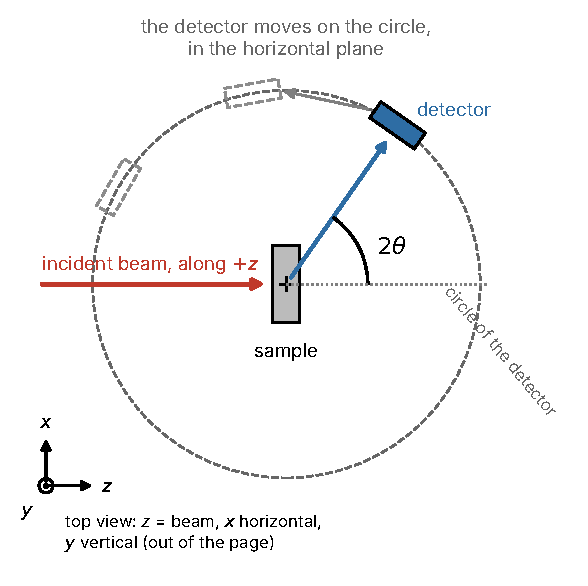
\includegraphics[width=0.78\textwidth]{fig_instrument}
  \caption{Top view of the instrument. The beam travels along $+z$ and hits the sample at the centre of the circle
  of the detector; the angle $\twotheta$ is measured between the incident direction and the direction of the detector.}
  \label{fig:instrument}
\end{figure}

A direction in space is given by two angles, the polar angle $\twotheta$ (from the beam) and the azimuth
$\varphi$ (around the beam, from $+x$ towards $+y$):
\begin{equation}
  \hat{d} = (\sin\twotheta\cos\varphi,\; \sin\twotheta\sin\varphi,\; \cos\twotheta).
\end{equation}
A detector in the horizontal plane has $\varphi=0$ (towards $+x$) or $\varphi=180^\circ$ (towards $-x$). This is
what the function \code{scattered_direction(two_theta_deg, phi_deg=0.0)} returns.

\section{The beam}

The beam is a rectangle of width $w_b$ (along $x$) and height $h_b$ (along $y$), centred on the beam axis and
perpendicular to $z$. Its intensity is described by two independent profiles, $H(x)$ and $V(y)$ (Chapter~\ref{ch:beam}).
A particle is identified by the point $(x,y)$ where it starts, in the plane perpendicular to the beam that contains
the origin.

\section{Vertical position of the sample}

Slab and cylinder have a height and a bottom, $y_\mathrm{bottom}$ (argument \code{y_bottom}). By default the sample is
centred on the beam: $y_\mathrm{bottom}=-\text{height}/2$, and it extends to $y_\mathrm{top}=y_\mathrm{bottom}+\text{height}$.
The disc and the sphere are always centred on the beam: they go from $-R$ to $+R$. In every geometry the material of a layer can occupy
only a band of heights, from its own bottom to its own top (Chapter~\ref{ch:partial}).

\section{The slab geometry}

The slab is a stack of flat layers (Figure~\ref{fig:slab}). Its section is a rectangle of width $w$ (horizontal)
and height $h$ (vertical), centred on the beam horizontally and, by default, vertically. The layers are given \emph{from the front face to the back}, each one with
its thickness along the normal $z'$.

The orientation is set by the \textbf{plane angle} $\alpha$ (\code{plane_angle_deg}): the angle between the incident beam
and the plane of the sample.
\begin{itemize}
  \item $\alpha=90^\circ$ (default): the plane is perpendicular to the beam (normal incidence); the sample frame and the lab
        frame coincide.
  \item $\alpha<90^\circ$: the sample is rotated around the vertical axis and its normal is tilted towards $+x$ by
        $\omega = 90^\circ-\alpha$. For $\alpha>90^\circ$ it is tilted towards $-x$.
  \item Values of $\alpha$ very close to $0^\circ$ or $180^\circ$ (beam parallel to the plane) are not allowed.
\end{itemize}
The axis of rotation is the vertical line through the centre of the front face, which lies on the beam axis.

\begin{figure}[ht]
  \centering
  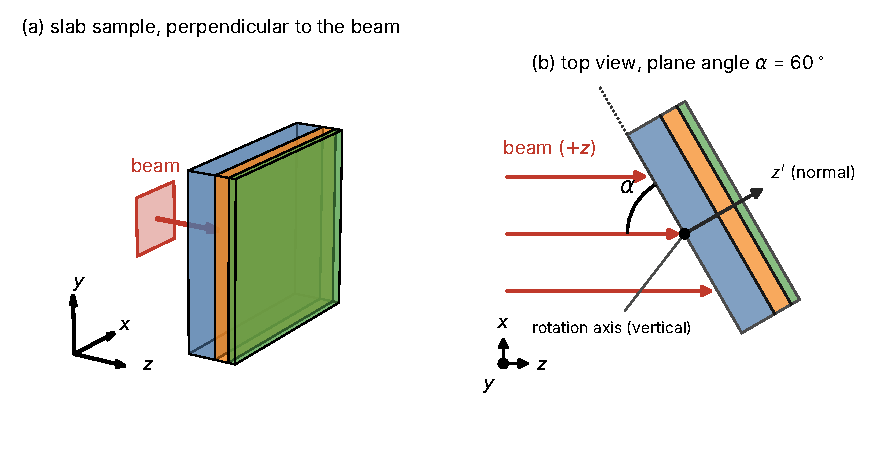
\includegraphics[width=\textwidth]{fig_slab_geometry}
  \caption{Slab geometry. (a)~Perspective view of a three-layer slab perpendicular to the beam; the red rectangle is the beam.
  (b)~Top view of the same sample rotated so that the angle between the beam and the plane of the sample is
  $\alpha=60^\circ$; $z'$ is the normal of the layers.}
  \label{fig:slab}
\end{figure}

\section{The disc geometry}

The disc (version 2.3) is a slab with a circular section: layers stacked along the normal $z'$, all with the same diameter
$D$, centred on the beam axis, and rotated around the vertical axis with the same plane angle $\alpha$ as the slab. It is
described in Chapter~\ref{ch:disc} (Figure~\ref{fig:disc}).

\section{The cylindrical geometry}

The sample is a set of concentric cylinders whose common axis is vertical and passes through the centre of the
instrument (Figure~\ref{fig:cylinder}). All the cylinders have the same height. The layers are given \textbf{from the
inner one outwards}:
\begin{itemize}
  \item the first layer is a full cylinder and its ``thickness'' is its \textbf{diameter}, so its radius is $r_1 = t_1/2$;
  \item the following layers are annuli and their thickness is the radial thickness: $r_k = r_{k-1} + t_k$.
\end{itemize}
For instance, the thicknesses $(6.0,\,1.0,\,0.5)$~mm give the radii $(3.0,\,4.0,\,4.5)$~mm and an outer diameter of 9~mm.
Because the cylinder is symmetric around its axis there is no orientation parameter. Particles can leave the sample through
the side surface and through the flat ends. All the cylinders start at the same bottom; each of them can be filled only up to
a given level (Chapter~\ref{ch:partial}).

\begin{figure}[ht]
  \centering
  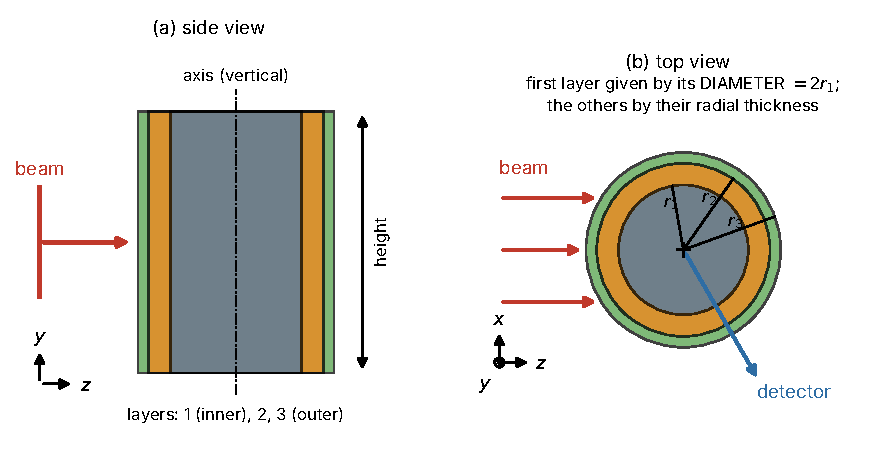
\includegraphics[width=\textwidth]{fig_cylinder_geometry}
  \caption{Cylindrical geometry. (a)~Side view: concentric cylinders of the same height, vertical axis. (b)~Top view:
  the radii $r_1<r_2<r_3$; the thickness of the first layer is its diameter $2r_1$.}
  \label{fig:cylinder}
\end{figure}

\section{The spherical geometry}

The sphere (version 2.4) is a set of concentric spheres centred on the beam axis, at the centre of the instrument. As for the
cylinder, the layers are given from the inner one outwards: the thickness of the first is its diameter, the others are radial
thicknesses. There is no orientation parameter. It is described in Chapter~\ref{ch:sphere} (Figure~\ref{fig:sphere}).

\section{Example trajectories}

Figure~\ref{fig:traj} shows, in top view, a few particles in both geometries: they enter along $+z$, interact at the
points marked with the colour of the layer in which they happen, and are then followed in the direction of a detector
at $\twotheta=100^\circ$ until they leave the sample. These are the paths that the package computes for thousands of
particles at once.

\begin{figure}[ht]
  \centering
  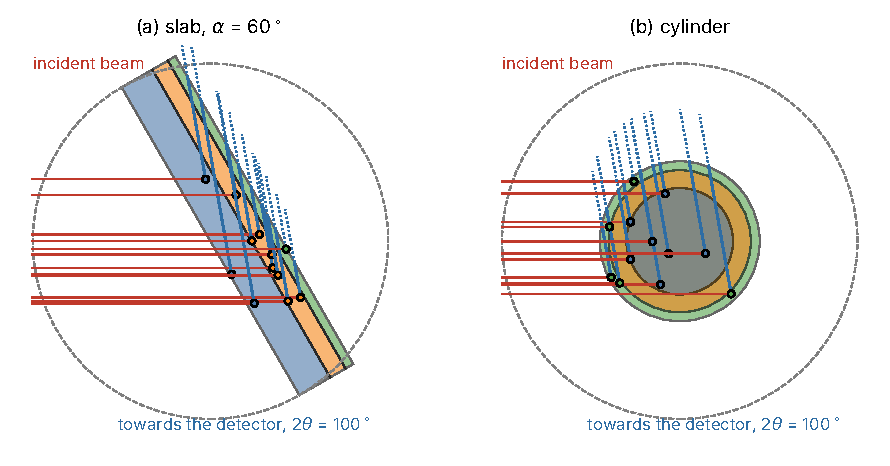
\includegraphics[width=\textwidth]{fig_trajectories}
  \caption{Examples of trajectories. Red: incident particles. Dots: interaction points, coloured by layer.
  Blue: path from the interaction point to the exit of the sample towards the detector ($\twotheta=100^\circ$); the dotted
  continuation only shows the direction. (a)~Slab with $\alpha=60^\circ$. (b)~Cylinder.}
  \label{fig:traj}
\end{figure}

\chapter{The incident beam}
\label{ch:beam}

\section{What it does}

The module \code{beam.py} chooses the point $(x,y)$ of the beam rectangle where each particle starts. Its main
function is
\begin{lstlisting}
sample_beam_point(width, height, H=None, V=None, n=1, rng=None)
\end{lstlisting}
\begin{description}
  \item[\code{width}, \code{height}] size of the beam along $x$ and $y$, in mm.
  \item[\code{H}, \code{V}] optional functions $H(x)$ and $V(y)$ (with $x$ and $y$ in mm) giving the relative intensity
        across the beam. They need not be normalised; they must be non-negative. By default both are uniform.
  \item[\code{n}] number of particles. With \code{n=1} the result is a pair of numbers; otherwise a pair of arrays.
  \item[\code{rng}] seed or random generator.
\end{description}
The result is the start point in mm, relative to the centre of the beam: $x\in[-w_b/2,\,w_b/2]$ and
$y\in[-h_b/2,\,h_b/2]$. The two profiles are treated as independent, so the intensity map is $H(x)\,V(y)$.
The function \code{start_position} returns the same point as a three-dimensional position together with the direction
of flight $(0,0,1)$.

\section{Method: inverse transform sampling}

For a uniform profile, the position is a uniform random number in the interval. For any other profile the
function uses \emph{inverse transform sampling}. The profile $f(x)$ is evaluated on a fine grid, and its cumulative
distribution
\begin{equation}
  F(x) = \frac{\int_{-w_b/2}^{x} f(x')\,\deriv{x'}}{\int_{-w_b/2}^{w_b/2} f(x')\,\deriv{x'}}
\end{equation}
is computed with the trapezoidal rule. If $u$ is a random number uniform between 0 and 1, then $x=F^{-1}(u)$ is distributed
according to $f$: where the profile is high $F$ grows fast, so many values of $u$ are mapped to that region. The inverse is
read with \code{np.interp}. This method needs neither the maximum of the profile nor rejected points.

\section{Example}

\pyexample{ex01_beam}

Figure~\ref{fig:beam} shows 6000 start points of a $10\times6$~mm beam with a Gaussian horizontal profile
($\sigma=1.5$~mm) and a uniform vertical profile.

\begin{figure}[ht]
  \centering
  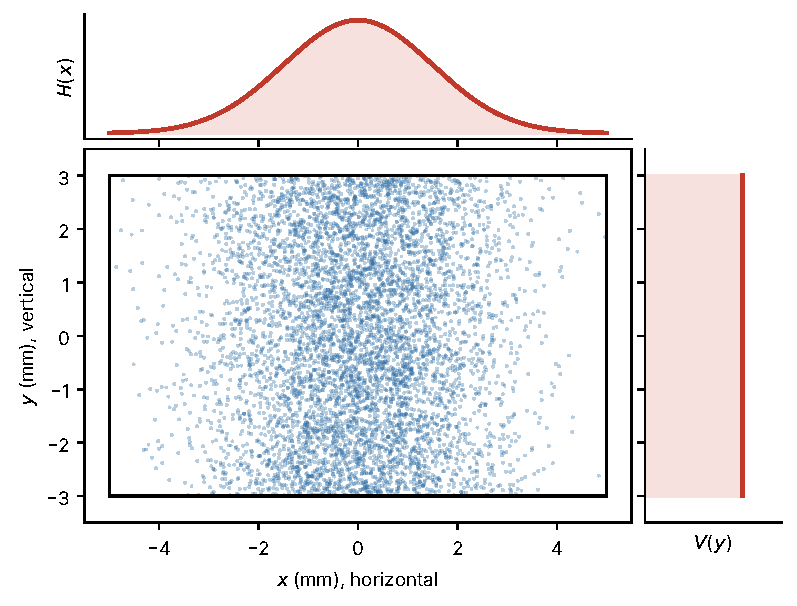
\includegraphics[width=0.75\textwidth]{fig_beam}
  \caption{Start points of the particles in a beam $10\times6$~mm with a Gaussian $H(x)$ ($\sigma=1.5$~mm) and a uniform $V(y)$.
  The curves are the profiles.}
  \label{fig:beam}
\end{figure}

A profile can be any function that accepts a NumPy array, for instance a measured profile interpolated with
\code{np.interp}:
\begin{lstlisting}
x_measured = np.array([-4, -2, 0, 2, 4]);  I_measured = np.array([0, 0.5, 1, 0.5, 0])
H = lambda x: np.interp(x, x_measured, I_measured)
xs, ys = sample_beam_point(8, 6, H=H, n=10000)
\end{lstlisting}
If a profile only accepts single numbers, the function calls it once per grid point.

\chapter{Describing the sample}
\label{ch:sample}

\section{The layer}

Every layer is described by four values and, optionally, its vertical extent, grouped in the record \code{Layer} (module \code{sample_base.py}):
\begin{center}
\begin{tabular}{@{}lp{10.5cm}@{}}
  \toprule
  \textbf{Field} & \textbf{Meaning} \\ \midrule
  \code{name} & Label of the material (free text, e.g. \code{"Fe"}). \\
  \code{thickness} & Size of the layer in mm, $>0$. Slab: along the normal. Cylinder: radial thickness, except for the first layer, for which it is the \emph{diameter}. \\
  \code{mu} & Total linear attenuation coefficient in mm$^{-1}$ (scattering + absorption), $\ge 0$. Use 0 for a gap. \\
  \code{scatter_fraction} & Fraction of the interactions that are scattering (the rest is absorption), between 0 and 1. Default 1. Only needed for multiple scattering. \\
  \code{bottom} & Optional (version 2.2). Height $y$ of the bottom of the material, in mm from the centre of the beam. Default \code{None}: the bottom of the sample. \\
  \code{height} & Optional (version 2.2). Height of the material in mm; the layer is empty below \code{bottom} and above \code{bottom + height}. Default \code{None}: up to the top of the sample. \\
  \code{fill_height} & Optional (version 2.0), instead of \code{bottom}/\code{height}: height of the material in mm above the bottom of the sample. \\
  \code{fullness} & Optional (version 2.0), instead of \code{bottom}/\code{height}: fraction of the beam height covered by the material, starting at the bottom of the sample (1 = full). Needs the \code{beam_height} of the sample. \\ \bottomrule
\end{tabular}
\end{center}
In practice a layer is written as a plain tuple \code{(name, thickness, mu, scatter_fraction)}; the last element is optional, and a
fifth element gives the fill height. A \code{Layer} object or a dictionary with the same field names can be used as well;
they are needed to give \code{bottom} and \code{height} (Chapter~\ref{ch:partial}). The function \code{make_layer_tuple} of Chapter~\ref{ch:builder} computes such a tuple from the chemical
formula and the density.

\section{Creating a sample}

\begin{description}[style=unboxed,leftmargin=0pt]
  \item[\code{create_slab_sample(width, height, layers, z_front=0.0, plane_angle_deg=90.0, y_bottom=None, beam_height=None)}]
        slab of section \code{width}$\times$\code{height} mm; layers from the front face to the back;
        orientation given by \code{plane_angle_deg}.
  \item[\code{create_disc_sample(diameter, layers, z_front=0.0,}\newline\code{plane_angle_deg=90.0, beam_height=None)}]
        disc of the given diameter, centred on the beam; layers from the front face to the back, as for the slab
        (version 2.3, Chapter~\ref{ch:disc}).
  \item[\code{create_spherical_sample(layers, beam_height=None)}] concentric spheres centred on the beam; layers from the inner
        sphere outwards, as for the cylinder (version 2.4, Chapter~\ref{ch:sphere}).
  \item[\code{create_cylindrical_sample(height, layers, y_bottom=None, beam_height=None)}] concentric vertical cylinders of the given height
        (or \code{None}: the envelope of the layers);
        layers from the axis outwards (the first thickness is a diameter).
  \item[\code{make_sample(geometry, layers, height=None, width=None,}\newline\code{plane_angle_deg=90.0, y_bottom=None, beam_height=None, diameter=None)}] the ``factory'': \code{geometry} is
        \code{"slab"}, \code{"disc"}, \code{"cylinder"} or \code{"sphere"}. It makes it easy to change geometry by changing one word;
        \code{width} is required for the slab and \code{diameter} for the disc; the sphere needs only its layers.
\end{description}
\code{y_bottom} and \code{beam_height} are only needed for layers with a limited vertical extent (Chapter~\ref{ch:partial}): the first
sets the height of the bottom of the sample (default: centred on the beam, or the lowest bottom of the layers when the height is
\code{None}), the second converts a fullness into a level and gives \code{beam_fullness()}. The \code{height} of the slab may also be
\code{None}.
Each sample has the method \code{summary()}, which returns a text table, and the slab has
\code{with_plane_angle(angle)}, which returns a copy with another orientation.

\pyexample{ex02_samples}

\section{The common interface}

Slab and cylinder inherit from the abstract class \code{LayeredSample} (Table~\ref{tab:interface}); the disc inherits from the slab and the sphere from the cylinder.
Anything written against this interface works with all four. To add a new geometry (for example a sphere), write a class
that inherits from \code{LayeredSample} and implements the abstract methods.

\begin{table}[ht]
  \centering\small
  \begin{tabular}{@{}p{5.6cm}p{9.2cm}@{}}
    \toprule \textbf{Method} & \textbf{Purpose} \\ \midrule
    \code{sample_interaction_points(x, y)} & First interaction of beam particles; returns the points (in the sample frame) and a True/False table over all the particles. \\
    \code{next_interaction(points, directions)} & Next interaction of particles already flying inside the sample (multiple scattering). \\
    \code{outgoing_path_lengths(points, directions)} & Distance travelled in each layer from a point to the exit of the sample along a direction. \\
    \code{transmission(path_lengths)} & Beer--Lambert survival $\exp(-\sum_i\mu_iL_i)$ for given paths. \\
    \code{layer_of_points(points)} & Index of the layer whose material contains each point ($-1$ outside, or in the empty part of a layer). \\
    \code{contains(points)} & True for the points that are inside the volume of the sample. \\
    \code{beam_fullness(beam_height)} & Fraction of the beam height covered by the material of each layer. \\
    \code{to_sample_frame(v)}, \code{to_lab_frame(v)} & Convert vectors between the lab frame and the sample frame. \\
    \code{summary()} & Text table describing the sample. \\ \bottomrule
  \end{tabular}
  \caption{Methods of the common interface \texttt{LayeredSample}.}
  \label{tab:interface}
\end{table}

Points and directions passed to \code{outgoing_path_lengths} and \code{next_interaction} are in the \emph{sample frame}.
A direction defined in the lab frame (for example the direction of the detector) must be converted first with
\code{sample.to_sample_frame(...)}.

\chapter{Vertical extent of the layers: partially filled containers}
\label{ch:partial}

\section{The idea}

A layer does not always fill the whole height of the sample. A powder or a liquid poured into a can leaves an
empty space above it; a powder can rest on a support inside the can; a can or a cell can start inside the beam,
so that part of the beam passes below it. \mcams\ describes all these cases with one property of every layer:
the \textbf{band of heights} that contains its material.

\begin{itemize}
  \item Layer $i$ contains material between its \textbf{bottom} $b_i$ and its \textbf{top} $t_i = b_i + h_i$,
        where $h_i$ is its \textbf{height}. Heights are lab coordinates $y$ in mm, measured from the
        \textbf{centre of the beam} ($y=0$; negative values are below it).
  \item Below $b_i$ and above $t_i$ the layer is \textbf{empty}: no attenuation and no interaction. Particles fly
        through the empty parts, so the beam can pass over or under the material, and scattered particles can
        cross the empty space before they enter another layer or leave the sample.
  \item A layer for which nothing is said fills the whole height of the sample, so every sample of the previous
        versions behaves exactly as before.
\end{itemize}
Each layer has its own band, so a can whose wall is full and whose powder rests on a support is just two layers
(Figure~\ref{fig:bandgeom}a). The same works for a flat cell (Figure~\ref{fig:bandgeom}b), for a round cell (disc, Chapter~\ref{ch:disc}),
for a spherical flask (Chapter~\ref{ch:sphere}) and for any number of layers.

\begin{note}[New in version 2.2]
In version 2.0 and 2.1 all the layers started at the bottom of the sample and only their level could change
(Figure~\ref{fig:partialgeom}). From version 2.2 the bottom of each layer is free. The older ways of describing
the filling (\code{fill_height} and \code{fullness}) are still accepted, with the same meaning
(Section~\ref{sec:legacy}).
\end{note}

\begin{figure}[H]
  \centering
  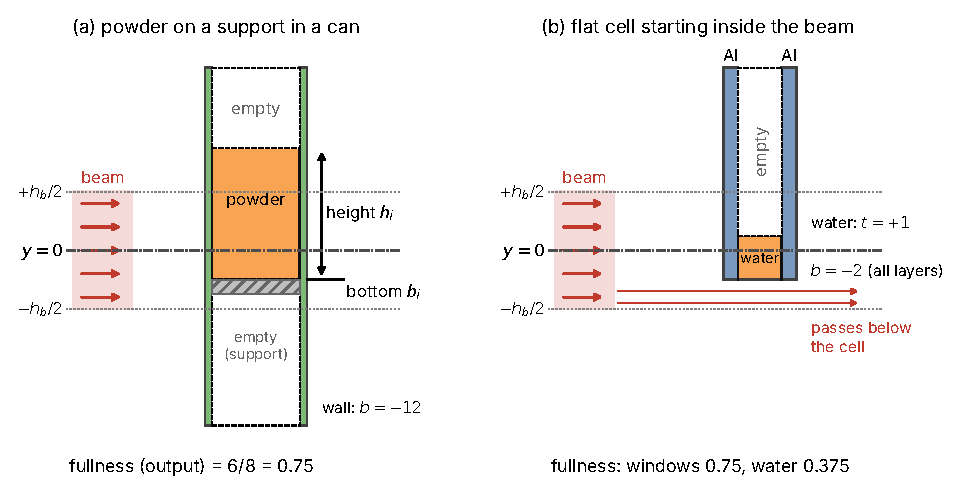
\includegraphics[width=\textwidth]{fig_band_geometry}
  \caption{Layers with their own band (version 2.2), side view. (a)~A powder resting on a support inside a can whose
  bottom is below the beam: the powder goes from $b=-2$ to $t=7$~mm, the wall from $-12$~mm upwards. (b)~A flat cell
  whose windows start inside the beam, at $y=-2$~mm: the lowest 2~mm of the beam pass below the cell. Above the material
  the layers are empty.}
  \label{fig:bandgeom}
\end{figure}

\section{Describing a layer: bottom and height}

The recommended description has two optional fields of \code{Layer}:
\begin{center}\small
\begin{tabular}{@{}lp{11.2cm}@{}}
  \toprule \textbf{Field} & \textbf{Meaning} \\ \midrule
  \code{bottom} & $b_i$: height $y$ of the bottom of the material, in mm from the centre of the beam. \code{None}: the bottom of the sample. \\
  \code{height} & $h_i\geq0$: height of the material in mm; the top is $t_i = b_i + h_i$. \code{None}: up to the top of the sample. \\ \bottomrule
\end{tabular}
\end{center}
\begin{lstlisting}
from sample_base import Layer
Layer("powder", 6.0, 0.25, 0.8, bottom=-2.0, height=9.0)   # from y = -2 to y = +7
Layer("V",      0.2, 0.073, 0.5, bottom=-12.0, height=30.0) # the can
{"name": "powder", "thickness": 6.0, "mu": 0.25, "bottom": -2.0, "height": 9.0}  # as a dict
\end{lstlisting}
The material is always limited to the sample: a band that goes beyond the bottom or the top of the sample is cut there.

\paragraph{Why bottom and height?} They are the two numbers that one measures on a real sample (where the powder
starts, and how high it is), they fix the geometry completely, and they describe the material \emph{outside} the
beam too. That material is not illuminated, but it scatters again the particles that leave the beam region, and it
changes the multiple scattering (Section~\ref{sec:partial-results}). Two other descriptions were possible and were
not chosen as the primary one:
\begin{itemize}
  \item \emph{bottom and top}: equivalent to bottom and height; the height is usually the number one knows (the
        amount of powder), and it cannot be negative by mistake.
  \item \emph{fullness}: one number cannot fix the band once the bottom is free ($f = 0.5$ may be the lower half of
        the beam, the upper half or a band in the middle), and it says nothing about the material outside the beam.
        The fullness is therefore an \textbf{output} of the sample: \code{sample.beam_fullness()}.
\end{itemize}

\section{The height of the sample}

The sample occupies $y_\mathrm{bottom}\leq y\leq y_\mathrm{top}$: the box of a slab, or the length of the cylinders.
It is given as before by \code{height} and \code{y_bottom}. With the layers described by their bands, it can also be
left out: with \code{height=None} the sample is the smallest range that contains the bands of all the layers given
with \code{bottom} and \code{height} (the \emph{envelope}), and \code{y_bottom} defaults to the lowest bottom.
\begin{lstlisting}
can = create_cylindrical_sample(None, [
    Layer("powder", 6.0, 0.25, 0.8,  bottom=-2.0,  height=9.0),
    Layer("V",      0.2, 0.073, 0.5, bottom=-12.0, height=30.0)],
    beam_height=8.0)             # sample from y = -12 to +18
\end{lstlisting}
A layer given without a band fills this envelope.

\section{Fullness: the fraction of the beam covered}

For a beam of height $h_b$ centred on $y=0$, the fullness of layer $i$ is the part of the beam height that its
material covers:
\begin{equation}
  f_i = \frac{\max\bigl(0,\ \min(t_i, h_b/2) - \max(b_i, -h_b/2)\bigr)}{h_b}.
  \label{eq:fullness-general}
\end{equation}
It is 1 if the material covers the whole beam, and 0 if the beam passes completely above or below it.
\code{sample.beam_fullness()} returns it for every layer (it needs the beam height, given when the sample is created
or as an argument), and \code{summary()} shows it in parentheses. With a uniform beam, the number of particles that
interact in a layer is proportional to $f_i$, wherever the band is (Example~10 and Figure~\ref{fig:bandpos}). This is
the value of \code{/fullness} in \textsc{correct}; the comparison with \textsc{pycorrect} shows when the correction of
\textsc{correct} based on it is exact.

\section{The forms of version 2.0}
\label{sec:legacy}

The level of the material can still be given relative to the bottom of the sample:
\begin{description}
  \item[Fill height $h$] (\code{fill_height}, or the 5th element of a tuple): material from the bottom of the sample up
        to $y_\mathrm{bottom}+h$. It is the same as \code{bottom=y_bottom, height=h}.
  \item[Fullness $f$] (\code{fullness}): material from the bottom of the sample up to the level $-h_b/2 + f\,h_b$, i.e.\
        covering the lower fraction $f$ of the beam. To turn it into a level the sample needs the beam height:
        create it with \code{beam_height=...}.
\end{description}
\code{bottom}/\code{height} cannot be combined with \code{fill_height}/\code{fullness} in the same layer; the layers of
one sample can use different forms.

\begin{figure}[H]
  \centering
  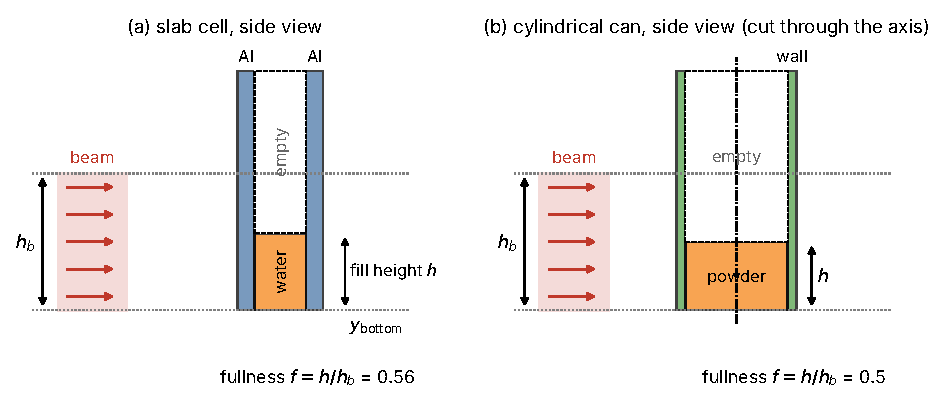
\includegraphics[width=\textwidth]{fig_partial_geometry}
  \caption{The description of version 2.0, side view. (a)~Flat cell: two aluminium windows (full) and water up to a
  fill height $h$. (b)~Cylindrical can: the wall is full and the powder reaches the height $h$. Here the bottom of the
  sample is at the bottom of the beam, so the fullness is simply $f=h/h_b$.}
  \label{fig:partialgeom}
\end{figure}

\begin{warn}[Fullness 1 means completely full]
A layer with \code{fullness=1} is taken as \emph{completely} full, up to the top of the sample, because the fullness
cannot tell how much material lies above the beam. Material above the beam is not illuminated, but it does scatter the
particles that leave the beam region upwards, and this increases the multiple scattering (Section~\ref{sec:partial-results}).
To fill a layer exactly up to the top of the beam, give \code{height} (or \code{fill_height}) instead.
\end{warn}

\section{Creating a sample}

The functions that build the samples accept \code{height=None} and two optional arguments:

\begin{fnbox}{create\_slab\_sample(width, height, layers, z\_front=0, plane\_angle\_deg=90, y\_bottom=None, beam\_height=None)}
\code{height}: height of the slab (mm), or \code{None} for the envelope of the layers.
\code{y_bottom}: height of the bottom of the sample (mm); default centred, or the lowest bottom of the layers.
\code{beam_height}: beam height (mm), needed for \code{fullness} and \code{beam_fullness()}.
\end{fnbox}
\begin{fnbox}{create\_cylindrical\_sample(height, layers, y\_bottom=None, beam\_height=None)}
The same arguments for concentric cylinders.
\end{fnbox}
\begin{fnbox}{make\_sample(geometry, layers, height=None, width=None, plane\_angle\_deg=90, y\_bottom=None, beam\_height=None)}
The factory passes them on to the geometry chosen.
\end{fnbox}

All the ways of writing a layer:
\begin{lstlisting}
from sample_base import Layer

Layer("water", 3.0, 0.56, 1.0, bottom=-2.0, height=3.0)    # 2.2: band from -2 to +1
{"name": "water", "thickness": 3.0, "mu": 0.56, "bottom": -2.0, "height": 3.0}
("water", 3.0, 0.56, 1.0, 4.0)                             # 2.0: fill height (5th element)
Layer("water", 3.0, 0.56, 1.0, fill_height=4.0)            # 2.0
Layer("water", 3.0, 0.56, fullness=0.5)                    # 2.0: lower half of the beam
\end{lstlisting}
Layers computed from their chemical formula (Chapter~\ref{ch:builder}) accept the same arguments:
\begin{lstlisting}
props = compute_layer_properties("D2O", 6.0, "D2O", 1.107, cross_sections={...})
props.as_layer(bottom=-2.0, height=9.0)  # Layer object
props.as_tuple(fill_height=4.0)          # 5-element tuple (version 2.0 form)
build_layer("D2O", 6.0, "D2O", 1.107, cross_sections={...}, bottom=-2.0, height=9.0)
\end{lstlisting}

\section{What the sample tells you}

\begin{center}\small
\begin{tabular}{@{}>{\raggedright\arraybackslash}p{5.2cm}p{9.6cm}@{}}
  \toprule \textbf{Attribute or method} & \textbf{Content} \\ \midrule
  \code{sample.summary()} & the table of layers has a column \code{material y (mm)}: the band of the material, \code{full} or \code{empty}; with the beam height known, the fullness is shown in parentheses \\
  \code{sample.fill_bottoms}, \code{sample.fill_tops} & bottom $b_i$ and top $t_i$ of the material of each layer (mm, lab $y$), limited to the sample \\
  \code{sample.fill_heights} & height of the material of each layer, $t_i-b_i$ (mm) \\
  \code{sample.partial}, \code{sample.empty} & True for the layers with an empty part (below or above the material); True for the layers without material \\
  \code{sample.fill_levels} & all the bottoms and tops that lie inside the sample: the horizontal planes where the material changes \\
  \code{sample.has_partial_layers} & True if at least one layer is partially filled \\
  \code{sample.beam_fullness(h_b)} & fullness of each layer, eq.~(\ref{eq:fullness-general}); without argument it uses the \code{beam_height} of the sample \\
  \code{sample.y_bottom}, \code{sample.y_top} & bottom and top of the sample (mm) \\
  \code{sample.layer_of_points(p)} & returns $-1$ also for points in the empty part of a layer \\
  \code{sample.contains(p)} & True inside the volume of the sample, empty space included \\ \bottomrule
\end{tabular}
\end{center}

\section{Examples}

Example~10 uses the description of version 2.2:

\pyexample{ex10_layer_bands}

The first table shows the powder on its support: from $-2$ to $+7$~mm, i.e.\ 6 of the 8~mm of the beam (fullness 0.75);
no interaction in the powder happens below $y=-2$. The second table moves a band of powder 4~mm high through the beam: the
interactions in the powder follow the fullness, whatever the position of the band. The last table is the cell of
Figure~\ref{fig:bandgeom}b.

Example~8 uses the description of version 2.0:

\pyexample{ex08_partial_fill}

Its first table shows the half-full can: 4~mm of powder, i.e.\ half of the 8~mm beam. The second block shows how the
interactions change with the fullness. The interactions in the powder are proportional to $f$, since the beam is uniform.
Those in the wall \emph{increase} when the can empties: above the powder the beam reaches the downstream wall without
being attenuated by the powder. The last table shows a cell centred on the beam and filled with 6~mm of water: its level
($y=-4$~mm) is exactly at the bottom of the beam, so its fullness is 0 and the beam only crosses the windows.

\section{How it is computed}
\label{sec:partial-algorithm}

The bottom and the top of the material of layer $i$ are two horizontal planes, $y=b_i$ and $y=t_i$. Its material is the part
of the layer between them. Along a straight path $\vec p+s\,\hat d$ this adds one condition to the ones described in Chapter~\ref{ch:physics}:
\begin{description}
  \item[Slab.] The material of layer $i$ is the intersection of three regions: the box of the sample, the slice of the layer
        ($z_i^\mathrm{lo}\le z'\le z_i^\mathrm{hi}$) and the band of the material ($b_i\le y'\le t_i$). Along a straight line each
        region is an interval of $s$, so the material is crossed during a single interval $[s_0^{(i)},s_1^{(i)}]$, the
        intersection of the three. Its length is the path in the material; sorting the intervals by $s_0$ gives the order in which
        the particle meets the materials, and the next interaction is found by accumulating $\mu_i\,(s_1^{(i)}-s_0^{(i)})$ as before.
        The same intervals are used for the incident beam (the particles start upstream of the sample), so entry through a
        side face or over the material is handled automatically.
  \item[Cylinder.] The crossings of all the bottoms and tops (\code{fill_levels}), $s=(b_i-y)/d_y$ and $s=(t_i-y)/d_y$, are added
        to the breakpoints that cut the path into segments. A segment is then in the material of its layer if its midpoint is
        inside the band of that layer; otherwise it is an empty segment, with $\mu=0$.
\end{description}
In all the geometries a particle can fly through the empty part of a layer and enter another layer, or leave through the top
or the bottom of the sample: multiple scattering through the empty space is followed exactly (Figure~\ref{fig:partialtraj}). For full
layers the new calculation gives the same numbers as before, to rounding errors (Chapter~\ref{ch:validation}).

\begin{figure}[H]
  \centering
  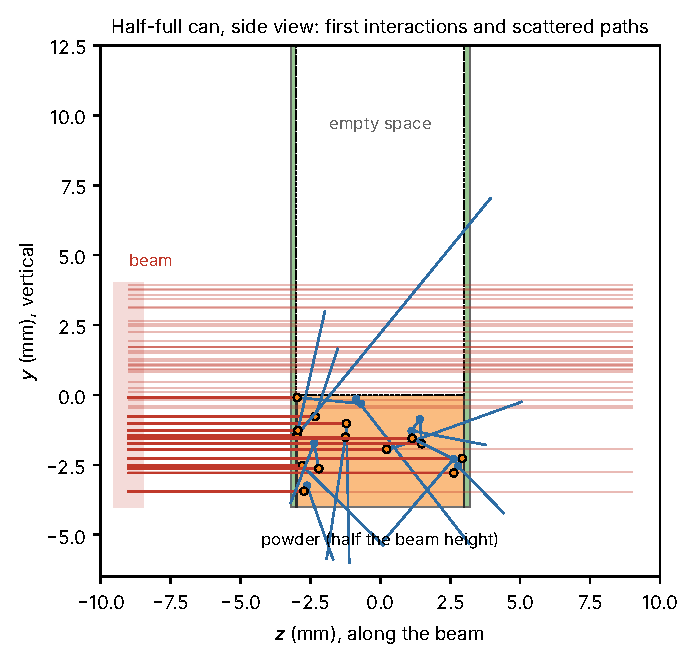
\includegraphics[width=0.78\textwidth]{fig_partial_trajectories}
  \caption{Half-full can in side view (projection on the vertical plane of the beam). Red: incident particles; the faint
  lines are particles that do not interact, most of them above the powder. Dots: first interactions. Blue: the following
  scattering events and the final exit; some particles go up into the empty space, cross it and hit the wall or leave
  through the top.}
  \label{fig:partialtraj}
\end{figure}

\section{Results}
\label{sec:partial-results}

Figure~\ref{fig:partialfull} shows what happens in the example can (powder $\mu=0.25$~mm$^{-1}$, scatter fraction 0.8;
vanadium wall 0.2~mm, $\mu=0.073$~mm$^{-1}$, scatter fraction 0.5; beam $8\times8$~mm, bottom of the can at the bottom of the beam)
as a function of the fullness, with $4\times10^5$ incident particles per point.

\begin{figure}[H]
  \centering
  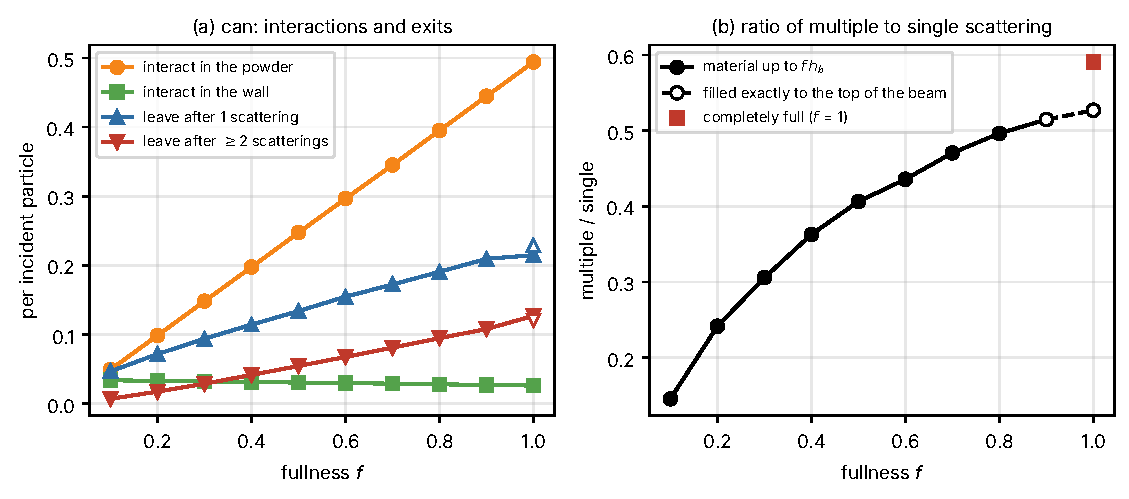
\includegraphics[width=\textwidth]{fig_partial_fullness}
  \caption{Example can versus fullness. (a)~Fraction of the incident particles that interact in the powder and in the wall,
  and that leave the sample after one or after two or more scatterings. Open symbols: can filled exactly up to the top
  of the beam ($h=h_b$). (b)~Ratio of multiple to single scattering.}
  \label{fig:partialfull}
\end{figure}

\begin{itemize}
  \item The scattering in the powder is proportional to the fullness, but the \textbf{multiple scattering grows faster}: the
        ratio of multiple to single scattering goes from 0.15 at $f=0.1$ to 0.52 at $f=0.9$. A thin layer of powder has few
        neighbours to scatter the particles again.
  \item Between ``filled exactly up to the top of the beam'' and ``completely full'' the illuminated material is the same, yet
        the ratio goes from 0.53 to 0.59, and the single scattering leaving the sample decreases (0.229 to 0.215 per incident particle).
        The material \emph{above} the beam scatters again, or absorbs, the particles that go upwards. This is why
        \code{fullness=1} (completely full) and \code{fill_height=beam_height} are different samples.
  \item The wall scatters slightly more when the can empties, because the downstream wall is no longer in the shadow of the
        powder.
\end{itemize}

\paragraph{Position of the material.} Figure~\ref{fig:bandpos} moves a band of powder 4~mm high through the 8~mm beam,
in a can from $-15$ to $+15$~mm. The interactions in the powder, and the single scattering that leaves the sample, follow the
fullness of eq.~(\ref{eq:fullness-general}), as expected. The ratio of multiple to single scattering does not: it is constant
(0.41) while the whole band is inside the beam, and drops to 0.28 when only an edge of the band is illuminated. Particles that
interact near the edge of the material have fewer neighbours to scatter them again. Two samples with the same fullness can
therefore have different multiple scattering.

\begin{figure}[H]
  \centering
  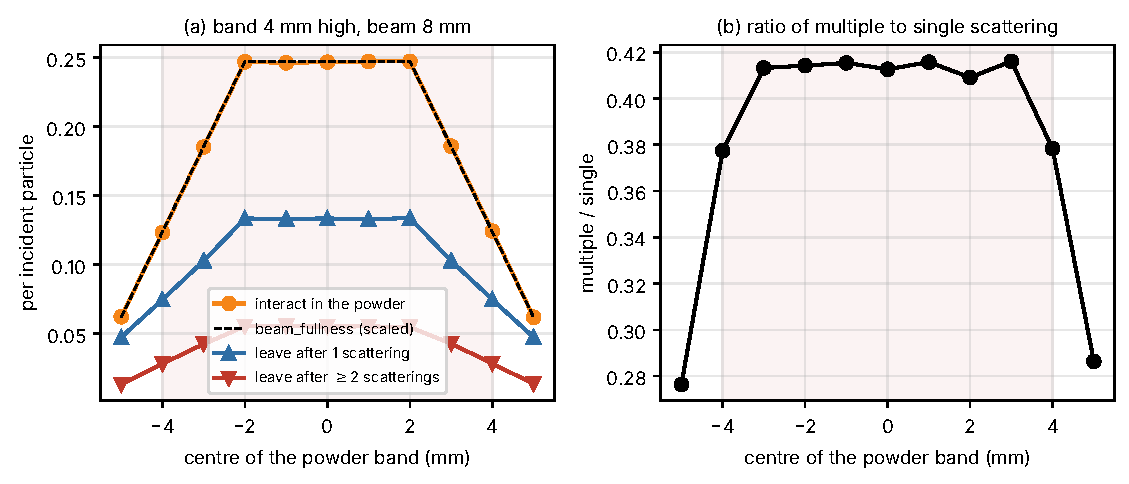
\includegraphics[width=\textwidth]{fig_band_position}
  \caption{A band of powder 4~mm high (example powder, $\mu=0.25$~mm$^{-1}$) moved through an $8\times8$~mm beam (shaded), inside a
  V can from $-15$ to $+15$~mm, $3\times10^5$ particles per point. (a)~Interactions in the powder, the fullness (scaled), and the
  particles that leave after one or more scatterings. (b)~Ratio of multiple to single scattering.}
  \label{fig:bandpos}
\end{figure}

The transmission of the scattered particles (Chapter~\ref{ch:transmission}) changes much less
(Figures~\ref{fig:partialtcyl} and~\ref{fig:partialtslab}). The detector of a two-axis instrument is in the horizontal plane,
so a particle scattered towards it stays at the same height: if it was scattered in the powder, it crosses powder on the way
out whatever the fullness. The transmission increases at low fullness mainly because a larger share of the interactions takes
place in the weakly absorbing wall, above the powder. The partial filling therefore matters mostly through \emph{how much} and
\emph{where} the sample scatters, and through the multiple scattering, rather than through the attenuation of the singly
scattered particles.

\begin{figure}[H]
  \centering
  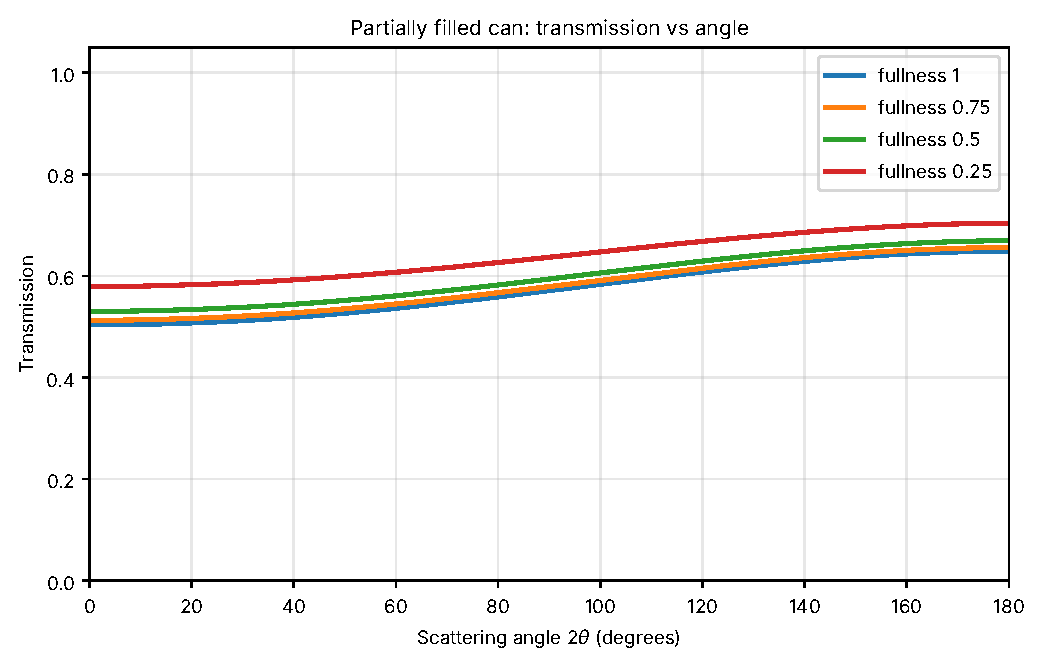
\includegraphics[width=0.78\textwidth]{fig_partial_transmission_cylinder}
  \caption{Example can: transmission versus $\twotheta$ for four values of the fullness.}
  \label{fig:partialtcyl}
\end{figure}

\begin{figure}[H]
  \centering
  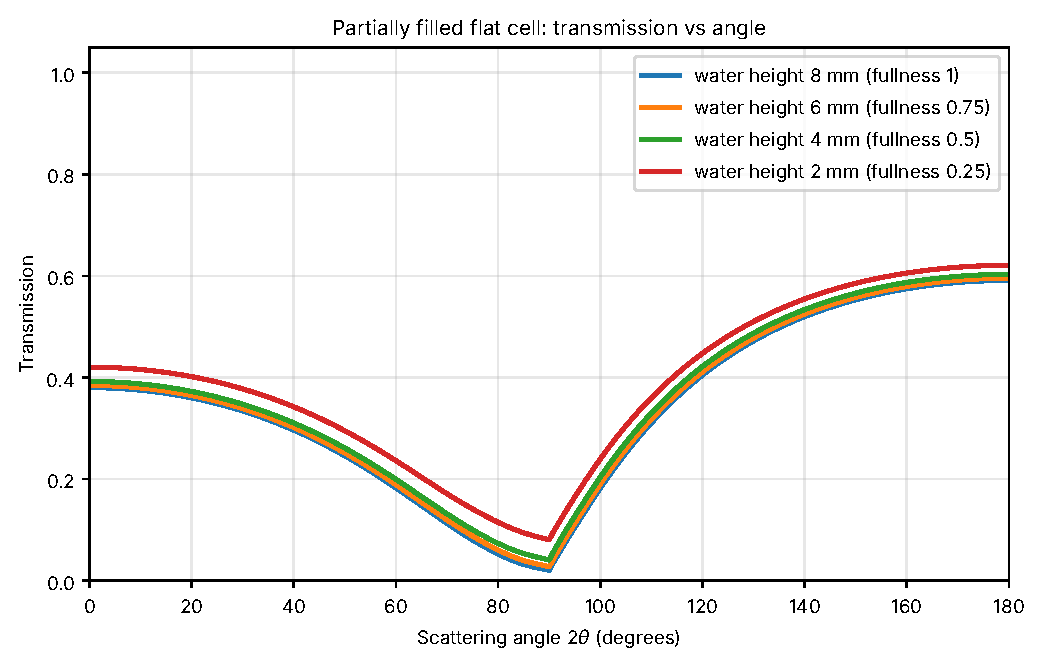
\includegraphics[width=0.78\textwidth]{fig_partial_transmission_slab}
  \caption{Flat cell perpendicular to the beam (aluminium windows of 1~mm, 3~mm of water with $\mu=0.56$~mm$^{-1}$), bottom
  at the bottom of the beam, for four heights of water. The minimum at $90^\circ$ is the direction parallel to the cell.}
  \label{fig:partialtslab}
\end{figure}

\section{With the main script}

\code{run_simulation.py} (Chapter~\ref{ch:main}) has the options \code{--bottom} and \code{--height} (version 2.2), and
\code{--fullness} (version 2.0). They set the band of the layers whose names are listed in \code{CONTENT_LAYERS}, at the top
of the file; the other layers (the walls) stay full. The bottom of the sample is set by \code{SAMPLE_Y_BOTTOM} (default
\code{None}: centred on the beam).
\begin{lstlisting}[style=shell]
python run_simulation.py --geometry cylinder --bottom -6 --height 5
python run_simulation.py --geometry cylinder --fullness 0.5
\end{lstlisting}
\begin{lstlisting}
results = run_simulation("cylinder", bottom=-6, height=5, show=False)
results = run_simulation("cylinder", fullness=0.5, show=False)
\end{lstlisting}
The names of the plot files then end with the band or the fullness, for example\\
\file{transmission\_cylinder\_b-6\_h5.png} or \file{transmission\_cylinder\_full0.5.png}.

\section{Assumptions}

\begin{itemize}
  \item The upper surface of the material is a \textbf{flat horizontal plane}: no meniscus, no slope of a powder. A slab rotated around
        the vertical axis keeps a horizontal surface, as a real cell would.
  \item The space above the material is \textbf{empty} ($\mu=0$). A gas can be added only as a separate full layer.
  \item The surfaces that limit the material are \textbf{horizontal planes} ($y=b_i$ and $y=t_i$). The same holds below the material:
        the band of a powder resting on a support starts at a flat horizontal surface.
  \item The bottom and the lid of a container, and a support, are not layers: the layers of a slab are perpendicular to its normal,
        and those of a cylinder are concentric. A support can be described only by its effect, the empty space below the material.
        A particle reaching the bottom or the top of the sample leaves it.
\end{itemize}

\chapter{Disc samples}
\label{ch:disc}

\section{The idea}

Many flat samples are not rectangular but round: a flat circular cell (window, liquid, window), a pressed pellet, a powder held
between two circular windows, a single-crystal wafer. Version~2.3 adds this geometry: a \textbf{disc} (circular plate) made of
layers stacked along its normal, like a pile of coins of different materials (Figure~\ref{fig:disc}).

\begin{itemize}
  \item Every layer is a disc of the \textbf{same diameter} $D$ (radius $R=D/2$) and of its own thickness.
  \item The centre of the disc is on the \textbf{beam axis}: the disc goes from $y=-R$ to $y=+R$ and from $x=-R$ to $x=+R$.
  \item By default the plane of the disc is \textbf{perpendicular} to the beam. It can be \textbf{rotated} around the vertical axis
        exactly as the slab, with the plane angle $\alpha$ (\code{plane_angle_deg}, Chapter~\ref{ch:geometry}).
  \item A layer has the \textbf{same properties} as in the slab and in the cylinder: label, thickness, $\mu$, scatter fraction and the
        vertical extent of its material (\code{bottom} and \code{height}, Chapter~\ref{ch:partial}). A round cell half filled with a
        liquid is described exactly as a rectangular one.
\end{itemize}
The disc is, in fact, a slab whose section is a circle instead of a rectangle. Everything that does not depend on the shape of the
section (layers along the normal, rotation, frames, partial filling, interaction points, multiple scattering, direct method) is
shared with the slab, and all the analysis modules work with it without any change.

\begin{figure}[H]
  \centering
  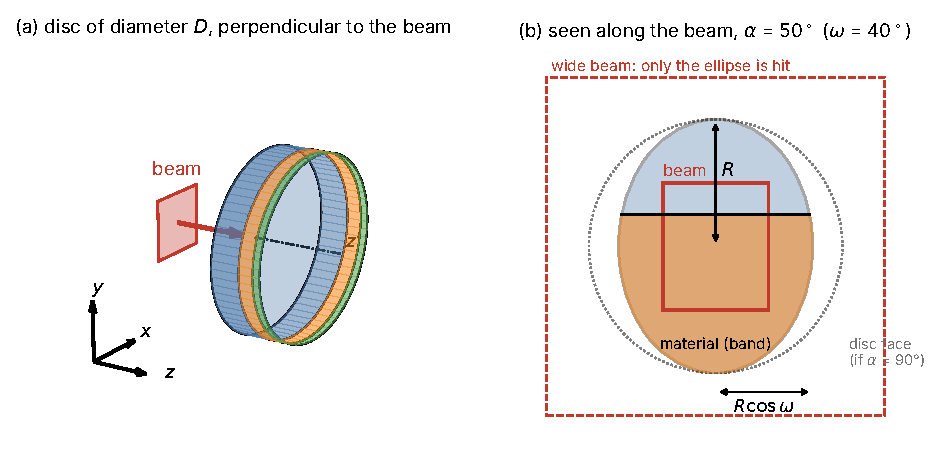
\includegraphics[width=\textwidth]{fig_disc_geometry}
  \caption{Disc geometry. (a)~Three-layer disc perpendicular to the beam; $z'$ is its normal, through the centre of the
  disc and of the beam. (b)~The disc seen along the beam when its plane makes the angle $\alpha=50^\circ$ with the beam: the face
  looks like an ellipse with vertical semi-axis $R$ and horizontal semi-axis $R\cos\omega$, $\omega=90^\circ-\alpha$. A beam
  smaller than the ellipse (solid rectangle) hits the disc everywhere; of a wide beam (dashed) only the part inside the ellipse
  meets the sample. The shaded band is the material of a partially filled layer.}
  \label{fig:disc}
\end{figure}

\section{Geometry and conventions}

The disc uses the sample frame of the slab: $z'$ is the normal of the layers, $x'$ (horizontal) and $y'=y$ (vertical) lie in their
plane, and the front face is at $z'=z_\mathrm{front}$ (default 0). Layer $i$ occupies
\begin{equation}
  x'^2 + y'^2 \le R^2, \qquad z'_i \le z' \le z'_{i+1}, \qquad b_i \le y' \le t_i,
  \label{eq:disc-layer}
\end{equation}
where $z'_i$ are the boundaries of the layers (cumulated thicknesses from the front face) and $b_i$, $t_i$ the bottom and top of
its material (by default the whole disc, $-R$ to $+R$).

\begin{description}
  \item[Rotation.] As for the slab: for $\alpha<90^\circ$ the normal is tilted towards $+x$ by $\omega=90^\circ-\alpha$; for
        $\alpha>90^\circ$ towards $-x$. The axis of rotation is the vertical line through the centre of the front face, which is on the
        beam axis. Seen along the beam the face is an ellipse of semi-axes $R\cos\omega$ (horizontal) and $R$ (vertical).
  \item[Vertical extent.] The sample height is fixed by the disc: $y_\mathrm{bottom}=-R$, $y_\mathrm{top}=+R$. The bands of the layers
        are cut at the rim. In the forms of version~2.0, \code{fill_height} is measured from the lowest point of the disc ($y=-R$) and
        \code{fullness} from the bottom of the beam, as for the other geometries.
  \item[Fullness.] \code{beam_fullness()} is, as always, the fraction of the beam \emph{height} covered by the band of the material
        (eq.~\ref{eq:fullness-general}). For a disc this is also the fraction of the interacting particles only when the beam is
        inside the disc; when the beam is wider than the chord of the disc at some heights, the illuminated width depends on $y$.
\end{description}

\begin{note}[The disc compared with the slab and the cylinder]
For a beam that stays inside the disc and directions that leave through the front or back face, a disc and a slab with the
same layers give \emph{identical} results: the section does not matter. The disc differs from the slab when particles reach its
edge: a beam wider than the disc, scattering nearly parallel to its plane ($\twotheta$ close to $\alpha \pm 90^\circ$, and close to
$90^\circ$ at normal incidence), and multiple scattering, which travels far in the plane. The disc is not a short cylinder: in a
cylinder of \mcams\ the layers are concentric shells around a vertical axis, in a disc they are stacked along a horizontal normal.
\end{note}

\section{Creating a disc sample}

\begin{fnbox}{create\_disc\_sample(diameter, layers, z\_front=0.0, plane\_angle\_deg=90.0, beam\_height=None)}
\code{diameter}: diameter of the disc (mm), the same for all the layers.
\code{layers}: from the front face to the back; tuples, dictionaries or \code{Layer} objects, as for the slab.
\code{z_front}: position of the front face along the normal (mm).
\code{plane_angle_deg}: angle between the beam and the plane of the disc, $0<\alpha<180^\circ$; 90 = perpendicular (default).
\code{beam_height}: height of the beam (mm), needed for \code{fullness} and \code{beam_fullness()}.
Returns a \code{DiscSample}.
\end{fnbox}

\begin{lstlisting}
from disc import create_disc_sample
from sample_base import Layer

cell = create_disc_sample(20.0, [("V",  0.2, 0.046, 0.78),        # front window
                                 ("Ni", 2.0, 0.180, 0.94),        # powder
                                 ("V",  0.2, 0.046, 0.78)])       # back window
tilted = create_disc_sample(20.0, [("V", 0.2, 0.046, 0.78), ("Ni", 2.0, 0.18, 0.94),
                                   ("V", 0.2, 0.046, 0.78)], plane_angle_deg=45)
half = create_disc_sample(20.0, [("V", 0.2, 0.046, 0.78),
                                 Layer("Ni", 2.0, 0.18, 0.94, bottom=-10.0, height=11.0),
                                 ("V", 0.2, 0.046, 0.78)], beam_height=8.0)
\end{lstlisting}
With the factory (Chapter~\ref{ch:sample}) the geometry is \code{"disc"} and the diameter is required; \code{height},
\code{width} and \code{y_bottom} are not used, because the disc is centred on the beam:
\begin{lstlisting}
from sample_factory import make_sample
sample = make_sample("disc", layers, diameter=20.0, plane_angle_deg=60, beam_height=8.0)
\end{lstlisting}
The names \code{"disk"}, \code{"circular"}, \code{"circular plate"} and \code{"round plate"} are accepted as well.

\section{What the disc sample tells you}

A \code{DiscSample} has all the attributes and methods of the slab (Table~\ref{tab:interface} and Chapter~\ref{ch:partial}) and a
few of its own:
\begin{center}\small
\begin{tabular}{@{}>{\raggedright\arraybackslash}p{5.6cm}p{9.2cm}@{}}
  \toprule \textbf{Attribute or method} & \textbf{Content} \\ \midrule
  \code{sample.diameter}, \code{sample.radius} & $D$ and $R$ (mm) \\
  \code{sample.summary()} & table of the layers, with the band of each one and its fullness \\
  \code{sample.face_area_in_beam(w_b, h_b)} & area (mm$^2$) of the part of a uniform $w_b\times h_b$ beam that hits the front face, seen along the beam (ellipse of semi-axes $R\cos\omega$ and $R$); exact for a thin disc. Divided by $w_b h_b$ it is the fraction of the beam that meets the sample. \\
  \code{sample.with_plane_angle(a)} & a copy of the disc with another orientation \\
  \code{sample.boundaries}, \code{z_front}, \code{z_back}, \code{total_thickness} & positions of the layers along the normal (mm), as for the slab \\
  \code{sample.width}, \code{sample.height} & both equal to $D$: the square that contains the disc (used, for instance, to place the start of the particles) \\
  \code{sample.contains(p)} & True for points with $x'^2+y'^2\le R^2$ between the two faces \\ \bottomrule
\end{tabular}
\end{center}
The area of the face seen along the beam is
\begin{equation}
  S = \int_{|y| < \min(R,\,h_b/2)} \min\!\left(2R\cos\omega\,\sqrt{1-y^2/R^2},\; w_b\right) \deriv{y},
\end{equation}
computed by the trapezoidal rule on a fine grid; for a beam larger than the ellipse at normal incidence it is $\pi R^2$.

\section{Example}

\pyexample{ex11_disc}

The beam of $8\times8$~mm is inside the disc, so the fraction of particles that interact in the Ni is the Beer--Lambert value for a
plate, $\e^{-\mu_V t_V}(1-\e^{-\mu_\mathrm{Ni} t_\mathrm{Ni}})$. The transmission is lowest at $90^\circ$, where the scattered particles
travel in the plane of the disc towards its rim. Rotating the disc to $45^\circ$ lengthens the path of the beam in the sample
($1/\sin\alpha$) and more particles interact. With a beam of $30\times30$~mm only the part that hits the face can interact: 35\% of
the beam at normal incidence ($\pi R^2/900$), 25\% at $45^\circ$, where the disc looks narrower. The partially filled disc has Ni up
to $y=+1$~mm, i.e.\ 5 of the 8~mm of the beam (fullness 0.625).

\section{How it is computed}
\label{sec:disc-algorithm}

The slab finds, for every layer, the interval $[s_0^{(i)},s_1^{(i)}]$ of a straight path $\vec p + s\,\hat d$ that lies in its
material, as the intersection of three intervals: the box of the sample, the slice of the layer and the band of the material
(Section~\ref{sec:partial-algorithm}). The disc replaces only the first of them, the \emph{section}: the box is replaced by the
cylinder $x'^2+y'^2\le R^2$ (axis along the normal $z'$) between the front and back faces.

A cylinder is convex, so a straight line is inside it during \emph{one} interval. The line meets its surface when
\begin{equation}
  (p_x + s\,d_x)^2 + (p_y + s\,d_y)^2 = R^2
  \quad\Longleftrightarrow\quad
  a\,s^2 + 2b\,s + c = 0,
\end{equation}
with $a=d_x^2+d_y^2$, $b=p_xd_x+p_yd_y$, $c=p_x^2+p_y^2-R^2$ (sample frame, primes omitted). The two roots
\begin{equation}
  s_\pm = \frac{-b \pm \sqrt{b^2 - a\,c}}{a}
\end{equation}
are where the line enters and leaves the cylinder. If $b^2-ac<0$ the line misses it. If $a=0$ the particle moves along the normal:
it is inside for ever if $c\le0$ and never otherwise. Intersected with the interval between the two faces (the same function as
for the slab), this gives the part of the path inside the disc. From then on the calculation is the slab's: the intervals of
the layers are sorted along the path, their optical depths are accumulated, and the next interaction is found where the
cumulated optical depth reaches the random value $\tau=-\ln(1-u)$ (Chapter~\ref{ch:physics}).

In the code this is a single method. \code{SlabSample} computes the section in \code{_section_interval}, and \code{DiscSample},
a subclass of \code{SlabSample}, redefines it:
\begin{lstlisting}
class DiscSample(SlabSample):
    def _section_interval(self, p, d):
        c_lo, c_hi = _cylinder_interval(p[:, 0], p[:, 1], d[:, 0], d[:, 1], self.radius)
        z_lo, z_hi = _slice_interval(p[:, 2], d[:, 2], self.z_front, self.z_back)
        return np.maximum(c_lo, z_lo), np.minimum(c_hi, z_hi)
\end{lstlisting}
It also redefines \code{contains} (inside the cylinder and between the faces), \code{_clip_inside} (a point that rounding errors
put a few $10^{-15}$~mm outside the rim is moved radially back onto it), \code{summary} and \code{with_plane_angle}, and adds
\code{face_area_in_beam}. Everything else is inherited. The slab itself was only reorganised (the box test moved into
\code{_section_interval}); its results are bit-for-bit those of version~2.2 (Chapter~\ref{ch:validation}).

\section{Results}
\label{sec:disc-results}

The figures of this section use the example layers of the main script (\code{DISC_LAYERS}: Al 2~mm, Fe 1~mm, Cu 0.5~mm, the same as
the example slab), a disc of 20~mm and a beam of $8\times8$~mm.

\begin{figure}[H]
  \centering
  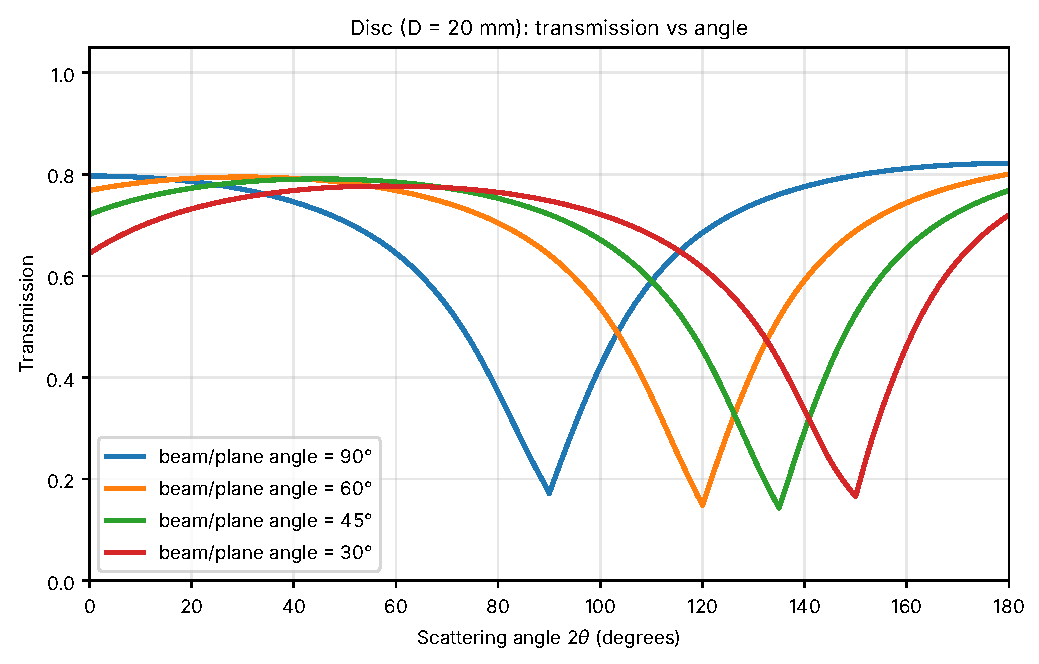
\includegraphics[width=0.78\textwidth]{fig_transmission_disc}
  \caption{Example disc: transmission of the singly scattered particles versus $\twotheta$, for four orientations. The minimum is
  where the scattered particles travel in the plane of the disc, at $\twotheta = 180^\circ-\alpha$ (detector on the side towards which
  the normal is tilted).}
  \label{fig:transdisc}
\end{figure}

\begin{figure}[H]
  \centering
  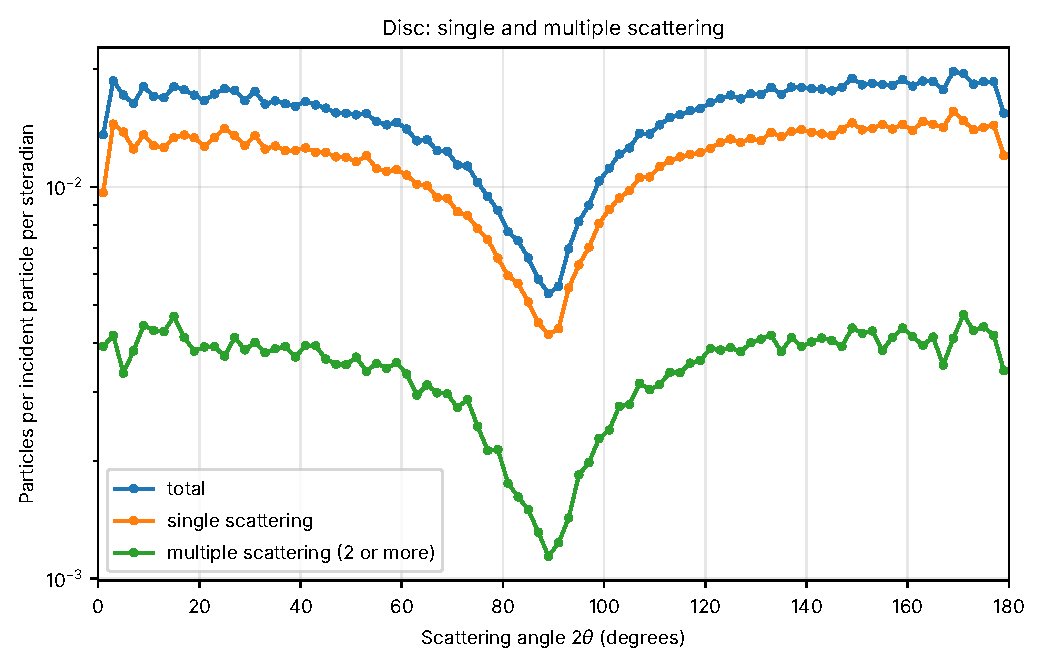
\includegraphics[width=0.78\textwidth]{fig_orders_disc}
  \caption{Example disc perpendicular to the beam: single and multiple scattering per steradian, $10^6$ incident particles.}
  \label{fig:ordersdisc}
\end{figure}

\begin{figure}[H]
  \centering
  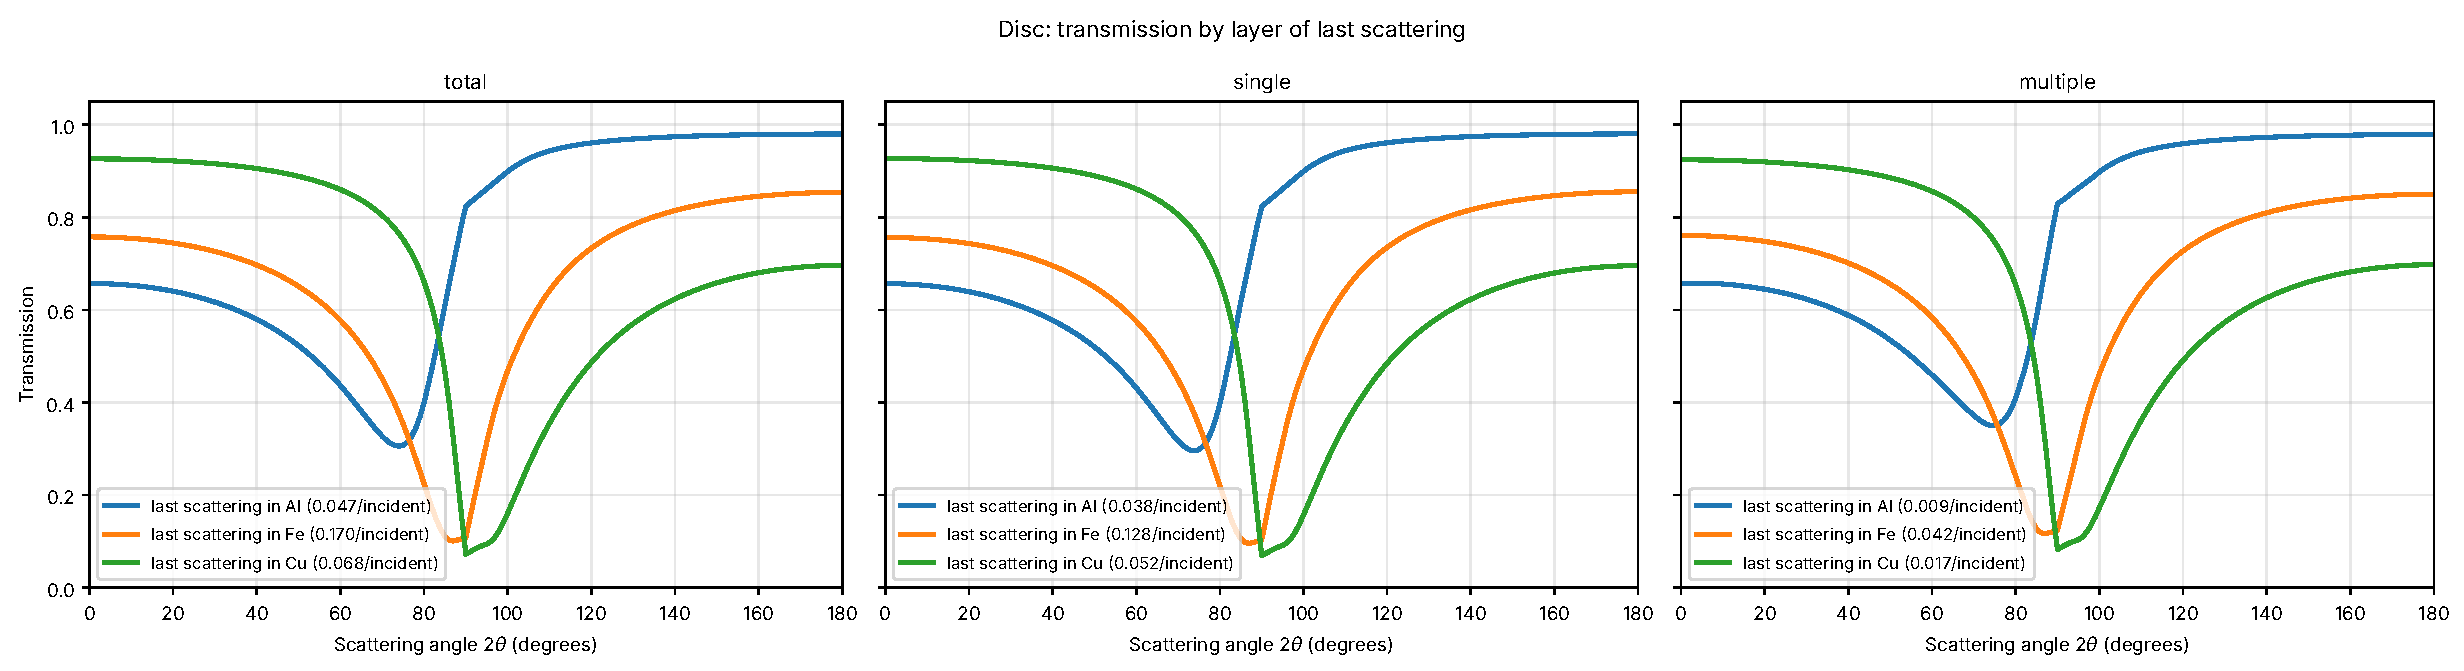
\includegraphics[width=\textwidth]{fig_bylayer_disc}
  \caption{Example disc: transmission by layer of last scattering (Chapter~\ref{ch:lastlayer}).}
  \label{fig:bylayerdisc}
\end{figure}

\paragraph{Disc or square plate?} Figure~\ref{fig:discvsslab} compares the disc with the square slab of side $D$ (the smallest
square that contains it), with the same layers and the same beam.
\begin{itemize}
  \item The transmission is the same at all angles except near $90^\circ$, where the particles leave through the edge. There the
        disc transmits more: at height $y$ its edge is at $\sqrt{R^2-y^2}$ from the axis, closer than the side of the square.
        At $90^\circ$ the transmission is 0.172 (disc) against 0.166 (square) for $D=20$~mm, and 0.430 against 0.382 for
        $D=10$~mm.
  \item The ratio of multiple to single scattering is slightly smaller in the disc, which has less material away from the beam:
        0.214 against 0.230 for $D=9$~mm, 0.299 against 0.303 for $D=20$~mm. The difference vanishes for large discs (0.318 for
        both at $D=40$~mm), where few particles reach the edge.
\end{itemize}

\begin{figure}[H]
  \centering
  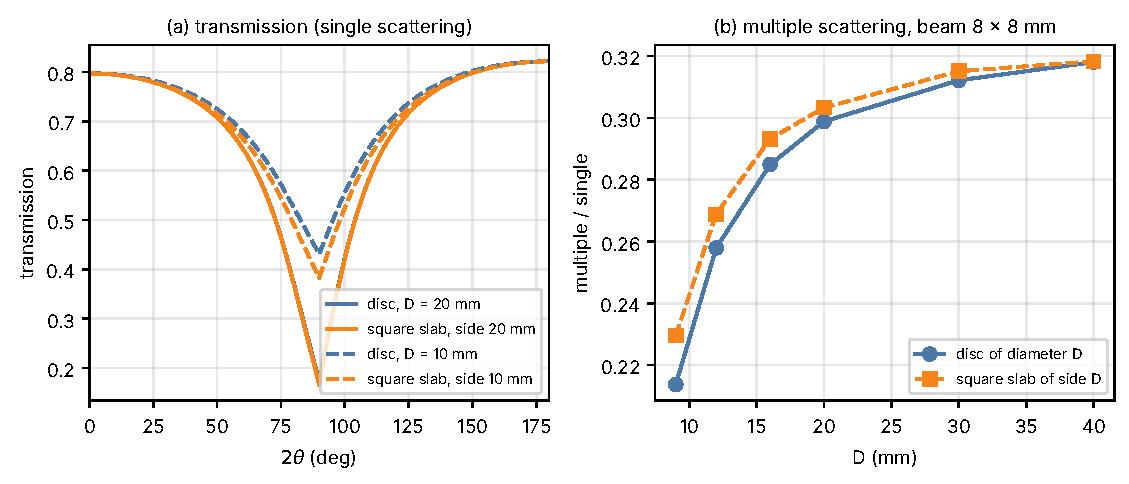
\includegraphics[width=\textwidth]{fig_disc_vs_slab}
  \caption{Disc of diameter $D$ and square slab of side $D$, same layers, normal incidence, beam $8\times8$~mm. (a)~Transmission
  versus $\twotheta$ for $D=20$ and 10~mm. (b)~Ratio of multiple to single scattering versus $D$ ($3\times10^5$ particles per point).}
  \label{fig:discvsslab}
\end{figure}

\paragraph{Validation.} Figure~\ref{fig:discvalid} shows the fraction of a square beam that hits a thin, strongly absorbing disc
(every particle that meets it interacts), for several beam sizes and orientations, against the area of the face seen along the
beam: they agree within the statistical error. The other checks are listed in Chapter~\ref{ch:validation}.

\begin{figure}[H]
  \centering
  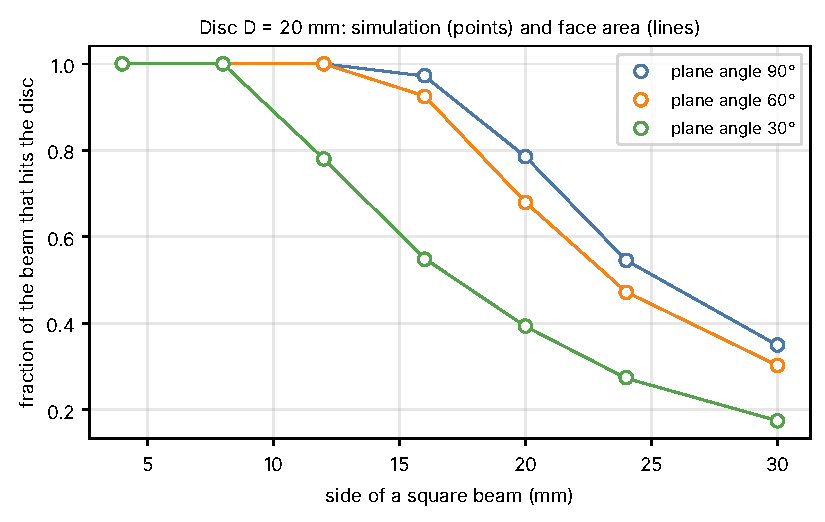
\includegraphics[width=0.78\textwidth]{fig_disc_validation}
  \caption{Disc of 20~mm, 0.01~mm thick, $\mu = 10^4$~mm$^{-1}$: fraction of the beam that interacts (points, $2\times10^5$
  particles each) and \code{face_area_in_beam}$/(w_b h_b)$ (lines), for a square beam of increasing size and three orientations.}
  \label{fig:discvalid}
\end{figure}

\section{With the other modules and the main script}

\begin{itemize}
  \item \code{transmission_vs_angle}, \code{simulate_scattering_orders}, \code{transmission_by_last_layer} and the direct method
        (\code{attenuation_factors_direct}, Chapter~\ref{ch:direct}) accept a disc as they accept a slab or a cylinder.
  \item The main script has the geometry \code{disc}, with the layers \code{DISC_LAYERS} and the diameter \code{DISC_DIAMETER}
        set at the top of \file{run\_simulation.py}; \code{--plane-angle}, \code{--bottom}, \code{--height} and \code{--fullness}
        work as for the slab (Chapter~\ref{ch:main}):
\end{itemize}
\begin{lstlisting}[style=shell]
python run_simulation.py --geometry disc
python run_simulation.py --geometry disc --plane-angle 45
python run_simulation.py --geometry disc --bottom -10 --height 9
\end{lstlisting}

\begin{note}[Discs and \textsc{correct}]
\textsc{correct} (and \textsc{pycorrect}) has no disc geometry: its flat-plate routine \code{PLATE} treats an \emph{infinite} plate.
For a disc larger than the beam this is exact as long as the scattered particles leave through the faces, and it fails near the
grazing directions ($\twotheta\approx 180^\circ-\alpha$ and its mirror), where they leave through the edge. The direct method of
\mcams\ gives the exact factors of the disc at every angle.
\end{note}

\section{Assumptions and limits}

\begin{itemize}
  \item The disc is \textbf{centred on the beam}, horizontally and vertically. An offset disc would need a centre $(x_0, y_0)$ in the
        section test; it is listed among the possible extensions (Chapter~\ref{ch:limits}).
  \item All the layers have the \textbf{same diameter}. A circular cell whose windows are larger than the sample, or a ring that holds
        the sample, needs layers of different diameters (a ring would be a layer with an inner and an outer radius).
  \item The edge of the disc is a plain cylindrical surface: no rim, no clamp, no holder.
\end{itemize}

\chapter{Spherical samples}
\label{ch:sphere}

\section{The idea}

Version~2.4 adds a fourth geometry: \textbf{concentric spheres} (Figure~\ref{fig:sphere}). The sample is a full sphere surrounded by
spherical shells, like an onion: a powder ball in a thin spherical container, a droplet, a single-crystal sphere, a ball of one
material, or a spherical flask partly filled with a liquid.

\begin{itemize}
  \item The common \textbf{centre} of the spheres is the centre of the instrument, on the beam axis ($x=y=z=0$).
  \item The layers are given \textbf{from the inner one outwards}, exactly as for the cylinder: the thickness of the first layer is its
        \textbf{diameter}, and the thickness of every other layer is the \textbf{radial thickness} of its shell,
        \begin{equation}
          r_1 = t_1/2, \qquad r_k = r_{k-1} + t_k \quad (k\ge2).
        \end{equation}
        For instance the thicknesses $(6.0,\,1.0,\,0.5)$~mm give the radii $(3.0,\,4.0,\,4.5)$~mm and an outer diameter of 9~mm.
  \item Every other property of a layer is the same as in the other geometries: label, $\mu$, scatter fraction, and the vertical extent
        of its material (\code{bottom} and \code{height}, Chapter~\ref{ch:partial}).
  \item A sphere looks the same from every direction: there is \textbf{no orientation} parameter, and the sample frame is the lab frame.
\end{itemize}

\begin{figure}[H]
  \centering
  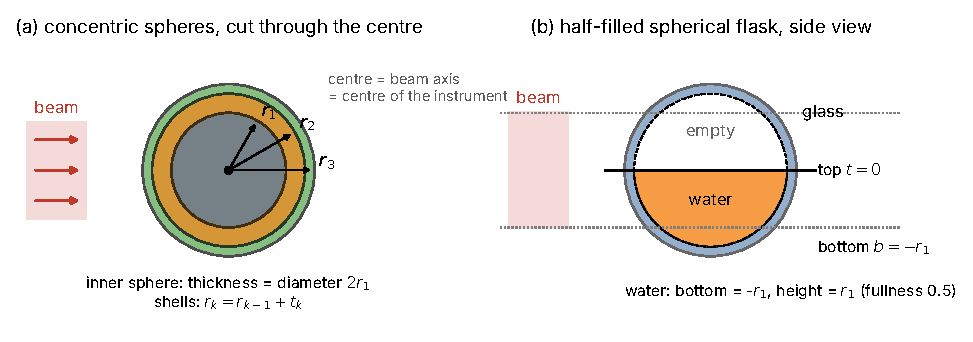
\includegraphics[width=\textwidth]{fig_sphere_geometry}
  \caption{Spherical geometry. (a)~Three concentric spheres cut through their centre, with the radii $r_1<r_2<r_3$; the cut looks the
  same in every plane through the centre. (b)~A spherical flask half filled with water: the glass shell is full, the inner sphere has
  water from its bottom ($y=-r_1$) up to $y=0$, the centre of the beam.}
  \label{fig:sphere}
\end{figure}

\section{Geometry and conventions}

Layer $i$ occupies the shell $r_{i-1} \le |\vec r| \le r_i$ ($r_0=0$), and its material the part of the shell with
$b_i \le y \le t_i$:
\begin{equation}
  r_{i-1} \le \sqrt{x^2+y^2+z^2} \le r_i, \qquad b_i \le y \le t_i .
\end{equation}
\begin{description}
  \item[Vertical extent.] The sample goes from $y=-R_\mathrm{out}$ to $y=+R_\mathrm{out}$ ($y_\mathrm{bottom} = -R_\mathrm{out}$,
        height $2R_\mathrm{out}$). The bands of the layers are cut at the outer sphere. In the forms of version~2.0, \code{fill_height}
        is measured from the lowest point of the sphere, and \code{fullness} from the bottom of the beam.
  \item[Fullness.] \code{beam_fullness()} is the fraction of the beam \emph{height} covered by the band of the material, as for the
        other geometries. For a sphere the illuminated width changes with the height, so it is a fraction of height, not of
        material.
  \item[Detector.] Because of the symmetry, the transmission towards a detector depends only on the angle between the detector and
        the beam, not on the azimuth $\varphi$, as long as the beam illuminates the sphere symmetrically (beam larger than the sphere, or
        square and centred). With a partially filled layer or a rectangular beam smaller than the sphere this symmetry is lost.
\end{description}

\begin{note}[Sphere and cylinder]
In the horizontal plane a sphere and a cylinder of the same radius look alike: both are circles. The difference is vertical. A
particle scattered in a cylinder at height $y$ towards a detector in the horizontal plane crosses a circle of radius $R$; in a sphere it
crosses a circle of radius $\sqrt{R^2-y^2}$, smaller away from the centre. The paths are therefore shorter, the attenuation smaller, and
it changes less with the angle (Section~\ref{sec:sphere-results}).
\end{note}

\section{Creating a spherical sample}

\begin{fnbox}{create\_spherical\_sample(layers, beam\_height=None)}
\code{layers}: from the inner sphere outwards; tuples, dictionaries or \code{Layer} objects, as for the other geometries. The first
thickness is the diameter of the inner sphere, the others radial thicknesses. \code{beam_height}: height of the beam (mm), needed for
\code{fullness} and \code{beam_fullness()}. Returns a \code{SphericalSample}.
\end{fnbox}

\begin{lstlisting}
from sphere import create_spherical_sample
from sample_base import Layer

ball = create_spherical_sample([("Ni", 6.0, 0.180, 0.94),     # inner sphere: diameter 6 mm
                                ("V",  0.2, 0.046, 0.78)])    # container: wall 0.2 mm
flask = create_spherical_sample([Layer("water", 20.0, 0.56, 1.0, bottom=-10.0, height=10.0),
                                 ("glass", 1.0, 0.03, 1.0)], beam_height=8.0)
\end{lstlisting}
With the factory the geometry is \code{"sphere"} (also \code{"spherical"} or \code{"ball"}). Nothing else is needed: the size comes from
the thicknesses, and \code{height}, \code{width}, \code{y_bottom} and \code{plane_angle_deg} are not used.
\begin{lstlisting}
from sample_factory import make_sample
sample = make_sample("sphere", layers, beam_height=8.0)
\end{lstlisting}

\section{What the spherical sample tells you}

\begin{center}\small
\begin{tabular}{@{}>{\raggedright\arraybackslash}p{6.1cm}p{8.7cm}@{}}
  \toprule \textbf{Attribute or method} & \textbf{Content} \\ \midrule
  \code{sample.radii}, \code{sample.inner_radii} & outer and inner radius of each layer (mm) \\
  \code{sample.outer_radius}, \code{sample.diameter} & $R_\mathrm{out}$ and $2R_\mathrm{out}$ (mm) \\
  \code{sample.summary()} & table of the layers: radii, thickness, $\mu$, scatter fraction, band of the material and fullness \\
  \code{sample.section_area_in_beam(w_b, h_b)} & area (mm$^2$) of the part of a uniform $w_b\times h_b$ beam that meets the sphere (the circle of radius $R_\mathrm{out}$ inside the beam rectangle). Divided by $w_b h_b$ it is the fraction of the beam that meets the sample; $\pi R_\mathrm{out}^2$ for a beam larger than the sphere. \\
  \code{sample.y_bottom}, \code{sample.y_top} & $-R_\mathrm{out}$ and $+R_\mathrm{out}$ \\
  \code{sample.contains(p)} & True for the points with $|\vec r|\le R_\mathrm{out}$ \\
  \code{sample.layer_of_points(p)} & layer from the distance to the centre; $-1$ outside, or in the empty part of a layer \\ \bottomrule
\end{tabular}
\end{center}
The section area is
\begin{equation}
  S = \int_{|y| < \min(R_\mathrm{out},\,h_b/2)} \min\!\left(2\sqrt{R_\mathrm{out}^2-y^2},\; w_b\right) \deriv{y},
\end{equation}
computed by the trapezoidal rule on a fine grid.

\section{Example}

\pyexample{ex12_sphere}

The beam ($8\times8$~mm) is larger than the sphere (6.4~mm): only half of it meets the sample ($\pi\,3.2^2/64 = 0.503$). The
transmission is lowest at $0^\circ$ and highest at $180^\circ$, as for a cylinder, but it changes less with the angle. Towards a detector in
the vertical plane ($\varphi=90^\circ$) the transmission is the same as in the horizontal plane, within the statistics: the sphere has no
preferred direction and the square beam illuminates it symmetrically. The flask has water from $y=-10$ to $0$~mm, i.e.\ the lower half
of the 8~mm beam (fullness 0.5).

\section{How it is computed}
\label{sec:sphere-algorithm}

The cylinder cuts every straight path $\vec p + s\,\hat d$ into \emph{segments}, at every place where the material may change: where it
crosses the boundary of a layer, and where it crosses one of the horizontal planes that limit the material of the partially filled
layers. Inside one segment the material is always the same; the layer is found from the distance of the midpoint of the segment to the
axis, and whether it is material or empty space from the height of the midpoint. The path in each layer and the next interaction
follow by walking along the segments (Chapter~\ref{ch:physics}).

The sphere uses exactly the same procedure with three changes:
\begin{enumerate}
  \item \textbf{Crossings of a layer boundary.} A point of the path is on the sphere of radius $r_i$ when $|\vec p + s\,\hat d|^2 = r_i^2$,
        \begin{equation}
          a\,s^2 + 2b\,s + c = 0, \qquad a = \hat d\cdot\hat d = 1,\quad b = \vec p\cdot\hat d,\quad c = |\vec p|^2 - r_i^2,
        \end{equation}
        with the two solutions $s_\pm = (-b \pm \sqrt{b^2 - ac})/a$, where the path enters and leaves the sphere. If $b^2-ac\le0$ it misses
        it. Unlike the cylinder there is no special direction (for the cylinder, a vertical path never crosses the side surface).
  \item \textbf{The layer of a point} is given by its distance to the \emph{centre}, $\sqrt{x^2+y^2+z^2}$, instead of its distance to
        the vertical axis.
  \item \textbf{The outline} of the sample is the outer sphere: there are no flat ends.
\end{enumerate}
In the code, \code{CylindricalSample} computes these three things in three small methods, \code{_shell_interval}, \code{_radius_of} and
\code{_outline_interval}, and \code{SphericalSample}, a subclass of \code{CylindricalSample}, redefines them:
\begin{lstlisting}
class SphericalSample(CylindricalSample):
    @staticmethod
    def _radius_of(x, y, z):
        return np.sqrt(x * x + y * y + z * z)            # distance to the centre

    def _shell_interval(self, p, d, R):
        a = np.sum(d * d, axis=1)
        b = np.sum(p * d, axis=1)
        c = np.sum(p * p, axis=1) - R * R
        disc = b * b - a * c
        crosses = disc > 0.0
        root = np.sqrt(np.where(crosses, disc, 0.0))
        return (np.where(crosses, (-b - root) / a, np.inf),
                np.where(crosses, (-b + root) / a, -np.inf))

    def _outline_interval(self, p, d):
        return self._shell_interval(p, d, self.outer_radius)
\end{lstlisting}
It also redefines \code{contains}, \code{summary} and the constructor (the vertical extent follows from the outer radius), and adds
\code{section_area_in_beam}. Everything else (interaction points, path lengths, next interaction, multiple scattering, direct method) is
inherited. The cylinder itself was only reorganised: its results are bit-for-bit those of version~2.3 (Chapter~\ref{ch:validation}).

\section{Results}
\label{sec:sphere-results}

The figures of this section use the example layers of the main script (\code{SPHERE_LAYERS}: Fe of diameter 6~mm, Al 1~mm, Cu 0.5~mm,
the same as the example cylinder) and a beam of $8\times8$~mm, which is smaller than the sphere (outer diameter 9~mm).

\begin{figure}[H]
  \centering
  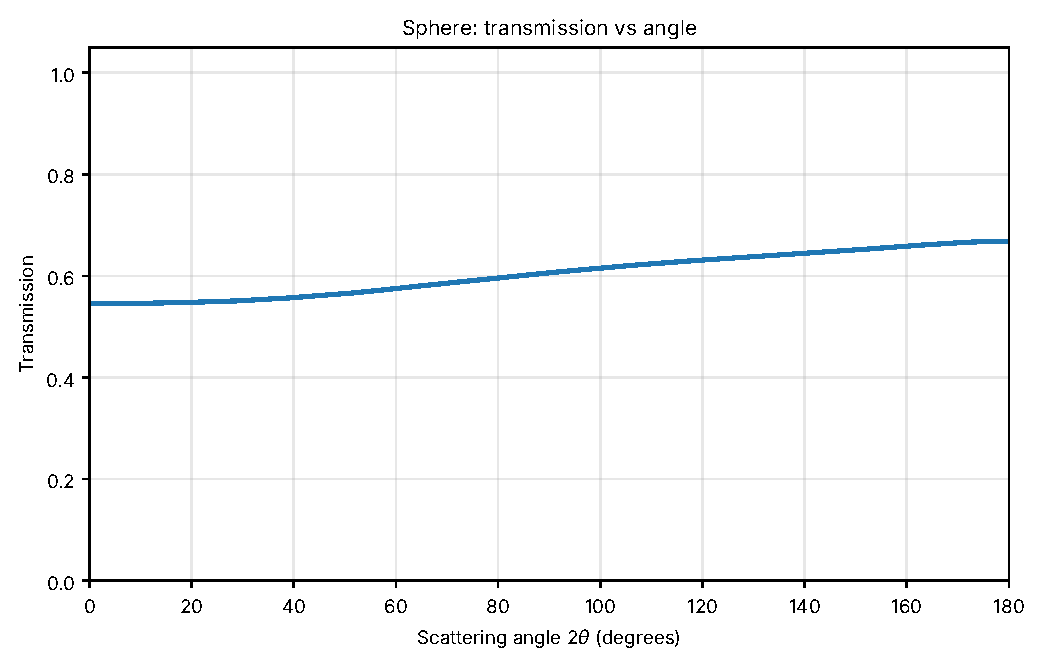
\includegraphics[width=0.78\textwidth]{fig_transmission_sphere}
  \caption{Example sphere: transmission of the singly scattered particles versus $\twotheta$ ($5\times10^4$ particles).}
  \label{fig:transsphere}
\end{figure}

\begin{figure}[H]
  \centering
  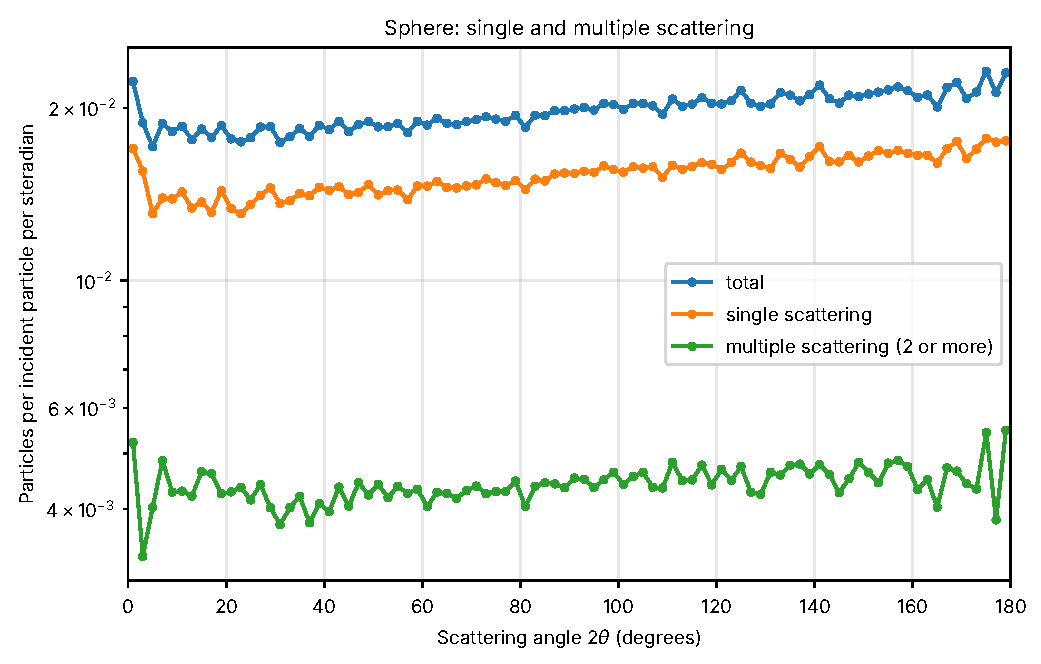
\includegraphics[width=0.78\textwidth]{fig_orders_sphere}
  \caption{Example sphere: single and multiple scattering per steradian, $10^6$ incident particles.}
  \label{fig:orderssphere}
\end{figure}

\begin{figure}[H]
  \centering
  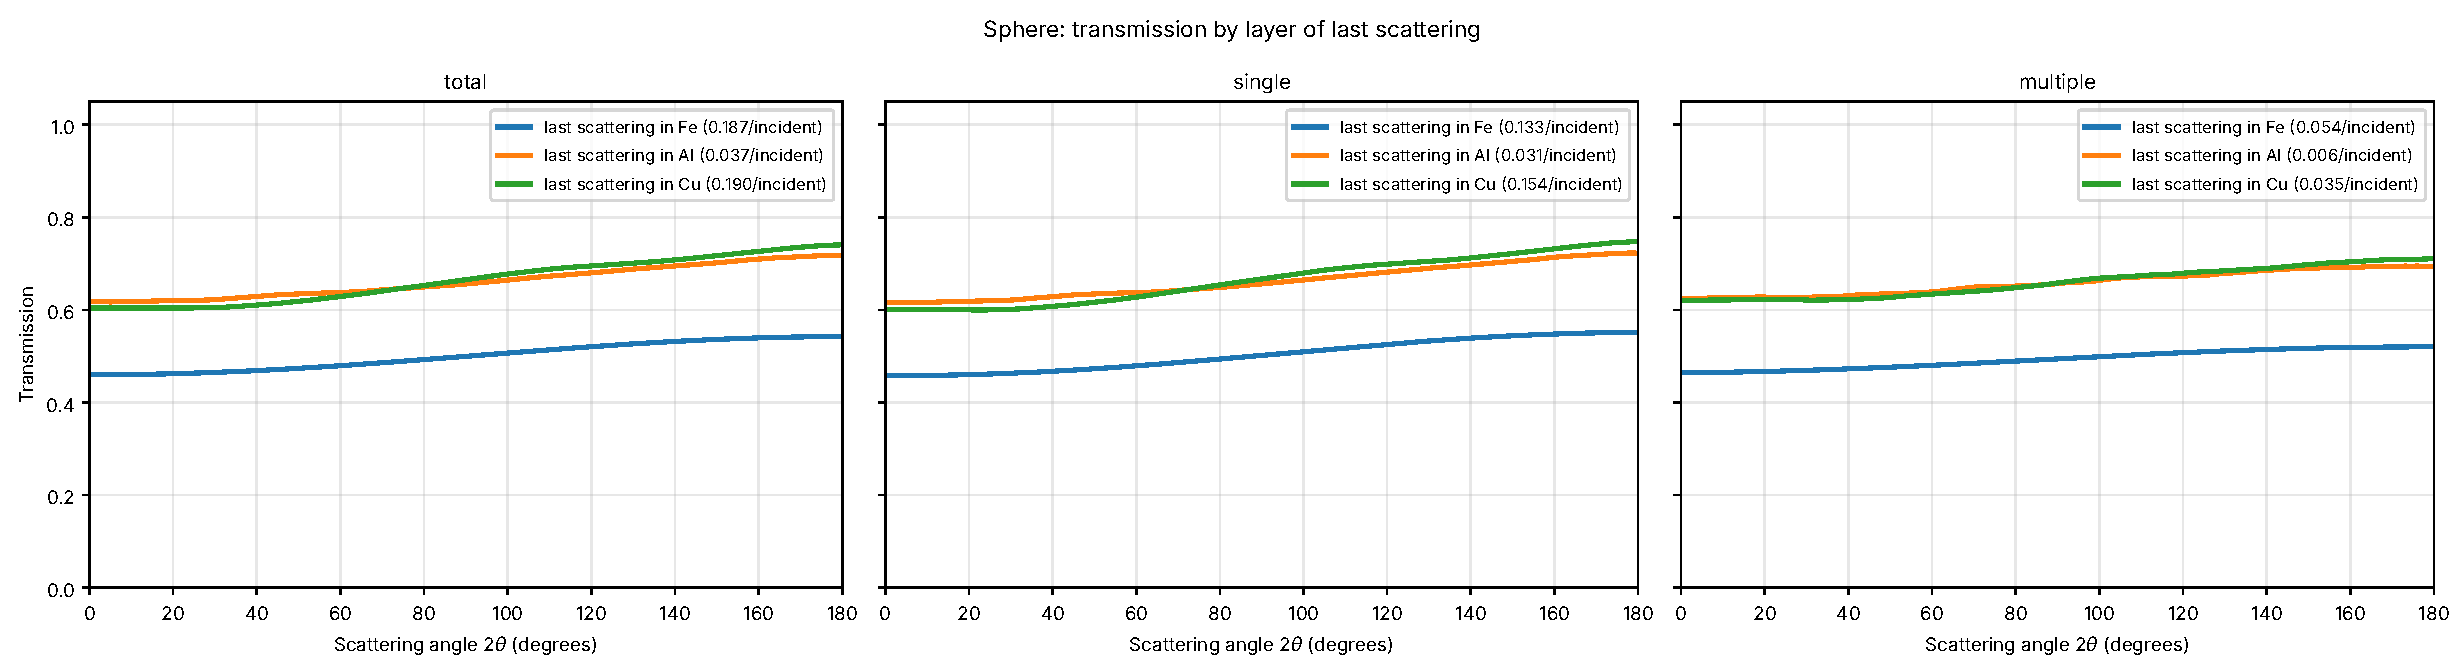
\includegraphics[width=\textwidth]{fig_bylayer_sphere}
  \caption{Example sphere: transmission by layer of last scattering (Chapter~\ref{ch:lastlayer}).}
  \label{fig:bylayersphere}
\end{figure}

\paragraph{Sphere or cylinder?} Figure~\ref{fig:spherevscyl} compares the single-scattering attenuation factor $A(\twotheta)$ (the
Paalman \& Pings factor, computed with the direct method of Chapter~\ref{ch:direct}) of a homogeneous sphere and of a long cylinder
of the same radius (3~mm), for $\mu R=0.5$, 1 and 2, with a beam larger than both.
\begin{itemize}
  \item The sphere attenuates less: $A(0) = 0.483$, 0.242 and 0.071 against 0.434, 0.196 and 0.047 for the cylinder. Its mean chord,
        $4R/3$, is shorter than that of the cylinder, $\pi R/2$.
  \item The attenuation of the sphere changes less with the angle: $A(180^\circ)/A(0)$ is 1.10, 1.37 and 2.52 for the sphere, against
        1.12, 1.50 and 3.31 for the cylinder.
  \item These values can be compared with the tabulated absorption corrections $A^* = 1/A$ for spheres and cylinders
        (\emph{International Tables for Crystallography}, Vol.~C): at $\mu R=1$ and $\twotheta=0$, $A^* = 4.13$ for the sphere and
        $5.10$ for the cylinder here.
\end{itemize}

\begin{figure}[H]
  \centering
  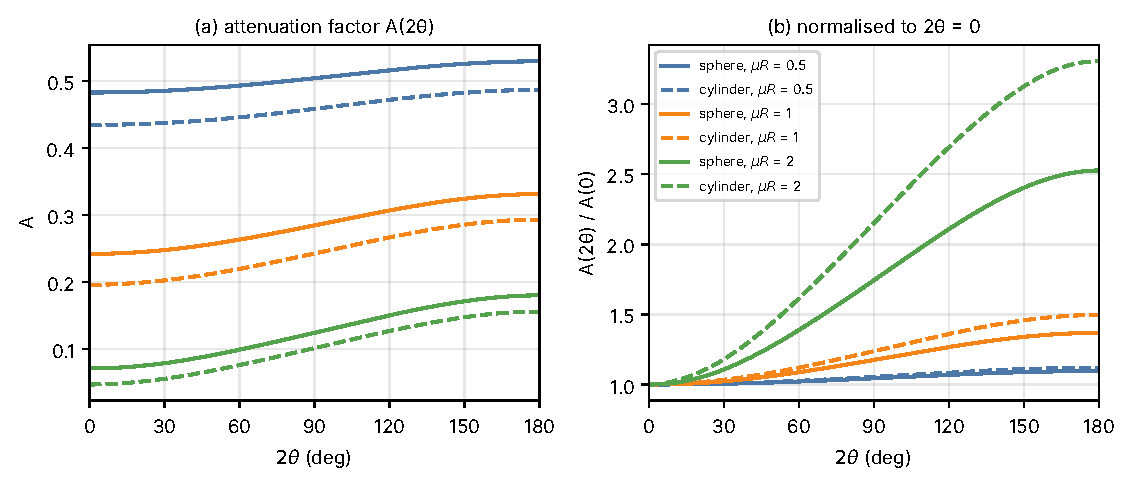
\includegraphics[width=\textwidth]{fig_sphere_vs_cylinder}
  \caption{Attenuation factor of a homogeneous sphere (solid lines) and of a long cylinder (dashed) of radius 3~mm, beam
  $8\times8$~mm, direct method with $6\times10^4$ points, every $1^\circ$. (a)~$A(\twotheta)$. (b)~The same divided by $A(0)$.}
  \label{fig:spherevscyl}
\end{figure}

\paragraph{Validation.} Figure~\ref{fig:spherevalid} compares the fraction of a beam larger than the sphere that interacts in it
with the exact value. A beam line at distance $s$ from the centre crosses a chord $L = 2u$, $u = \sqrt{R^2-s^2}$; with the area element
$2\pi s\,\deriv s = 2\pi u\,\deriv u$,
\begin{equation}
  P_\mathrm{int} = \frac{2\pi}{w_b h_b}\int_0^R \left(1-\e^{-2\mu u}\right) u\,\deriv u .
\end{equation}
The other checks are listed in Chapter~\ref{ch:validation}.

\begin{figure}[H]
  \centering
  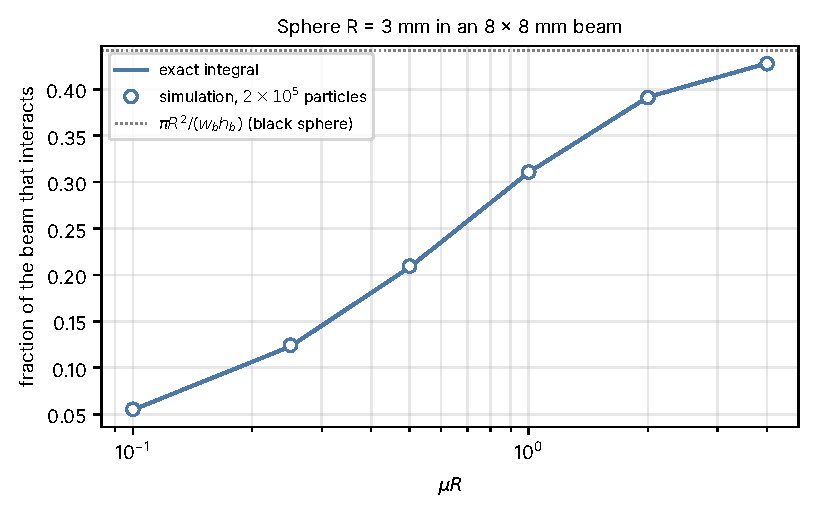
\includegraphics[width=0.75\textwidth]{fig_sphere_validation}
  \caption{Homogeneous sphere of radius 3~mm in an $8\times8$~mm beam: fraction of the beam that interacts, simulation (points) and
  exact integral (line), versus $\mu R$. For large $\mu R$ every particle that meets the sphere interacts: the fraction tends to
  $\pi R^2/(w_bh_b)$ (dotted).}
  \label{fig:spherevalid}
\end{figure}

\section{With the other modules and the main script}

The analysis functions accept a sphere as any other sample:
\begin{itemize}
  \item \code{transmission_vs_angle} (Chapter~\ref{ch:transmission});
  \item \code{simulate_scattering_orders} (Chapter~\ref{ch:scattering});
  \item \code{transmission_by_last_layer} (Chapter~\ref{ch:lastlayer});
  \item \code{attenuation_factors_direct} and the other functions of the direct method (Chapter~\ref{ch:direct}).
\end{itemize} The main script has the geometry \code{sphere}, with the layers \code{SPHERE_LAYERS} set at the
top of \file{run\_simulation.py}; \code{--bottom}, \code{--height} and \code{--fullness} work as for the other geometries
(\code{--plane-angle} is ignored):
\begin{lstlisting}[style=shell]
python run_simulation.py --geometry sphere
python run_simulation.py --geometry sphere --bottom -3 --height 3    # inner sphere half filled
\end{lstlisting}

\begin{note}[Spheres and \textsc{correct}]
\textsc{correct} has no spherical geometry. For a sphere, the attenuation factors (direct method or Monte Carlo) and the multiple
scattering (Monte Carlo) of \mcams{} can replace the cylindrical factors of \textsc{correct} in the same subtraction scheme.
\end{note}

\section{Assumptions and limits}

\begin{itemize}
  \item The spheres are \textbf{concentric} and \textbf{centred on the beam}. An offset sphere would need a centre $(x_0,y_0,z_0)$ in
        \code{_shell_interval} and \code{_radius_of}; it is listed among the possible extensions (Chapter~\ref{ch:limits}).
  \item The material of a partially filled layer is limited by \textbf{horizontal planes}, as in the other geometries (no meniscus).
  \item There is no neck, stem or holder: the sample is only the spheres.
\end{itemize}

\chapter{Physics and algorithms}
\label{ch:physics}

This chapter explains the calculations that all the analysis modules share. Chapter~\ref{ch:geometry} defines the geometry.

\section{Attenuation: the Beer--Lambert law}

A particle that travels a distance $L_i$ in a material with linear attenuation coefficient $\mu_i$ has the probability
$\exp(-\mu_iL_i)$ of crossing it without interacting. After crossing several layers,
\begin{equation}
  T = \exp\!\Big(-\sum_i \mu_i L_i\Big) = \e^{-\tau},\qquad \tau=\sum_i\mu_iL_i,
  \label{eq:beer}
\end{equation}
where $\tau$ is the \emph{optical depth}. This is what \code{sample.transmission(path_lengths)} computes, from a table of
path lengths with one row per particle and one column per layer.

\section{Where does a particle interact?}

The optical depth at which a particle has its first interaction is a random number with the exponential distribution. It is
generated from a uniform random number $u\in[0,1)$ with
\begin{equation}
  \tau = -\ln(1-u).
  \label{eq:tau}
\end{equation}
The particle interacts inside the sample if $\tau$ is smaller than the total optical depth of its path through the sample;
otherwise it crosses the sample without interacting. To convert $\tau$ into a position one follows the particle through the
layers, adding $\mu_iL_i$ until the value $\tau$ is reached; inside that layer the position is found by linear interpolation
(the optical depth grows linearly with distance, with slope $\mu_i$).

\subsection{Slab}

For a slab rotated by $\omega=90^\circ-\alpha$ (Chapter~\ref{ch:geometry}), the beam is oblique with respect to the layers:
the path through a thickness $t$ is $t/\cos\omega$, and the footprint of the beam on the front face is stretched by
$1/\cos\omega$. The optical depth along the beam equals the optical depth along the normal divided by $\cos\omega$, so a random
$\tau$ corresponds to the value $\tau\cos\omega$ measured along the normal. The beam is a ray
\begin{equation}
  x' = x_\mathrm{entry}-\sigma\sin\omega,\qquad z' = z_\mathrm{front}+\sigma\cos\omega,
\end{equation}
as a function of the distance $\sigma$ along it. Because the section of the sample is finite, the function also
takes into account that a particle can \emph{enter through a side face}, and that it can \emph{leave through a side face before
interacting}: such particles are handled correctly (the optical depth only starts to accumulate at the entry point).
In practice the calculation follows each beam particle from a point upstream of the sample and finds, for every layer, the
interval of the path spent in its material; the same intervals serve for partially filled layers (Section~\ref{sec:partial-algorithm}).

\subsection{Disc}

The disc (Chapter~\ref{ch:disc}) is handled exactly as the slab, with one change: the box of the sample is replaced by the
cylinder $x'^2+y'^2\le R^2$ whose axis is the normal $z'$, between the front and back faces. Its intersection with a straight
line is one interval, the solution of a quadratic equation like the one of the next subsection, written in the plane $(x',y')$
of the disc instead of the horizontal plane $(x,z)$ (Section~\ref{sec:disc-algorithm}).

\subsection{Cylinder}

Seen from above, a cylinder of radius $R$ is the circle $x^2+z^2=R^2$. A particle that moves as $\vec p+t\,\hat d$ meets it
where
\begin{equation}
  a\,t^2+2b\,t+c=0,\quad a=d_x^2+d_z^2,\;\; b=x\,d_x+z\,d_z,\;\; c=x^2+z^2-R^2,
\end{equation}
that is, at $t=\big(-b\pm\sqrt{b^2-ac}\big)/a$. Applying this to the radius of every layer, and adding the places where the particle
reaches the top or bottom faces ($y=\pm h/2$), cuts the path into \emph{segments}. Inside a segment the material is always the
same, and it is found from the distance of the segment's midpoint to the axis. The length of the path in each layer is the sum of the
lengths of its segments, and the next interaction is found by accumulating $\mu\,\Delta t$ segment by segment until the random
$\tau$ is reached. Particles parallel to the axis (no horizontal motion) are handled as a special case. When some layers are
partially filled, the crossings of their levels are added to the segments and the segments above the level of their layer get
$\mu=0$ (Section~\ref{sec:partial-algorithm}).

Figure~\ref{fig:traj} (Chapter~\ref{ch:geometry}) illustrates these steps: the incident particles end at their first interaction point, and from there the path towards the detector is followed.

\subsection{Sphere}

The sphere (Chapter~\ref{ch:sphere}) is cut into segments exactly as the cylinder, with spheres instead of cylinders: the path
$\vec p+t\,\hat d$ meets the sphere of radius $r_i$ where $t^2 + 2(\vec p\cdot\hat d)\,t + |\vec p|^2 - r_i^2 = 0$, the layer of a
segment is given by the distance of its midpoint to the centre, and there are no flat ends (Section~\ref{sec:sphere-algorithm}).

\section{Path from a point to the exit of the sample}

Given an interaction point $\vec p$ and a direction $\hat d$ (for instance that of the detector), the function
\code{outgoing_path_lengths} returns the distance travelled in each layer until the particle leaves the sample.
For the \textbf{slab}, the distance to the exit is $t_\mathrm{exit}=\min_k (b_k-p_k)/d_k$, where $b_k$ is the face reached in each coordinate
(the one in the sense of $d_k$); the layer $i$, between the planes $z_i^\mathrm{lo}$ and $z_i^\mathrm{hi}$, is crossed between
$t_a=(z_i^\mathrm{lo}-p_z)/d_z$ and $t_b=(z_i^\mathrm{hi}-p_z)/d_z$, and the path inside it is the overlap of that interval with
$[0,t_\mathrm{exit}]$. For the \textbf{disc} the exit is where the path leaves the cylinder of radius $R$ or one of the faces,
whichever comes first. For the \textbf{cylinder} and the \textbf{sphere} the segments described above are used. Particles travelling parallel to the layers (slab) stay in the layer where they start.

\section{Scattering, absorption and multiple scattering}

At every interaction the particle is scattered with the probability \code{scatter_fraction} of the layer; otherwise it is
absorbed and lost. A scattered particle gets a new direction: the deflection angle $\chi$ relative to the previous direction
is drawn from an angular distribution, and the azimuth around the previous direction is uniform. By default
the distribution is isotropic ($\cos\chi$ uniform in $[-1,1]$). A Henyey--Greenstein distribution \cite{hg} is available,
\begin{equation}
  \cos\chi=\frac{1}{2g}\left[1+g^2-\left(\frac{1-g^2}{1-g+2gu}\right)^{2}\right],
\end{equation}
with $g>0$ forward peaked, $g<0$ backward peaked and $g=0$ isotropic. Any function \code{(n, rng)} $\to$ $n$ values of $\cos\chi$
can be used. After scattering, the particle flies on and either interacts again or leaves the sample
(Chapter~\ref{ch:scattering}).

\section{Example}

\pyexample{ex03_interaction_paths}

The first lines show that 70\,\% of the particles of the beam interact; most of the interactions are in the inner Fe cylinder, which is the most
attenuating one. The paths are averages over the interacting particles: on the way out towards $\twotheta=60^\circ$ they cross
on average 2.2~mm of Fe, 1.2~mm of Al and 0.7~mm of Cu.

\chapter{Transmission versus scattering angle}
\label{ch:transmission}

\section{Definition}

The function \code{transmission_vs_angle} of the module \code{transmission_vs_angle.py} computes, for a list of scattering angles,
the probability that a particle that interacted in the sample leaves it towards the detector without being attenuated:
\begin{equation}
  T(\twotheta)=\Big\langle \exp\!\Big(-\sum_i\mu_iL_i(\twotheta)\Big)\Big\rangle,
\end{equation}
where the average is over all the particles that interacted, and $L_i(\twotheta)$ is the path in layer $i$ from the interaction point to
the exit of the sample, along the direction of the detector. Three remarks:
\begin{itemize}
  \item The attenuation of the incident beam is \emph{not} included again: it is already contained in the interaction points, which are
        drawn with the Beer--Lambert law (Chapter~\ref{ch:physics}).
  \item The same particles are used for every angle, which gives smooth curves.
  \item $T$ does not contain the probability of being scattered towards the detector (a common factor, e.g.\ $1/4\pi$ for
        isotropic scattering).
\end{itemize}

\section{Calling the function}

\begin{lstlisting}
angles, T, f_int = transmission_vs_angle(sample, beam_width, beam_height,
                                         H=None, V=None, n_particles=20000,
                                         angles_deg=None, phi_deg=0.0, rng=None)
\end{lstlisting}
\begin{description}
  \item[\code{sample}] a slab, a disc, a cylinder or a sphere.
  \item[\code{beam_width}, \code{beam_height}] size of the beam (mm); \code{H}, \code{V}: optional profiles.
  \item[\code{n_particles}] number of incident particles.
  \item[\code{angles_deg}] angles $\twotheta$ in degrees; default 0 to 180 in steps of 1.
  \item[\code{phi_deg}] azimuth of the detector (0 = towards $+x$, in the horizontal plane).
\end{description}
It returns the angles, the transmission at each angle, and \code{f_int}, the fraction of the incident particles that interacted (it
includes the particles that miss the sample). Multiplying \code{T} by \code{f_int} gives the fraction of the incident beam that is
scattered \emph{and} leaves the sample towards each angle. The plot is made with
\begin{lstlisting}
plot_transmission(angles, T)                  # one curve
plot_transmission(angles, {"a": T1, "b": T2}) # several curves, with a legend
\end{lstlisting}
(\code{save_as="file.pdf"} saves the figure, \code{show=False} avoids opening the window.)

\pyexample{ex04_transmission}

\section{Results}

\textbf{Slab.} Figure~\ref{fig:tslab} shows the transmission of the example slab for several orientations. At $\alpha=90^\circ$ there is a deep minimum
at $\twotheta=90^\circ$: the scattered particle then travels parallel to the layers and crosses a long path of material. When the slab is
rotated, the minimum moves to $\twotheta=180^\circ-\alpha$, where the direction of the detector is again parallel to the plane of the sample.
The curves also start lower at $\twotheta=0$ when the sample is tilted, because the beam crosses more material.

\begin{figure}[ht]
  \centering
  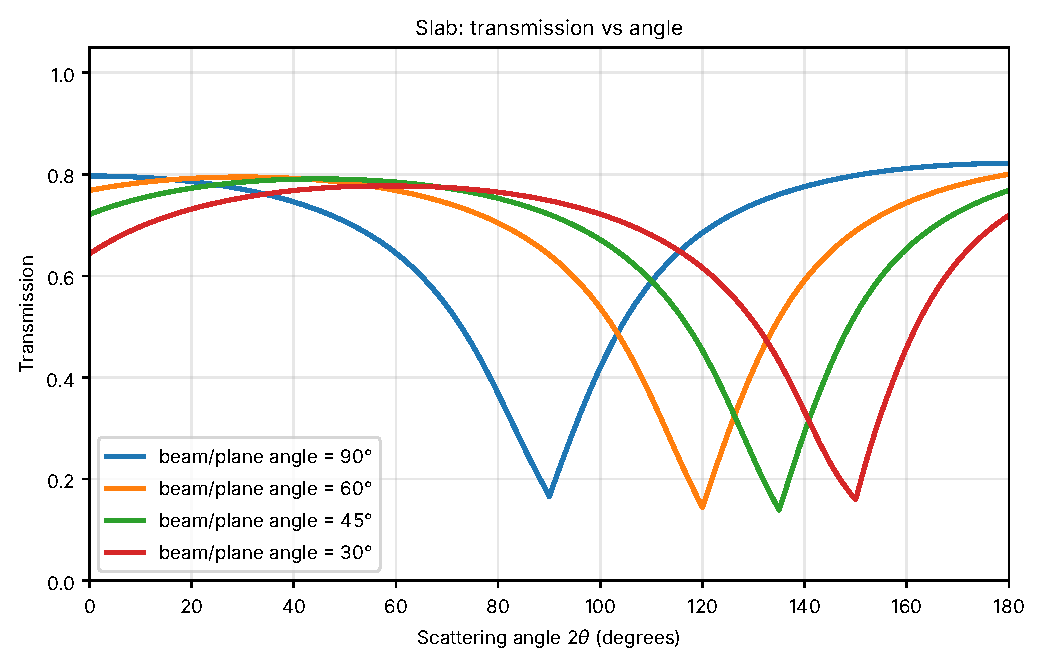
\includegraphics[width=0.8\textwidth]{fig_transmission_slab}
  \caption{Slab: transmission versus $\twotheta$ for four orientations of the sample (angle between the beam and the plane of the
  slab). The minimum follows the direction parallel to the layers.}
  \label{fig:tslab}
\end{figure}

\textbf{Cylinder.} The transmission of the cylinder (Figure~\ref{fig:tcyl}) is smooth and has no minimum: there is no direction along which the path
is especially long. Particles scattered backwards leave through the side from which the beam arrived, crossing less material, so $T$
grows with the angle.

\begin{figure}[ht]
  \centering
  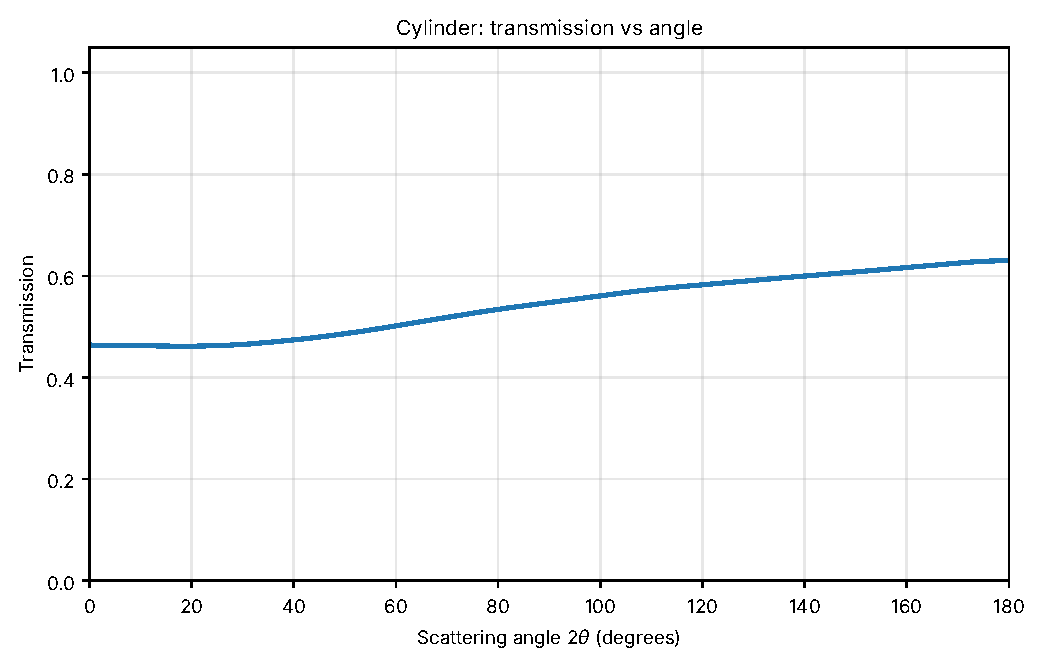
\includegraphics[width=0.8\textwidth]{fig_transmission_cylinder}
  \caption{Cylinder: transmission versus $\twotheta$ (the beam illuminates the whole cylinder, which has a diameter of 9~mm).}
  \label{fig:tcyl}
\end{figure}

\chapter{Single and multiple scattering}
\label{ch:scattering}

\section{What is computed}

The module \code{multiple_scattering.py} follows the particles one by one and \emph{counts} how many leave the sample at each scattering
angle after exactly one scattering (single) or after two or more (multiple). It works with all the geometries.

\section{Algorithm}

\begin{enumerate}
  \item Each particle starts in the beam and flies to its first interaction point in the sample (Chapter~\ref{ch:physics}).
  \item At every interaction it is \textbf{absorbed} (and lost) or \textbf{scattered}, with the probability \code{scatter_fraction} of the layer
        where it is.
  \item A scattered particle gets a new direction, drawn from the angular distribution of one scattering event, and flies on. It either interacts
        again (go to step~2) or leaves the sample.
  \item A particle that leaves the sample is counted in the bin of its final scattering angle $\twotheta$ (the angle between its final direction
        and $+z$), together with its number of scatterings.
\end{enumerate}
Particles that never interact (they miss the sample or cross it) are not scattered and are not counted. The solid angle of a bin of
$\twotheta$ between $a$ and $b$, over an azimuth range $\Delta\varphi$, is $\Delta\Omega=\Delta\varphi(\cos a-\cos b)$; dividing the counts by
the number of incident particles and by $\Delta\Omega$ gives the number of particles per incident particle per steradian, which does not depend
on the width of the bins.

\section{Calling the function}

\begin{lstlisting}
res = simulate_scattering_orders(sample, beam_width, beam_height, H=None, V=None,
                                 n_particles=200000, angle_edges_deg=None,
                                 phi_deg=0.0, phi_halfwidth_deg=None,
                                 deflection_sampler=None, max_orders=200, rng=None)
\end{lstlisting}
\begin{description}
  \item[\code{n_particles}] number of incident particles. Multiple scattering is rare, so use many (\(10^5\)--\(10^6\)).
  \item[\code{angle_edges_deg}] edges of the bins of $\twotheta$ (default: 90 bins of $2^\circ$).
  \item[\code{phi_deg}, \code{phi_halfwidth_deg}] detector window in azimuth: only the particles leaving with an azimuth within
        $\pm$\code{phi_halfwidth_deg} of \code{phi_deg} are counted. The default (\code{None}) counts all azimuths. For a detector in the horizontal plane
        (two-axis instrument) use \code{phi_deg=0} and a small half-width, which needs more particles for the same noise.
  \item[\code{deflection_sampler}] function \code{(n, rng)} returning $n$ values of $\cos\chi$ for one scattering; default isotropic;
        \code{henyey_greenstein(g)} gives a forward ($g>0$) or backward ($g<0$) peaked distribution.
\end{description}
The result \code{res} is a \code{ScatteringResult}:
\begin{center}\small
\begin{tabular}{@{}>{\raggedright\arraybackslash}p{5.6cm}p{9cm}@{}}
  \toprule \textbf{Attribute} & \textbf{Content} \\ \midrule
  \code{res.angles_deg} & bin centres of $\twotheta$ \\
  \code{res.single}, \code{res.multiple}, \code{res.total} & counts per bin of particles scattered once, two or more times, and both \\
  \code{res.counts_by_order} & table with one row for each number of scatterings (1, 2, 3, \ldots) \\
  \code{res.per_steradian(counts)} & converts counts per bin into particles per incident particle per steradian \\
  \code{res.n_incident}, \code{res.n_no_interaction}, \code{res.n_absorbed}, \code{res.n_exited} & bookkeeping: they add up to the incident number \\ \bottomrule
\end{tabular}
\end{center}
The plot is made with \code{plot_scattering_orders(res, per_steradian=True, logy=False)}.

\pyexample{ex05_scattering_orders}

\section{Results}

Figure~\ref{fig:oslab} and Figure~\ref{fig:ocyl} show the three curves for the two example samples (log scale, $10^6$ incident particles).
In the slab, $173{,}576$ of the incident particles are scattered and leave the sample: $133{,}351$ after one scattering and $40{,}225$ after two or more
(23\,\% of the scattered particles). In the cylinder, with a thicker and more attenuating inner part, $192{,}143$ leave after one scattering and
$84{,}180$ after two or more (30\,\%).

\begin{figure}[ht]
  \centering
  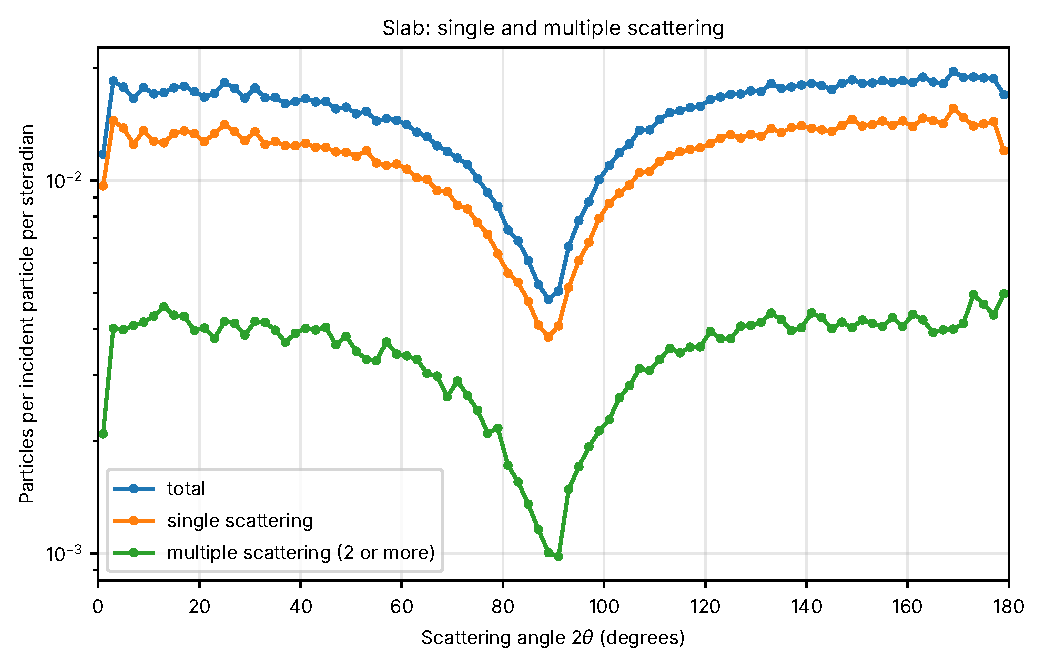
\includegraphics[width=0.8\textwidth]{fig_orders_slab}
  \caption{Slab perpendicular to the beam: total, single and multiple scattering per steradian versus $\twotheta$ ($10^6$ incident
  particles, $2^\circ$ bins). The values near $0^\circ$ and $180^\circ$ are noisy because those bins cover a very small solid angle.}
  \label{fig:oslab}
\end{figure}

\begin{figure}[ht]
  \centering
  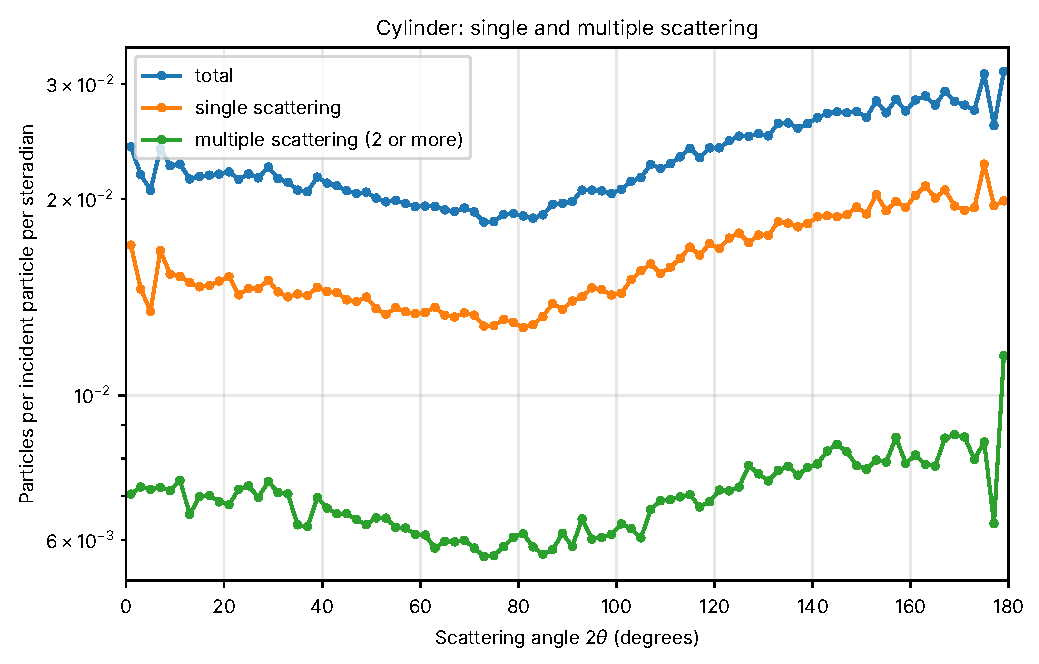
\includegraphics[width=0.8\textwidth]{fig_orders_cylinder}
  \caption{The same for the cylinder. The multiple scattering is a larger part of the total than in the slab.}
  \label{fig:ocyl}
\end{figure}

\section{Statistical error}

The number of counts in a bin follows Poisson statistics: its relative error is $1/\sqrt{N_\mathrm{bin}}$. For example, a bin with 2500 counts has an error of
2\,\%. To reduce the noise, increase \code{n_particles}, use wider bins or accept all azimuths.

\chapter{Transmission by layer of last scattering}
\label{ch:lastlayer}

\section{The question}

A particle that reaches the detector at the angle $\twotheta$ had a last scattering in some layer $k$. From there it crossed several layers on its way out,
each one attenuating it. The function \code{transmission_by_last_layer} (module \code{transmission_by_layer.py}) gives one vector for each layer $k$,
\begin{equation}
  T_k(\twotheta)=\Big\langle \exp\!\Big(-\sum_i\mu_iL_i(\twotheta)\Big)\Big\rangle_{\text{last scattering in layer }k},
\end{equation}
where $L_i$ is the path in layer $i$ from the scattering point to the exit of the sample towards the detector. The sum includes \emph{all} the layers crossed,
not only layer $k$.

\section{How ``last scattering'' is defined}

The particles are followed one by one, as in Chapter~\ref{ch:scattering}. At \emph{every scattering event} the question asked is: ``if this were the last
scattering and the particle went to the detector, how much would it be attenuated?'' This is computed with the exact direction of the detector, for
all the angles at once, which gives smooth curves. Each event is classified by the layer where it takes place and by its order:
\begin{description}
  \item[single] the first scattering of the particle;
  \item[multiple] the second or later scattering;
  \item[total] both together.
\end{description}
The result contains the pure attenuation. The probability of being scattered towards the detector (for instance $1/4\pi$ if the scattering is isotropic)
is a common factor that is not included, as in Chapter~\ref{ch:transmission}; the number of scattering events in each layer is given to weight the layers.

\section{Calling the function}

\begin{lstlisting}
res = transmission_by_last_layer(sample, beam_width, beam_height, H=None, V=None,
                                 n_particles=50000, angles_deg=None, phi_deg=0.0,
                                 deflection_sampler=None, max_orders=200, rng=None)
\end{lstlisting}
\begin{center}\small
\begin{tabular}{@{}>{\raggedright\arraybackslash}p{5.6cm}p{9cm}@{}}
  \toprule \textbf{Result} & \textbf{Content} \\ \midrule
  \code{res.angles_deg} & the angles $\twotheta$ (default 0 to 180, step 1) \\
  \code{res.layer_names} & names of the layers \\
  \code{res.transmission[k]} & vector versus angle: last scattering in layer $k$, all orders \\
  \code{res.transmission_single[k]}, \code{res.transmission_multiple[k]} & the same for first scatterings only, and for second and later ones \\
  \code{res.events(kind)[k]} & number of scattering events in layer $k$; \code{kind} is \code{"single"}, \code{"multiple"} or \code{"total"} \\
  \code{res.events(kind)[k] / res.n_incident} & events in layer $k$ per incident particle (weight of the layer) \\
  \code{res.mean_transmission(kind)} & transmission averaged over all the layers, weighted by the events \\ \bottomrule
\end{tabular}
\end{center}
A layer without scattering events (for example a gap with $\mu=0$) gets NaN. The layers are numbered in the order of the sample (for the cylinder, from the
axis outwards). The plot is made with \code{plot_transmission_by_layer(res, kind="all")}, which draws three panels (total, single, multiple); the
legend gives the events per incident particle in each layer.

\pyexample{ex06_by_layer}

\section{Results}

\begin{figure}[ht]
  \centering
  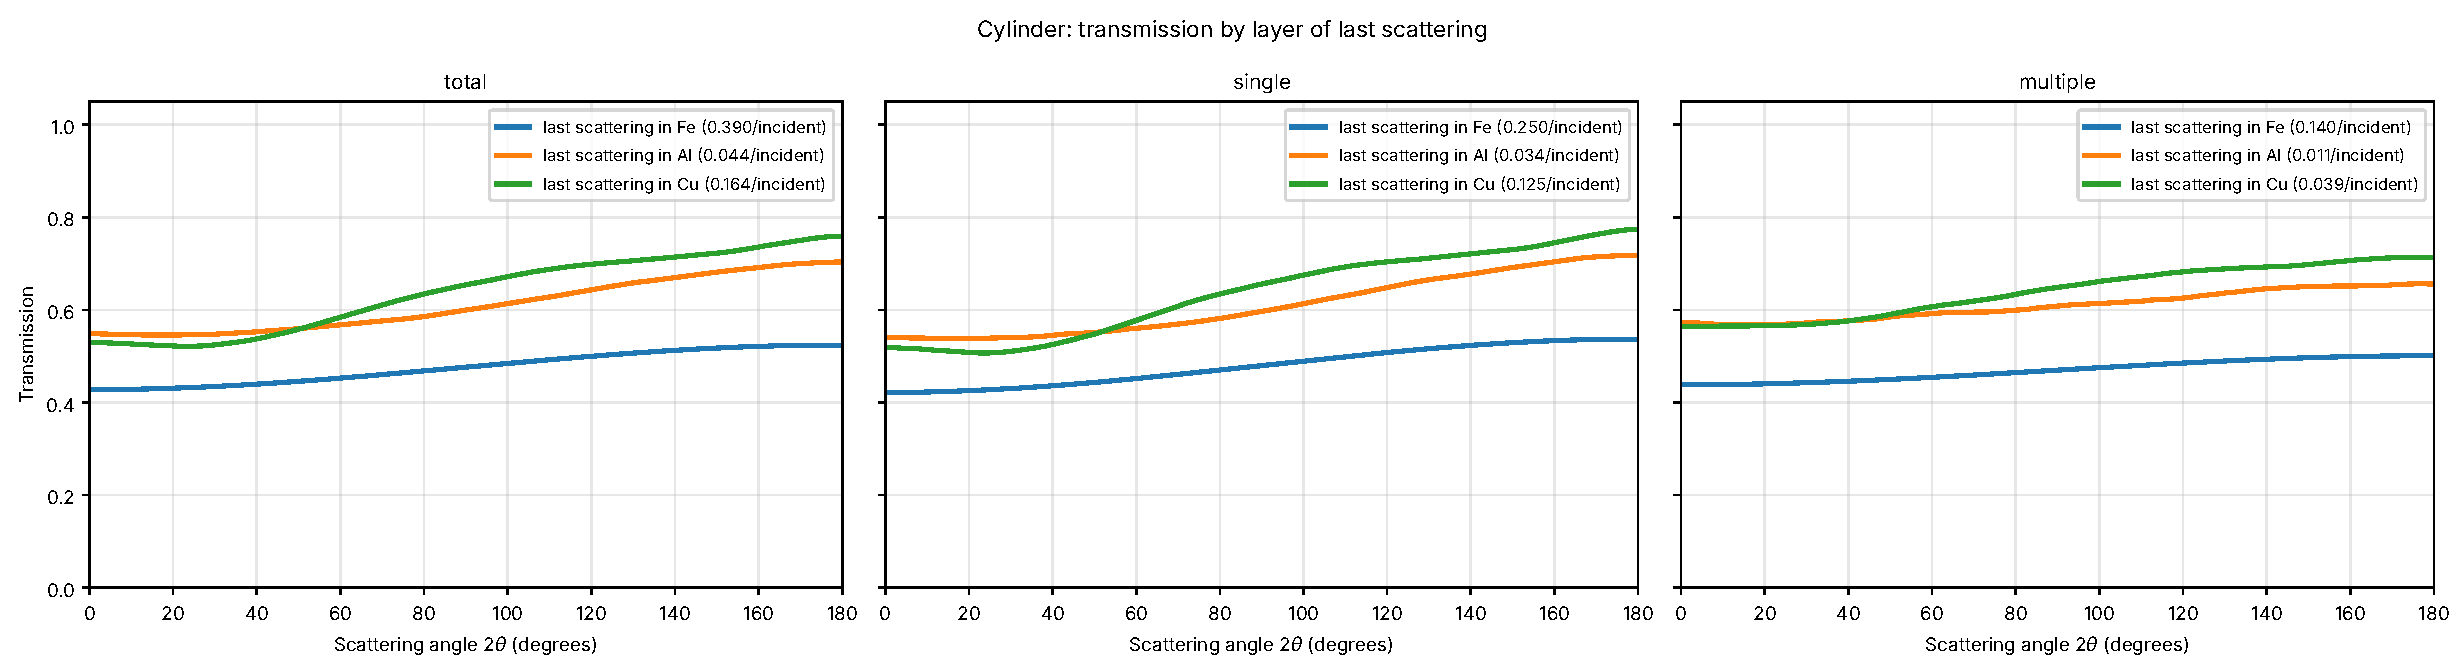
\includegraphics[width=\textwidth]{fig_bylayer_cylinder}
  \caption{Cylinder: transmission versus $\twotheta$ for each layer of last scattering (total, single and multiple scattering). The number in the
  legend is the number of scattering events in that layer per incident particle.}
  \label{fig:blcyl}
\end{figure}

For the cylinder (Figure~\ref{fig:blcyl}), particles whose last scattering was in the inner Fe core have the lowest transmission, since they have to cross the most
material to leave; those scattered in the outer Cu shell are less attenuated, especially towards backward angles. Most of the scattering events take place in the Fe core.

\begin{figure}[ht]
  \centering
  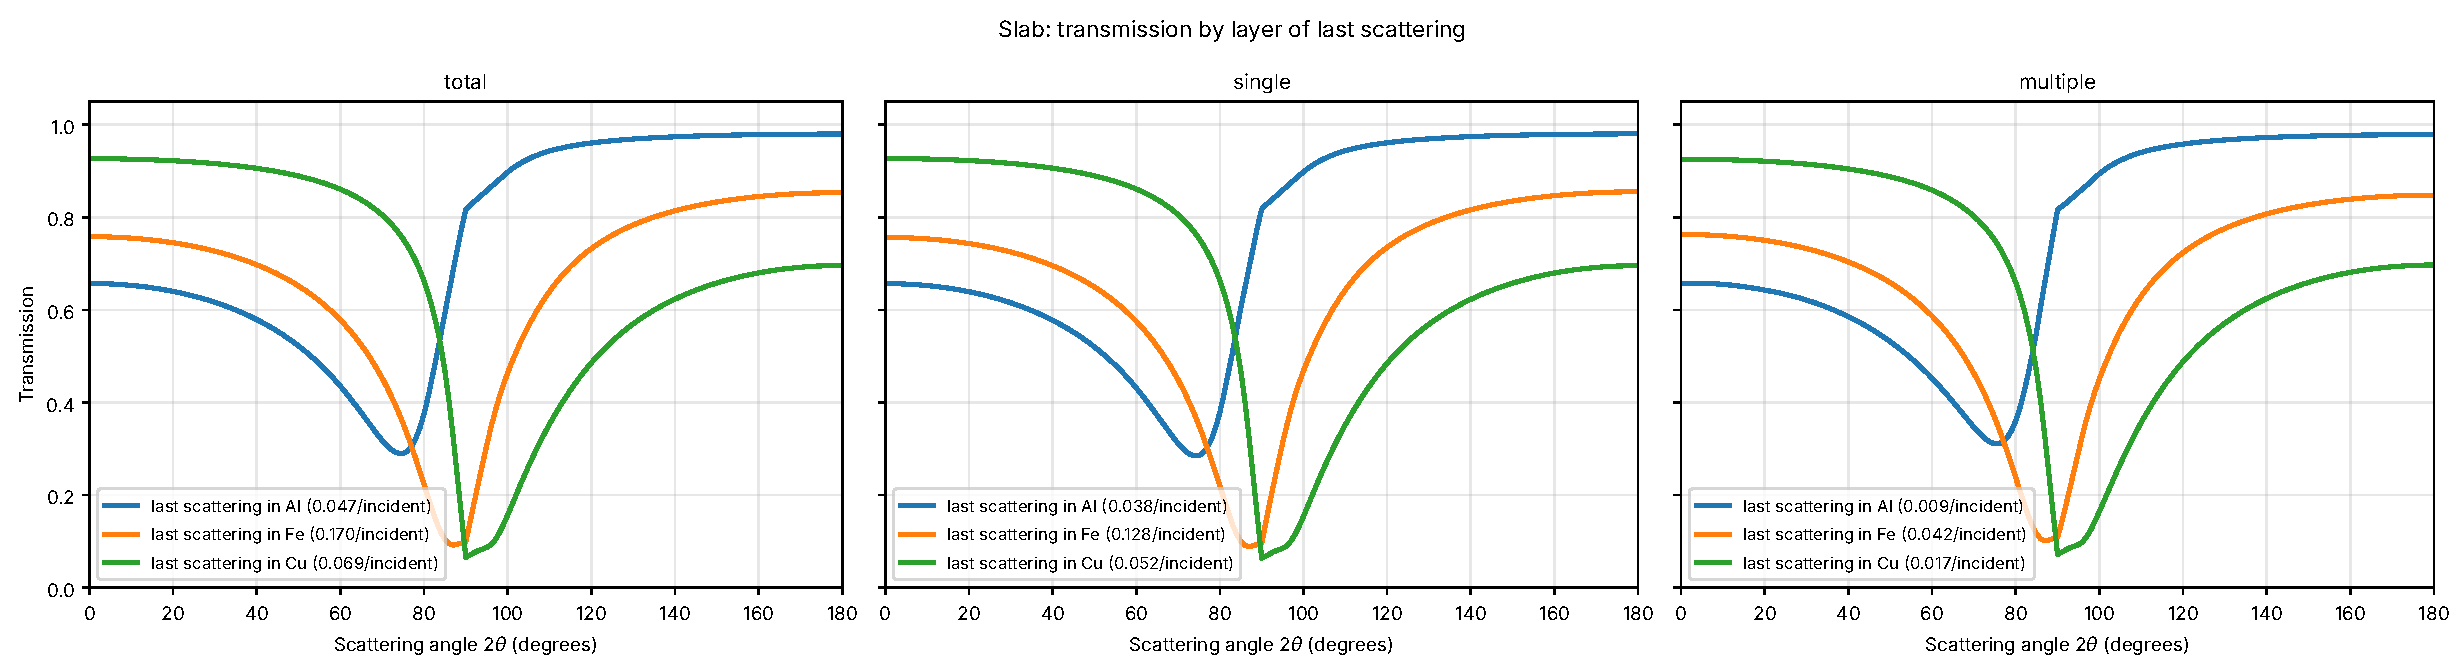
\includegraphics[width=\textwidth]{fig_bylayer_slab}
  \caption{Slab perpendicular to the beam: the same quantity. The steps near $90^\circ$ are real: just below $90^\circ$ a particle scattered in the
  first layer must cross all the others to leave through the back face, whereas just above $90^\circ$ it leaves backwards through the first layer only.}
  \label{fig:blslab}
\end{figure}

\section{Relation with the other functions}

If all the layers have \code{scatter_fraction}\,=\,1, the \emph{single} result averaged over the layers with \code{res.mean_transmission("single")}
is identical (to rounding) to the transmission of Chapter~\ref{ch:transmission}. The \emph{multiple} part is consistent, within the statistical
errors, with the particle-by-particle counts of Chapter~\ref{ch:scattering} (Chapter~\ref{ch:validation}).

\chapter{Direct method: a reference for single scattering}
\label{ch:direct}

\section{Why a second method}

The Monte Carlo of the previous chapters reproduces the attenuation of the incident beam by \emph{where} the particles happen to interact: the
interaction points are drawn with the Beer--Lambert law. This is the natural way to follow particles through many scatterings, but for the
attenuation of \emph{singly} scattered particles it wastes most of the work when a layer attenuates weakly: in a 0.2~mm vanadium wall only about one
incident particle in a hundred interacts, and the other ninety-nine contribute nothing to that layer.

The module \code{direct_attenuation.py} computes the same single-scattering quantities in a different way, the \emph{direct} (or ``expected value'')
method. The attenuation is applied as an exact \emph{weight} instead of a random event, so every sample point contributes. The result is
\begin{itemize}
  \item a precise \textbf{reference} for the Monte Carlo results, to check them and to see their statistical scatter;
  \item the \textbf{Paalman \& Pings attenuation factors} of every layer, for any geometry of \mcams{} (slab or disc at any angle, cylinder, sphere, partially filled
        layers, beam profiles), with error bars;
  \item the exact expected \textbf{single-scattering intensity}, to put on top of the histograms of Chapter~\ref{ch:scattering}.
\end{itemize}
It does \emph{not} replace the Monte Carlo: it contains no multiple scattering, and for strongly attenuating samples the Monte Carlo is the more
efficient of the two (Section~\ref{sec:direct-efficiency}).

\section{The quantity computed}
\label{sec:direct-def}

For a layer $k$ and a scattering angle $\twotheta$, the \textbf{attenuation factor} is the average of the attenuation over the points $\mathbf r$ of the
material of the layer that are lit by the beam:
\begin{equation}
  A_k(\twotheta)=\frac{\displaystyle\int_{V_k} I(x,y)\,\exp\!\Big(-\sum_i\mu_i\big[L^{\mathrm{in}}_i(\mathbf r)+L^{\mathrm{out}}_i(\mathbf r,\twotheta)\big]\Big)\,\deriv V}
                     {\displaystyle\int_{V_k} I(x,y)\,\deriv V},
  \label{eq:Ak}
\end{equation}
where $I(x,y)=H(x)V(y)$ is the beam intensity, $L^{\mathrm{in}}_i$ the path in layer $i$ of the incident beam up to $\mathbf r$, and
$L^{\mathrm{out}}_i$ the path from $\mathbf r$ to the exit of the sample towards the detector. $A_k=1$ without attenuation. For a uniform beam and a
sample taller than the beam this is exactly the factor $A_{s,sc}$, $A_{c,sc}$, \dots{} of Paalman and Pings~\cite{pp}.

The second quantity is the \textbf{mean path} of the beam in the material of layer $k$, averaged over the whole beam (the parts that miss the layer
count as zero):
\begin{equation}
  \langle L_k\rangle=\frac{\int_{V_k} I(x,y)\,\deriv V}{\int_{\text{beam}} I(x,y)\,\deriv x\,\deriv y}.
\end{equation}
$\mu_k\langle L_k\rangle$ is the probability that an incident particle would interact in layer $k$ if there were no attenuation. With the scatter
fraction $f_k$, the singly scattered particles that leave the sample towards $\twotheta$, per incident particle and per steradian, are (isotropic
scattering)
\begin{equation}
  \frac{\deriv N_1}{N\,\deriv\Omega}(\twotheta)=\sum_k\frac{f_k\,\mu_k\,\langle L_k\rangle\,A_k(\twotheta)}{4\pi}.
  \label{eq:single-sr}
\end{equation}

\paragraph{Relation with the Monte Carlo.} \code{transmission_by_last_layer} (Chapter~\ref{ch:lastlayer}) adds up, for the first scatterings in
layer $k$, the outgoing attenuations. Because the interaction points already contain the incident attenuation, the expected value of that sum per
incident particle is $f_k\mu_k\langle L_k\rangle A_k(\twotheta)$. So the Monte Carlo gives the same $A_k$ after dividing by
$f_k\mu_k\langle L_k\rangle$; this is what \code{attenuation_factors_mc} does.

\section{How the direct method works}

\begin{figure}[ht]
\centering
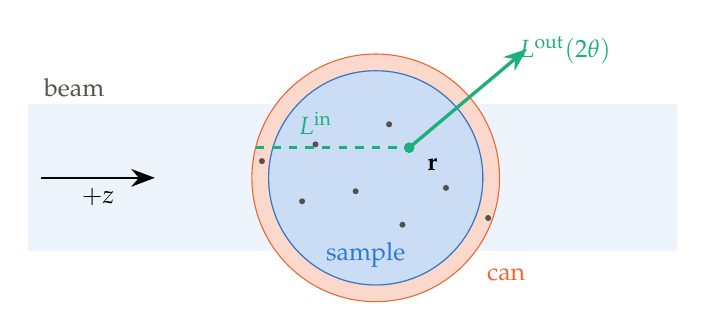
\begin{tikzpicture}[scale=0.85]
  \fill[accent!8] (-5.2,-1.1) rectangle (4.5,1.1);
  \node[font=\small,color=ink2,anchor=west] at (-5.1,1.35) {beam};
  \draw[fill=accent!25,draw=accent] (0,0) circle (1.6);
  \draw[fill=accent2!25,draw=accent2] (0,0) circle (1.6) circle (1.85);
  \draw[fill=accent!25,draw=accent] (0,0) circle (1.6);
  \foreach \p in {(-0.9,0.5),(0.4,-0.7),(1.05,-0.15),(-0.3,-0.2),(-1.1,-0.35),(0.2,0.8),(1.68,-0.6),(-1.7,0.25)}
    \fill[ink2] \p circle (0.045);
  \fill[accent3] (0.5,0.45) circle (0.08);
  \draw[very thick,accent3,dashed] (-1.794,0.45) -- (0.5,0.45);  % from the outer surface (R = 1.85)
  \draw[very thick,accent3,-{Stealth[length=3mm]}] (0.5,0.45) -- ++(40:2.3);
  \draw[-{Stealth[length=3mm]},thick] (-5,0) -- (-3.3,0) node[midway,below,font=\small] {$+z$};
  \node[font=\small,accent3,anchor=south] at (-0.9,0.5) {$L^{\mathrm{in}}$};
  \node[font=\small,accent3,anchor=west] at (2.0,1.9) {$L^{\mathrm{out}}(\twotheta)$};
  \node[font=\small,anchor=west] at (0.62,0.2) {$\mathbf r$};
  \node[font=\small,accent2] at (1.95,-1.45) {can};
  \node[font=\small,accent] at (-0.15,-1.15) {sample};
\end{tikzpicture}
\caption{The direct method. Points (grey) are drawn uniformly in the volume lit by the beam and sorted by layer. For each point the incident path
(dashed, followed backwards from the point) and the outgoing path towards the detector are computed exactly; the point contributes the weight
$\exp[-\sum\mu(L^{\mathrm{in}}+L^{\mathrm{out}})]$.}
\label{fig:direct-sketch}
\end{figure}

\begin{enumerate}
  \item \textbf{Points.} $(x,y)$ is drawn from the beam profile (\code{sample_beam_point}) and $z$ uniformly over the extent of the sample along the beam.
        \code{layer_of_points} tells in which material the point is (points outside the material or in the empty part of a partially filled layer
        are discarded). The drawing goes on until every layer with $\mu>0$ has \code{n_points} points, so a thin wall gets as many points as the
        sample.
  \item \textbf{Incident path.} It is computed exactly by following the beam \emph{backwards} from the point to the surface of the sample:
        \code{outgoing_path_lengths(points, -z)}. This works for side faces, empty headspace and tilted slabs without any special case.
  \item \textbf{Outgoing path.} \code{outgoing_path_lengths(points, detector direction)} for every angle, as in Chapter~\ref{ch:transmission}.
  \item \textbf{Weights.} Each point contributes $w=\exp[-\sum_i\mu_i(L^{\mathrm{in}}_i+L^{\mathrm{out}}_i)]$. $A_k$ is the mean of the weights of
        layer $k$, and its error is their standard deviation divided by $\sqrt{n_k}$.
  \item \textbf{Mean paths.} $\langle L_k\rangle$ is estimated from an independent set of uniform points: the fraction $p$ of draws that fall in any
        material, and, for each point in the material, the full path of its beam line in each layer (backwards plus forwards), giving
        $\langle L_k\rangle=\Delta z\,p\,\langle L_k(\text{line})/L_{\mathrm{tot}}(\text{line})\rangle$. This ``ratio'' estimate is unbiased and
        much less noisy for thin layers than counting the points in each layer.
\end{enumerate}
Only methods of the common sample interface are used, so the direct method works for every geometry of \mcams{} and for any new one.

\section{Calling the functions}

\begin{lstlisting}
from direct_attenuation import (attenuation_factors_direct, attenuation_factors_mc,
                                compare_results, plot_attenuation_factors)

ref = attenuation_factors_direct(sample, beam_width, beam_height, H=None, V=None,
                                 angles_deg=None, phi_deg=0.0, n_points=200_000, rng=None)
mc  = attenuation_factors_mc(sample, beam_width, beam_height, H=None, V=None,
                             angles_deg=None, phi_deg=0.0, n_particles=200_000,
                             n_batches=5, mean_path=ref.mean_path, rng=None)
print(compare_results(ref, mc))           # table: values, difference, z
plot_attenuation_factors([ref, mc])       # lines: ref; points: mc; lower panel: difference
\end{lstlisting}

Both functions return an \code{AttenuationResult}:
\begin{center}\small
\begin{tabular}{@{}>{\raggedright\arraybackslash}p{5.4cm}p{9.2cm}@{}}
  \toprule \textbf{Attribute or method} & \textbf{Content} \\ \midrule
  \code{factors[k]}, \code{errors[k]} & $A_k(\twotheta)$ and its statistical error (one standard deviation), one row per layer; NaN for a layer
                                        with $\mu=0$ or not reached by the beam \\
  \code{mean_path}, \code{mean_path_error} & $\langle L_k\rangle$ (mm) and its error \\
  \code{single_per_steradian()} & equation~(\ref{eq:single-sr}): singly scattered particles per incident particle per steradian \\
  \code{angles_deg}, \code{layer_names}, \code{layer(name)} & the angles; the names of the layers; index of a layer from its name \\
  \code{n_samples}, \code{seconds}, \code{method} & points per layer (direct) or particles (MC); run time; \code{"direct"} or \code{"monte carlo"} \\ \bottomrule
\end{tabular}
\end{center}
\begin{itemize}
  \item \code{n_points} is the number of points \emph{per layer}. The error of $A_k$ decreases as $1/\sqrt{\text{\code{n_points}}}$;
        $10^5$ points give 0.02--0.2\,\% for $\mu R\le 0.5$.
  \item \code{attenuation_factors_mc} sets the scatter fractions to 1 in a copy of the sample (they do not change $A_k$) and runs
        \code{transmission_by_last_layer} with \code{max_orders=1}, in \code{n_batches} independent runs that give the error bars. Give it
        \code{mean_path=ref.mean_path}, or the exact value when you know it (uniform beam lower than a cylindrical sample: area of the layer inside the
        beam divided by the beam width); otherwise it is estimated with \code{mean_material_paths}.
  \item \code{mean_material_paths(sample, beam_width, beam_height, H, V)} alone returns $\langle L_k\rangle$ and its error.
\end{itemize}

\pyexample{ex09_direct}

The thin V wall shows the difference between the methods: $10^5$ points give $A_{\mathrm V}$ to 0.15\,\% with the direct method, while
$2\times10^5$ Monte Carlo particles give 3\,\%.

\section{Using it as a reference for the Monte Carlo}

\subsection{Attenuation factors}

Run both functions with the same sample, beam and angles and look at \code{compare_results}: the column \code{z} is the difference in units of the
combined statistical error. If the two methods agree, $|z|$ is below 2 for most angles and layers and almost never above 3
(Figure~\ref{fig:direct-vs-mc}). Remember that the Monte Carlo uses the same particles for all angles, so its errors at different angles are
correlated: a whole curve may be shifted by about one error bar.

\begin{figure}[ht]
  \centering
  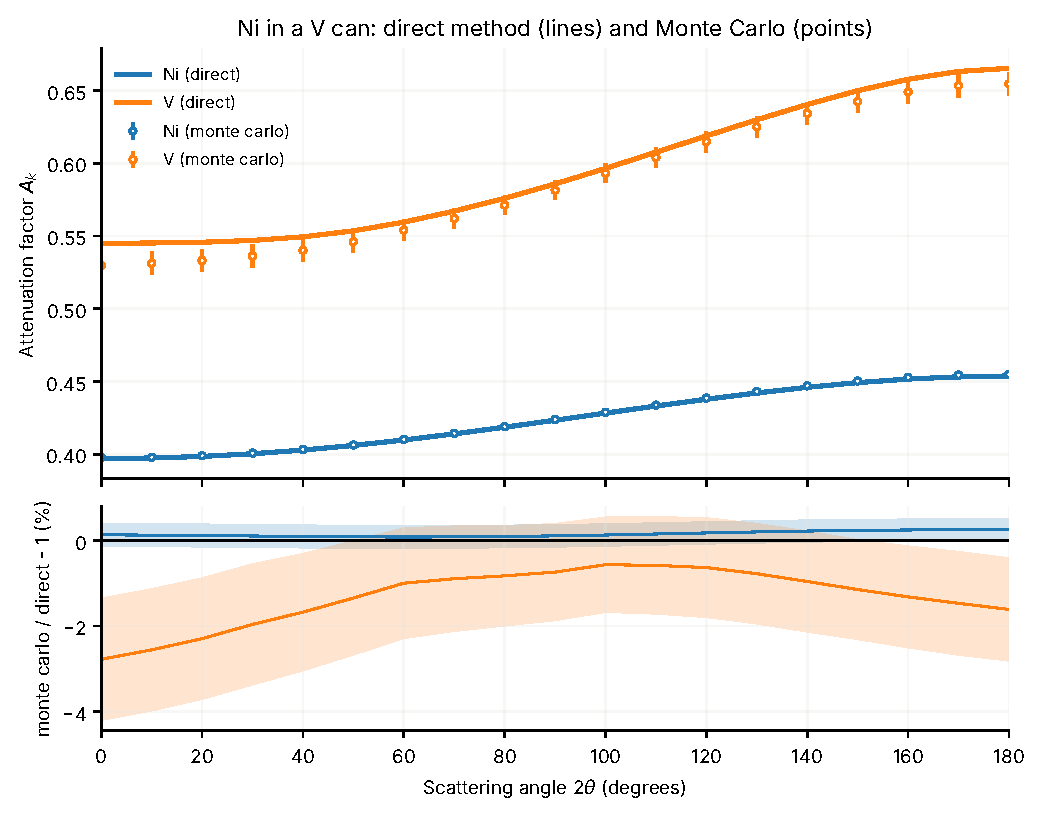
\includegraphics[width=0.82\textwidth]{fig_direct_vs_mc}
  \caption{Ni rod (6~mm) in a V can (0.2~mm), beam $15\times20$~mm: attenuation factors from the direct method (lines,
  $2\times10^5$ points per layer) and from the Monte Carlo (points, $20\times25\,000$ particles). Lower panel: relative difference with its
  $1\sigma$ band. The Monte Carlo error of the thin V wall is ten times larger than that of the direct method.}
  \label{fig:direct-vs-mc}
\end{figure}

\subsection{Single-scattering counts}

The particle-by-particle simulation of Chapter~\ref{ch:scattering} gives the singly scattered particles per steradian. Its expected value is
equation~(\ref{eq:single-sr}), which the direct method gives without noise. The detector direction of the direct method lies in the horizontal plane,
so use a narrow azimuth window in the simulation:
\begin{lstlisting}
from multiple_scattering import simulate_scattering_orders
res = simulate_scattering_orders(sample, 15, 20, n_particles=16_000_000,
                                 angle_edges_deg=np.arange(0, 181, 5.0),
                                 phi_deg=0.0, phi_halfwidth_deg=5.0, rng=7)
ref = attenuation_factors_direct(sample, 15, 20, angles_deg=res.angles_deg)
single_mc  = res.per_steradian(res.single)
single_ref = ref.single_per_steradian()          # the exact expectation
multiple   = res.per_steradian(res.multiple)     # Monte Carlo only
\end{lstlisting}

\begin{figure}[ht]
  \centering
  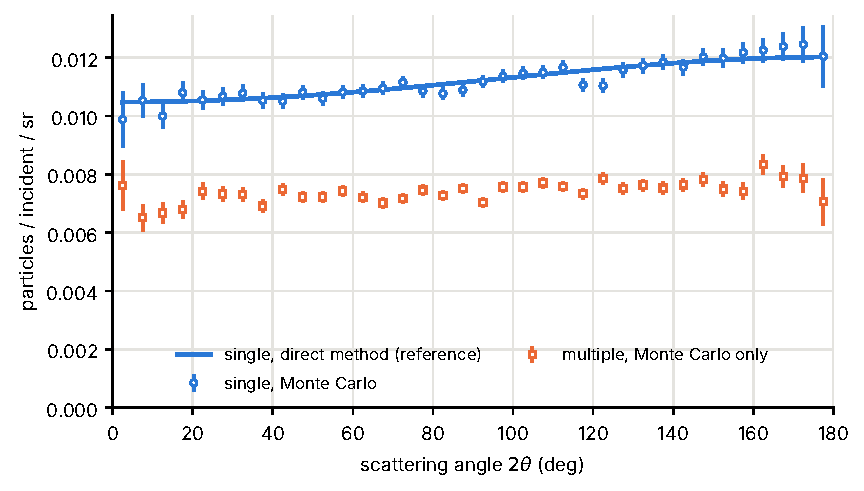
\includegraphics[width=0.78\textwidth]{fig_direct_orders}
  \caption{Same sample, $1.6\times10^7$ particles, azimuth window $\pm5^\circ$, $5^\circ$ bins. The single-scattering counts of the Monte Carlo
  (blue points) follow the direct reference (line): $\chi^2$ per bin 0.67, mean difference $-0.13\,\%$. The multiple scattering (orange) has
  no direct equivalent.}
  \label{fig:direct-orders}
\end{figure}

This comparison checks the whole random walk of the first event (beam, interaction point, scattering, direction, exit, counting) against an
independent calculation, and it separates in the measured signal the part that is known precisely (single) from the part that only the Monte Carlo
gives (multiple).

\section{Accuracy of the direct method}

The direct method has no discretisation: the paths are exact, and its only error is statistical and is computed with the result. It was checked
against exact or deterministic results (script \file{tools/direct\_method\_analysis.py}, part~1, $4\times10^5$ points per layer):

\begin{table}[H]
  \centering\small
  \begin{tabular}{@{}>{\raggedright\arraybackslash}p{6.2cm}ccccc@{}}
    \toprule \textbf{Case} & $\twotheta$ & \textbf{exact} & \textbf{direct} & \textbf{error} & $z$ \\ \midrule
    Slab, $\mu t=0.5$ (analytic) & $0^\circ$   & 0.60653 & 0.60653 & 0       & exact \\
                                                   & $60^\circ$  & 0.47730 & 0.47732 & 0.00011 & 0.15 \\
                                                   & $150^\circ$ & 0.61215 & 0.61212 & 0.00030 & $-0.12$ \\
    Same slab, fullness 0.5                        & $150^\circ$ & 0.61215 & 0.61265 & 0.00030 & 1.66 \\
    Ni + V can, 2~mm beam, $A_s$ (1D integral) & $0^\circ$ & 0.33956 & 0.33956 & 0.00001 & $-0.08$ \\
                                                   & $180^\circ$ & 0.40701 & 0.40752 & 0.00038 & 1.32 \\
    Furnace, $A_{h,sch}$ (fine grid) & $30^\circ$  & 0.75307 & 0.75316 & 0.00042 & 0.22 \\
                                                   & $150^\circ$ & 0.76136 & 0.76130 & 0.00044 & $-0.13$ \\ \bottomrule
  \end{tabular}
  \caption{Direct method against exact results: slab (analytic formulas for transmission and reflection), cylinder at $0^\circ$ and $180^\circ$
  (where the 2D integral reduces to a 1D integral, computed with \code{scipy.integrate.quad}) and a furnace at the angles where its factor has deep
  minima (deterministic midpoint grid of $40\times80\,000$ points, converged). $z$ = difference / error.}
  \label{tab:direct-exact}
\end{table}

All the differences are within the statistical error. The mean path is also correct: $\langle L\rangle=2.0000$~mm for the full slab of 2~mm and,
over 20 independent runs, $1.00003\pm0.00023$~mm for the slab filled to half the beam height (exact: 1~mm); the error quoted by the function
(0.00100 per run) agrees with the scatter of the runs (0.00104).

\section{Direct method and Monte Carlo compared}
\label{sec:direct-efficiency}

\subsection{Agreement}

Four samples were computed with both methods (part~2 of the script; direct: $2\times10^5$ points per layer, Monte Carlo: $20\times25\,000$
particles, 19 angles):

\begin{table}[H]
  \centering\small
  \begin{tabular}{@{}>{\raggedright\arraybackslash}p{4.4cm}lccccc@{}}
    \toprule \textbf{Sample} & \textbf{layer} & max$|z|$ & \textbf{mean diff.} & \textbf{err.\ direct} & \textbf{err.\ MC} & \textbf{FOM d/MC} \\ \midrule
    Ni in V can, 15~mm beam & Ni & 1.00 & $+0.15$\,\% & 0.09\,\% & 0.25\,\% & 1.7 \\
                                      & V  & 1.94 & $-1.32$\,\% & 0.11\,\% & 1.27\,\% & 30 \\
    same, 2~mm beam                   & Ni & 0.40 & $-0.02$\,\% & 0.08\,\% & 0.14\,\% & 2.0 \\
                                      & V  & 0.23 & $+0.13$\,\% & 0.10\,\% & 1.63\,\% & 148 \\
    Slab Al/Fe/Cu at $60^\circ$ & Al & 0.34 & $-0.13$\,\% & 0.02\,\% & 0.74\,\% & 580 \\
                                      & Fe & 0.86 & $-0.11$\,\% & 0.03\,\% & 0.27\,\% & 18 \\
                                      & Cu & 1.29 & $-0.27$\,\% & 0.02\,\% & 0.35\,\% & 55 \\
    Powder, $f=0.6$ & powder & 1.67 & $-0.41$\,\% & 0.12\,\% & 0.25\,\% & 1.3 \\
                                      & V  & 1.03 & $+0.84$\,\% & 0.11\,\% & 1.09\,\% & 30 \\ \bottomrule
  \end{tabular}
  \caption{Direct method against Monte Carlo (beam heights: 20~mm for the cylinders, 8~mm for the others; the powder fills its can to 0.6 of the beam height, in a Gaussian beam profile). max$|z|$: largest difference over the angles in units of the combined error; mean diff.: average
  of MC/direct\,$-1$ over the angles (correlated, see text); err.: mean relative error; FOM: figure of merit, defined below.}
  \label{tab:direct-mc}
\end{table}

The two methods agree within the statistics in every case, including the tilted slab, the partially filled container and the non-uniform beam
($|z|<2$ everywhere). The ``mean differences'' of about 1\,\% for the V walls are one correlated Monte Carlo error bar: the whole MC curve moves
together.

\subsection{Efficiency}

The \textbf{figure of merit} $\mathrm{FOM}=1/(\varepsilon^2\,t)$, with $\varepsilon$ the relative error and $t$ the run time, does not depend on the
number of samples: a method with ten times the FOM reaches the same precision ten times faster. Figure~\ref{fig:direct-fom} shows the ratio of the
FOM of the two methods for a single full cylinder ($R=3$~mm, beam $8\times20$~mm) as a function of its attenuation $\mu R$ (part~3 of the script):

\begin{figure}[ht]
  \centering
  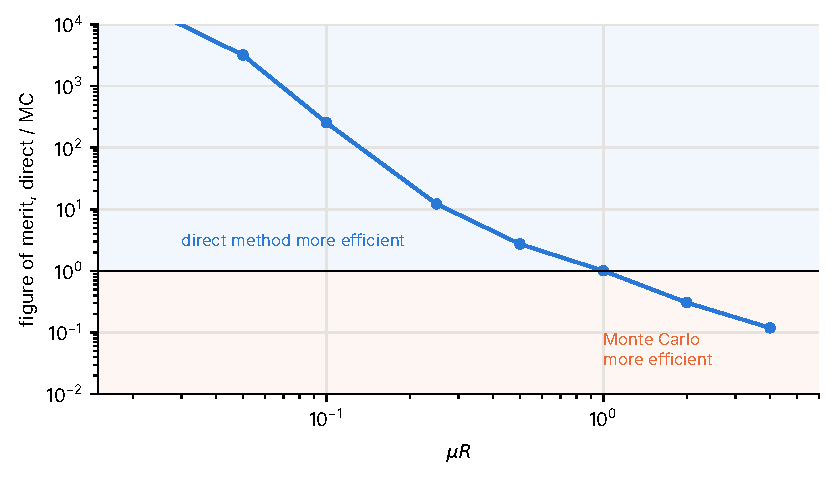
\includegraphics[width=0.72\textwidth]{fig_direct_fom}
  \caption{Figure of merit of the direct method divided by that of the Monte Carlo, for a cylinder of radius 3~mm, versus $\mu R$.}
  \label{fig:direct-fom}
\end{figure}

\begin{table}[H]
  \centering\small
  \begin{tabular}{@{}cccccc@{}}
    \toprule $\mu R$ & $A(90^\circ)$ & \textbf{interacting fraction} & \textbf{err. direct} & \textbf{err. MC} & \textbf{FOM direct/MC} \\ \midrule
    0.02 & 0.967 & 0.023 & 0.005\,\% & 0.91\,\% & 28\,000 \\
    0.05 & 0.919 & 0.056 & 0.011\,\% & 0.73\,\% & 2\,800 \\
    0.10 & 0.846 & 0.108 & 0.023\,\% & 0.39\,\% & 240 \\
    0.25 & 0.665 & 0.240 & 0.057\,\% & 0.19\,\% & 13 \\
    0.50 & 0.458 & 0.399 & 0.116\,\% & 0.16\,\% & 2.6 \\
    1.00 & 0.243 & 0.575 & 0.236\,\% & 0.16\,\% & 0.86 \\
    2.00 & 0.100 & 0.695 & 0.495\,\% & 0.17\,\% & 0.26 \\
    4.00 & 0.040 & 0.738 & 1.06\,\%  & 0.24\,\% & 0.12 \\ \bottomrule
  \end{tabular}
  \caption{Same comparison in numbers: direct method $10^5$ points, Monte Carlo $20\times25\,000$ particles, 5 angles. The agreement is within
  $|z|<1.6$ at all $\mu R$.}
  \label{tab:direct-fom}
\end{table}

\paragraph{Why.} The two methods treat the incident attenuation in opposite ways.
\begin{itemize}
  \item The \textbf{Monte Carlo} places its interaction points with the Beer--Lambert law: where the beam is strong. This is \emph{importance
        sampling} of the incident attenuation, and the only remaining randomness is the outgoing attenuation. Its weakness is that only the
        interacting fraction of the particles (third column) does any work: for $\mu R=0.02$, 98\,\% of them cross the sample and are wasted.
  \item The \textbf{direct method} uses every point, but weights it with the incident attenuation. When the attenuation is weak the weights are all
        close to one and the variance is tiny. When it is strong the weights span orders of magnitude (most points sit in the ``shadow'' and carry
        almost nothing), and a few points near the entrance surface dominate the mean.
\end{itemize}
The two are equally efficient near $\mu R\approx1$ (more precisely, when about half of the beam interacts in the layer).

\section{When to use which}

\begin{table}[H]
  \centering\small
  \begin{tabular}{@{}>{\raggedright\arraybackslash}p{7.4cm}>{\raggedright\arraybackslash}p{7.2cm}@{}}
    \toprule \textbf{Situation} & \textbf{Best tool} \\ \midrule
    Attenuation factors of containers, furnace and cryostat walls, thin layers, weakly absorbing samples ($\mu R\lesssim0.5$) &
      \textbf{direct method}: 10 to $10^4$ times faster at equal precision \\
    Attenuation factors of a typical sample, $\mu R\approx0.5$--1 & either; the direct method is simpler (no normalisation) \\
    Attenuation factors of strongly attenuating samples, $\mu R\gtrsim1$ & \textbf{Monte Carlo}: 4--8 times more efficient at $\mu R=2$--4 \\
    Multiple scattering, scattering orders, last layer of multiply scattered particles & \textbf{Monte Carlo only} \\
    Effect of the angular distribution of the scattering (Henyey--Greenstein, \dots) & \textbf{Monte Carlo only} (single attenuation does not
      depend on it) \\
    Histograms with bins and azimuth windows, total measured signal & \textbf{Monte Carlo}; the direct method gives the exact single part to compare \\
    Checking a Monte Carlo result, or a code such as CORRECT & \textbf{direct method} as reference \\ \bottomrule
  \end{tabular}
  \caption{Choosing between the direct method and the Monte Carlo.}
  \label{tab:direct-choice}
\end{table}

\begin{warn}[Limitations of the direct method]
\begin{itemize}
  \item \textbf{Single scattering only.} Nothing about the second and later scatterings: for multiple scattering, use the Monte Carlo
        (Chapters~\ref{ch:scattering} and~\ref{ch:lastlayer}).
  \item \textbf{Strong attenuation.} For $\mu R\gtrsim1$ its error grows quickly (1\,\% at $\mu R=4$ with $10^5$ points) and the Monte Carlo is more
        efficient. The result is still correct, only noisier.
  \item \textbf{Point detector.} The detector is a direction (in the horizontal plane for $\varphi=0$), as in Chapters~\ref{ch:transmission}
        and~\ref{ch:lastlayer}. To compare with the counts of Chapter~\ref{ch:scattering}, use a narrow azimuth window.
  \item \textbf{Isotropic scattering} in \code{single_per_steradian}; $A_k$ itself does not depend on the angular distribution.
  \item \textbf{Sampling volume.} Points are drawn in a box around the sample along the beam. For a strongly tilted, wide slab or a layer that
        fills a small part of that box, many draws are discarded; this costs time (drawing is cheap) but not accuracy. A layer that the beam does not
        reach gets NaN after \code{max_draws} draws.
  \item \textbf{Same physics as the Monte Carlo.} Straight paths, Beer--Lambert attenuation and the same geometry: the direct method checks the
        implementation and the statistics, not these common assumptions (Chapter~\ref{ch:limits}).
\end{itemize}
\end{warn}

\section{Reproducing the analysis}

\begin{lstlisting}[style=shell]
cd manual/tools
python direct_method_analysis.py          # parts 1-4, about 2.5 minutes
python direct_method_analysis.py 3        # only the efficiency study
\end{lstlisting}
The numbers are written to \file{tools/output/direct\_part1.txt} \dots{} \file{direct\_part4.txt} and the figures to \file{figures/fig\_direct\_*.pdf}.
The self-test \file{tests/test\_mcams.py} contains a short version of the checks (analytic slab, exact cylinder at $0^\circ$, mean paths, agreement
with the Monte Carlo).

\chapter{Preparing the layers from formula, density and cross sections}
\label{ch:builder}

\section{Purpose}

The simulations need, for every layer, the label, the thickness, the total linear attenuation coefficient $\mu$ and the scatter fraction. The module
\code{layer_builder.py} computes the last two from what is normally known about a material: its chemical formula, its density and its cross sections. Three small modules
cooperate: \code{formula.py} reads the formula, \code{nuclear_data.py} provides atomic masses and (optionally) tabulated cross sections, and
\code{layer_builder.py} does the calculation.

\section{The calculation}

\begin{enumerate}
  \item The formula gives the number of atoms of each species in one \emph{formula unit} (for instance one H$_2$O molecule) and so the molar mass $M$ (g/mol).
  \item The density $\rho$ (g/cm$^3$) gives the number of formula units per cm$^3$,
        \begin{equation} n=\frac{\rho\,N_A}{M},\qquad N_A=6.02214076\times10^{23}\ \mathrm{mol}^{-1}. \end{equation}
  \item The cross section of a formula unit is the sum of the cross sections of its atoms. The linear attenuation coefficients, in mm$^{-1}$, are
        \begin{equation}
          \mu_\mathrm{scat}=n\,\sigma_\mathrm{scat}\times10^{-24}\times0.1,\quad
          \mu_\mathrm{abs}=n\,\sigma_\mathrm{abs}\times10^{-24}\times0.1,\quad
          \mu=\mu_\mathrm{scat}+\mu_\mathrm{abs},
        \end{equation}
        with the cross sections in barn ($10^{-24}$~cm$^2$); the factor 0.1 converts cm$^{-1}$ into mm$^{-1}$.
  \item The scatter fraction is $\sigma_\mathrm{scat}/(\sigma_\mathrm{scat}+\sigma_\mathrm{abs})$.
\end{enumerate}

\section{Writing the formula: the notation}

Chemical formulas are read by \code{parse_formula}. The notation, which also covers isotopes, is summarised in Table~\ref{tab:notation}.

\begin{table}[ht]
  \centering\small
  \begin{tabular}{@{}p{4.6cm}p{4.2cm}p{5.4cm}@{}}
    \toprule \textbf{What} & \textbf{Write} & \textbf{Comment} \\ \midrule
    Natural element & \code{Fe}, \code{H2O}, \code{NH3}, \code{Fe2O3Na2Li} & capital letter, optional lower-case letter; the number after the symbol is the number of atoms \\
    Fractional amounts & \code{La0.7Sr0.3MnO3} & decimals are allowed \\
    \textbf{Isotope} & \code{[2H]2O}, \code{[56Fe]2O3}, \code{[10B]4C}, \code{H2[18O]} & mass number and symbol \textbf{inside square brackets} \\
    Deuterium, tritium & \code{D2O}, \code{T2O} & shorthands for \code{[2H]} and \code{[3H]} \\
    Groups & \code{Ca(OH)2}, \code{Al2(SO4)3} & round parentheses, may be nested \\
    Hydrates & \code{CuSO4*5H2O} & separator \code{*} (or the middle dot); the dot ``.'' is reserved for decimals \\
    Mixture of isotopes & \code{[6Li]0.5[7Li]0.5F} & list each isotope with its amount \\ \bottomrule
  \end{tabular}
  \caption{Notation of chemical formulas.}
  \label{tab:notation}
\end{table}

The brackets are the key of the proposal: a number placed \emph{before} a symbol would be ambiguous (\code{H22H} could mean H$_{22}$ and H, or H$_2$ and $^2$H).
Inside brackets there is no doubt, and a bracket can never be confused with a number of atoms or with a group. A formula cannot start with a number, and
the case of the letters matters (\code{CO} is carbon monoxide, \code{Co} is cobalt). Wrong formulas raise a \code{FormulaError} that points at the problem.
The function returns a dictionary \code{{Species: number of atoms}}; a \code{Species} is a natural element or an isotope. In the dictionaries that you give to the other
functions, a species is written like in the formula but without brackets: \code{"Fe"}, \code{"56Fe"}, \code{"D"} (or \code{"2H"}).

\section{Where the cross sections come from}

\begin{description}
  \item[A. Your values for the whole formula unit:] \code{sigma_scat=..., sigma_abs=...}, in barn per formula unit.
  \item[B. Your values per species:] \code{cross_sections={"Fe": (sigma_scat, sigma_abs), "D": (...)}}, in barn per atom, for some or all species.
  \item[C. Tabulated values] for the species that you did not give in B (package \code{periodictable}, see below).
\end{description}
If \code{sigma_scat} and \code{sigma_abs} are given, A is used for everything and B must not be given. Otherwise every species uses B if present and C if not.
Atomic masses come from \code{masses={"Fe": 55.845}} if given, otherwise from the tables.

{\sloppy\textbf{Tabulated data.} If the package \code{periodictable} is installed, \code{AtomicData} (module \code{nuclear_data.py}) uses it for atomic masses of
elements and isotopes and for the neutron cross sections (scattering = coherent + incoherent, and absorption) at the thermal velocity 2200~m/s
(wavelength 1.798~\AA)~\cite{sears,periodictable}. With \code{wavelength_A=...} the \emph{tabulated} absorption is scaled with the $1/v$ law (proportional to the
wavelength); this fails for strong resonances (Cd, Sm, Eu, Gd, \ldots). Your own values are never modified.
Without the package there is a small built-in table of atomic weights (and of the masses of some isotopes), but \textbf{no table of cross sections} on purpose:
a wrong number would silently give a wrong result; you then provide the values yourself, and a clear error message tells you how if you forget.
To use another database, give \code{data=} an object with the methods \code{mass(species)} and \code{neutron_xs(species)}.\par}

\section{Calling the functions}

\begin{lstlisting}
props = compute_layer_properties(label, thickness, formula, density,
                                 sigma_scat=None, sigma_abs=None,
                                 cross_sections=None, masses=None,
                                 wavelength_A=None, data=None)
layer = make_layer_tuple(...)          # same arguments; returns only the tuple
\end{lstlisting}
\code{compute_layer_properties} returns a \code{LayerProperties} with every intermediate value (molar mass, formula units per cm$^3$, $\mu_\mathrm{scat}$,
$\mu_\mathrm{abs}$, $\mu$, scatter fraction, origin of the cross sections); \code{props.summary()} prints them and \code{props.as_tuple()} gives
\code{(label, thickness, mu, scatter_fraction)}. \code{make_layer_tuple} returns directly that tuple, which can be put in the list of layers of any sample
(Chapter~\ref{ch:sample}). The thickness is in mm and, for the first layer of a cylinder, it is the diameter.

\pyexample{ex07_layer_builder}

The result for water, $\mu=0.565$~mm$^{-1}$ ($5.65$~cm$^{-1}$), agrees with the well-known value of about 5.6~cm$^{-1}$ for thermal neutrons.
The cross sections of heavy water and of aluminium in the example are illustrative.

\section{Using tabulated values}

With \code{periodictable} installed, no cross section needs to be given:
\begin{lstlisting}
iron = make_layer_tuple("Fe plate", 1.0, "Fe", 7.87)                    # all from tables
fe57 = make_layer_tuple("57Fe foil", 0.1, "[57Fe]", 7.87)               # an isotope
cold = make_layer_tuple("water", 2.0, "H2O", 1.0, wavelength_A=4.0)     # absorption at 4 Angstrom
mixed = make_layer_tuple("D2O", 6.0, "D2O", 1.107,
                         cross_sections={"D": (7.64, 0.000519)})        # D given, O from tables
\end{lstlisting}
\textbf{Note.} The adapter to \code{periodictable} was written from the documented interface of the package and tested here only against a stand-in object with the
same attributes; the first time you use it, run \code{python layer_builder.py} to check that the tabulated values are found (Appendix~\ref{app:trouble}).

\chapter{The main script}
\label{ch:main}

\section{What it does}

\code{run_simulation.py} runs the whole chain for a chosen geometry:
\begin{enumerate}
  \item builds the sample (slab, disc, cylinder or sphere) from the settings at the top of the file;
  \item computes the transmission versus $\twotheta$ (Chapter~\ref{ch:transmission});
  \item simulates the particles one by one to obtain total, single and multiple scattering (Chapter~\ref{ch:scattering});
  \item computes the transmission by layer of last scattering (Chapter~\ref{ch:lastlayer});
  \item \raggedright prints a summary and saves the plots, with the name of the geometry in the file names
        (\texttt{transmission\_slab.png}, \texttt{scattering\_orders\_cylinder.png}, \texttt{transmission\_by\_layer\_cylinder.png}, \ldots).
\end{enumerate}

\section{Choosing the geometry}

From the command line:
\begin{lstlisting}[style=shell]
python run_simulation.py --geometry slab
python run_simulation.py --geometry cylinder --particles 500000
python run_simulation.py --geometry slab --plane-angle 60
python run_simulation.py --geometry disc --plane-angle 45      # version 2.3
python run_simulation.py --geometry sphere                      # version 2.4
python run_simulation.py --geometry cylinder --no-show     # only save the plots
python run_simulation.py --geometry cylinder --fullness 0.5  # half-full container
python run_simulation.py --geometry cylinder --bottom -6 --height 5   # band -6..-1 mm
\end{lstlisting}
From Python or a notebook:
\begin{lstlisting}
from run_simulation import run_simulation
results = run_simulation("cylinder", n_particles=300000, show=False)
results["scattering"].single          # counts of single scattering per bin
results["by_layer"].transmission      # table (layer, angle)
\end{lstlisting}
The options are summarised in Table~\ref{tab:cli}.

\begin{table}[ht]
  \centering\small
  \begin{tabular}{@{}p{4.2cm}p{10.4cm}@{}}
    \toprule \textbf{Option} & \textbf{Meaning} \\ \midrule
    \code{--geometry} & \code{slab}, \code{disc}, \code{cylinder} or \code{sphere} (the default is set by \code{DEFAULT_GEOMETRY} in the file). \\
    \code{--plane-angle} & Slab and disc: angle between the beam and the plane of the sample, in degrees (default 90). \\
    \code{--particles} & Number of particles of the single/multiple scattering simulation (default 500000). The transmission curves use one tenth of that number. \\
    \code{--no-show} & Do not open plot windows; only save the PNG files. \\
    \code{--bottom}, \code{--height} & Version 2.2: band of the material of the layers listed in \code{CONTENT_LAYERS}, from \code{bottom} to \code{bottom + height}, in mm from the centre of the beam; either may be omitted (bottom or top of the sample) (Chapter~\ref{ch:partial}). \\
    \code{--fullness} & Version 2.0: fullness of the layers listed in \code{CONTENT_LAYERS} (fraction of the beam height covered by their material, from the bottom of the sample); default: full. Not together with \code{--bottom}/\code{--height}. \\ \bottomrule
  \end{tabular}
  \caption{Command-line options of \texttt{run\_simulation.py}.}
  \label{tab:cli}
\end{table}

\section{Using your own sample}

Edit the settings at the top of the file:
\begin{lstlisting}
SLAB_LAYERS = [("Al", 2.0, 0.020, 1.0),   # name, thickness (mm), mu (1/mm), scatter fraction
               ("Fe", 1.0, 0.250, 0.6),
               ("Cu", 0.5, 0.300, 0.5)]
SLAB_WIDTH, SLAB_HEIGHT = 20.0, 20.0

CYLINDER_LAYERS = [("Fe", 6.0, 0.250, 0.6),   # first thickness = DIAMETER
                   ("Al", 1.0, 0.020, 1.0),
                   ("Cu", 0.5, 0.300, 0.5)]
CYLINDER_HEIGHT = 20.0

DISC_LAYERS = [("Al", 2.0, 0.020, 1.0),       # front face to the back, as the slab
               ("Fe", 1.0, 0.250, 0.6),
               ("Cu", 0.5, 0.300, 0.5)]
DISC_DIAMETER = 20.0                          # the disc is centred on the beam

SPHERE_LAYERS = [("Fe", 6.0, 0.250, 0.6),     # first thickness = DIAMETER
                 ("Al", 1.0, 0.020, 1.0),     # then radial thicknesses
                 ("Cu", 0.5, 0.300, 0.5)]     # centred on the beam

BEAM_WIDTH, BEAM_HEIGHT = 8.0, 8.0

SAMPLE_Y_BOTTOM = None                        # bottom of the sample; None = centred
CONTENT_LAYERS = {"slab": ["Fe"], "cylinder": ["Fe"], "disc": ["Fe"],
                  "sphere": ["Fe"]}           # used by --bottom/--height/--fullness
\end{lstlisting}
The tuples can be written by hand or produced with \code{make_layer_tuple} (Chapter~\ref{ch:builder}); a fifth element gives the fill
height of a layer in mm (Chapter~\ref{ch:partial}). The layers of the slab and of the disc go from the front to the back; those of the
cylinder and of the sphere from the axis (centre) outwards. \code{SAMPLE_Y_BOTTOM} is not used by the disc and the sphere, which are
always centred on the beam. The values in the file are only illustrative.

\section{A recommended workflow}

\begin{enumerate}
  \item \raggedright Write the layers with \code{make_layer_tuple} (or by hand) and check them with \code{make_sample(...)}\allowbreak\code{.summary()}.
  \item Run \code{transmission_vs_angle} with 20\,000--50\,000 particles to see the attenuation as a function of the angle; it is fast.
  \item Run \code{simulate_scattering_orders} with $10^5$--$10^6$ particles to know how important the multiple scattering is.
  \item Use \code{transmission_by_last_layer} to find out which layer dominates the attenuation at each angle.
  \item Repeat with \code{rng=seed} to reproduce a result exactly, and with different seeds to see the statistical spread.
\end{enumerate}

\section{Computing time}

The times below were measured with $5\times10^4$ particles and 181 angles in the transmission by layer; the single/multiple scattering
simulation of $10^6$ particles takes of the order of tens of seconds. The cylinder is slower than the slab because every path is cut into segments.
\begin{center}\small
\begin{tabular}{@{}lcc@{}}
  \toprule & \textbf{slab} & \textbf{cylinder} \\ \midrule
  \code{transmission_by_last_layer}, $5\times10^4$ particles, 181 angles & 0.6~s & 3.5~s \\ \bottomrule
\end{tabular}
\end{center}

\chapter{Worked examples: the corrections of CORRECT with MCAMS}
\label{ch:correct}

\section{Goal of this chapter}

The program \textsc{correct} corrects diffraction data for attenuation and multiple scattering with analytical models: the
Paalman \& Pings factors for the attenuation and the Blech \& Averbach tables for the multiple scattering. This chapter shows how to
compute the same quantities with \mcams, keeping the scheme and the notation of \textsc{correct}, so that the Monte Carlo results can
replace the analytical ones in the usual correction chain. \mcams\ is more accurate where the analytical models are approximate:
narrow beams, furnaces and other sample environments, multiple scattering beyond second order, angle dependence of the multiple
scattering, partially filled containers, and geometries that \textsc{correct} does not have (discs, spheres).

Nothing in the package is changed. The chapter uses the public functions of \mcams\ and a small helper file,
\file{examples/correct\_tools.py} (listed in Appendix~\ref{app:correcttools}), which you can copy next to your own scripts. Five worked
examples follow: a cylinder, an annular sample between two tubes, a flat plate, a disc and a sphere, each one in a container and inside
a furnace.

\section{The notation of CORRECT}

A measurement with a sample in a container inside a heater (or any sample environment) needs three runs:
\begin{center}\small
\begin{tabular}{@{}lll@{}}
  \toprule \textbf{Run} & \textbf{What is in the beam} & \textbf{Measured intensity} \\ \midrule
  sample & sample + container + heater & $I_{sch}$ \\
  empty container & container + heater & $I_{ch}$ \\
  environment & heater only & $I_{h}$ \\ \bottomrule
\end{tabular}
\end{center}
Each measured intensity is the sum of the single scattering of its parts, each one attenuated by \emph{everything present in that run}:
\begin{align}
  I_{sch} &= A_{s,sch}\, I_s + A_{c,sch}\, I_c + A_{h,sch}\, I_h, \label{eq:Isch}\\
  I_{ch}  &= A_{c,ch}\, I_c + A_{h,ch}\, I_h, \label{eq:Ich}\\
  I_{h}   &= A_{h,h}\, I_h . \label{eq:Ih}
\end{align}
$I_s$, $I_c$ and $I_h$ are the \emph{unattenuated} single scattering of sample, container and heater; $A_{x,y}$ is the attenuation
factor of the particles scattered in the part $x$ when the parts $y$ are present. For example $A_{s,sch}$ is the factor of the
sample attenuated by sample, container and heater; $A_{c,ch}$ that of the container attenuated by container and heater. The equations
are solved from the bottom up (Paalman \& Pings):
\begin{equation}
  I_h = \frac{I_{h}}{A_{h,h}}, \qquad
  I_c = \frac{I_{ch} - A_{h,ch} I_h}{A_{c,ch}}, \qquad
  I_s = \frac{I_{sch} - A_{c,sch} I_c - A_{h,sch} I_h}{A_{s,sch}} .
  \label{eq:pp-chain}
\end{equation}
Six factors are needed, all functions of $\twotheta$: $A_{s,sch}$, $A_{c,sch}$, $A_{h,sch}$, $A_{c,ch}$, $A_{h,ch}$ and $A_{h,h}$.
Equations (\ref{eq:Isch})--(\ref{eq:Ih}) hold for single scattering; the measured intensities also contain multiple scattering,
which must be removed (Section~\ref{sec:correct-ms}).

\section{One geometry, three samples}

The three runs use the same container and the same heater, at the same place. In \mcams\ this is one list of layers, written once
for the complete assembly, in which every layer gets a \textbf{role}:
\begin{center}\small
\begin{tabular}{@{}cl@{}}
  \toprule \textbf{Role} & \textbf{Meaning} \\ \midrule
  \code{"s"} & sample \\
  \code{"c"} & container (one or several layers: the two walls of an annular can, the two windows of a flat cell) \\
  \code{"h"} & heater or sample environment (one or several layers) \\
  \code{"-"} & empty space: a gap, the vacuum of the furnace, an empty inner cylinder \\ \bottomrule
\end{tabular}
\end{center}
From this list three samples are built, with the same geometry:
\begin{itemize}
  \item \textbf{sch}: all the layers as given;
  \item \textbf{ch}: the layers of the sample are made empty ($\mu=0$);
  \item \textbf{h}: the layers of the sample and of the container are made empty.
\end{itemize}
Figure~\ref{fig:correctconfigs} shows the three samples of the two cylindrical cases of this chapter. In the helper file:
\begin{lstlisting}
from correct_tools import correct_samples
layers = [("Ni powder", 6.0, 0.180, 0.94),       # inner cylinder: diameter 6 mm
          ("V can",     0.2, 0.0459, 0.78),
          ("vacuum",   11.8, 0.0, 1.0),          # empty up to a radius of 15 mm
          ("V heater",  0.1, 0.0459, 0.78)]
roles  = ["s", "c", "-", "h"]
samples = correct_samples(lambda L: create_cylindrical_sample(40.0, L), layers, roles)
# samples["sch"], samples["ch"], samples["h"]
\end{lstlisting}
The first argument of \code{correct_samples} is any function that turns a list of layers into a sample, so the same code works for
every geometry: only that function changes.

\begin{figure}[H]
  \centering
  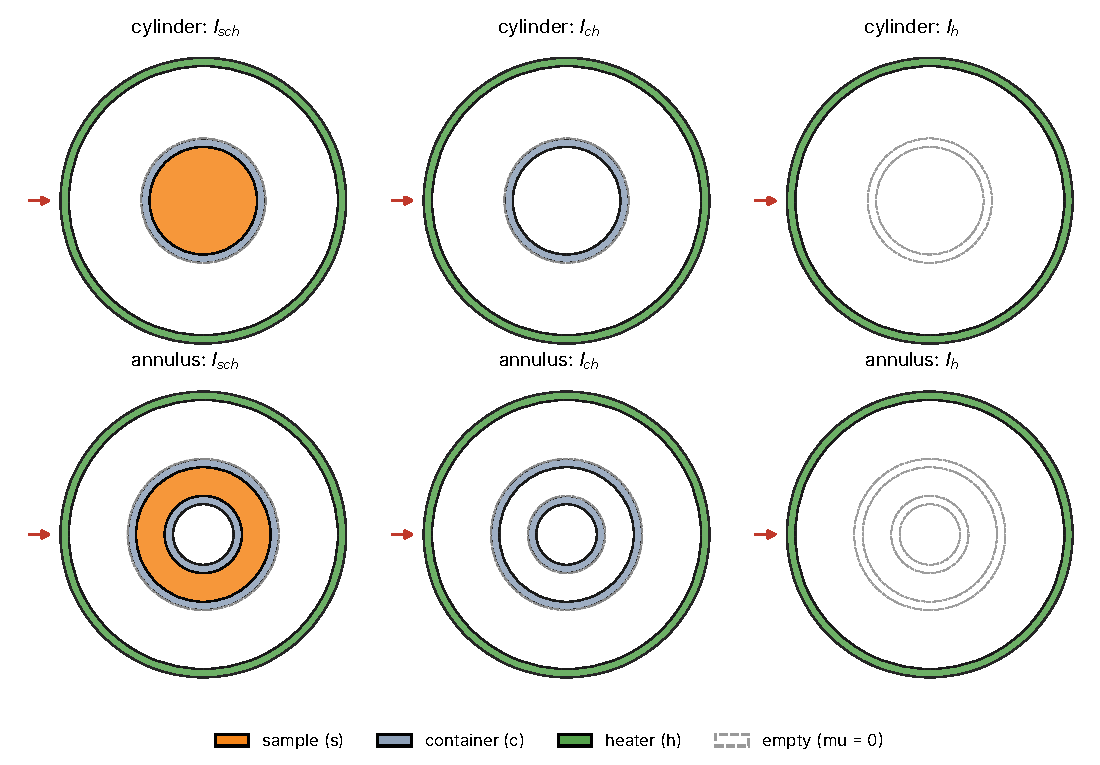
\includegraphics[width=0.92\textwidth]{fig_correct_configs}
  \caption{Top view of the three samples of the two cylindrical examples (radii not to scale). Top: sample in a can inside a
  furnace (Example~13). Bottom: annular sample between two tubes inside a furnace (Example~14). Dashed rings are empty layers
  ($\mu=0$): the geometry is the same in the three runs.}
  \label{fig:correctconfigs}
\end{figure}

\section{The attenuation factors}

The direct method (Chapter~\ref{ch:direct}) gives, for any sample, the single-scattering attenuation factor $A_k(\twotheta)$ of
every layer $k$: particles scattered once in layer $k$, attenuated on the way in and on the way out by all the layers of that sample.
So:
\begin{itemize}
  \item in the \textbf{sch} sample, the factor of the sample layer is $A_{s,sch}$, that of the container layers $A_{c,sch}$, that of the
        heater layers $A_{h,sch}$;
  \item in the \textbf{ch} sample, the container layers give $A_{c,ch}$ and the heater layers $A_{h,ch}$;
  \item in the \textbf{h} sample, the heater layers give $A_{h,h}$.
\end{itemize}
When a part has several layers, its factor is the average of the factors of its layers, weighted by how much each one scatters:
\begin{equation}
  A_{x,y} = \frac{\sum_{k\in x} w_k\, A_k}{\sum_{k\in x} w_k}, \qquad w_k = f_k\,\mu_k\,\langle L_k\rangle ,
  \label{eq:weights}
\end{equation}
where $f_k$ is the scatter fraction, $\mu_k$ the attenuation coefficient and $\langle L_k\rangle$ the mean path of the beam in the
layer. This is because the measured $I_c$ is the sum of the scattering of all the container layers, each one with its own
attenuation. The function \code{attenuation_factors} does all this:
\begin{lstlisting}
from correct_tools import attenuation_factors
A, err, mean_path = attenuation_factors(samples, roles, beam_width=10.0, beam_height=20.0,
                                        angles_deg=np.arange(0, 181, 10.0))
A["s,sch"], A["c,sch"], A["h,sch"], A["c,ch"], A["h,ch"], A["h,h"]    # arrays over 2theta
\end{lstlisting}
The direct method is used for the factors, rather than the first scatterings of the Monte Carlo, because it is much more precise
for thin layers (container walls, heater foils): every point contributes with its exact attenuation, instead of the few particles that
happen to interact in a 0.1~mm foil. Both give the same factors (Chapter~\ref{ch:direct}); \code{attenuation_factors_mc} can replace the
direct method in \code{attenuation_factors} if you want to check it.

\section{Single, multiple and total scattering}
\label{sec:correct-ms}

The Monte Carlo follows every particle through all its scatterings. For each of the three samples,
\code{transmission_by_last_layer} gives the scattering that reaches the detector at each angle, split into single ($S_y$) and
multiple ($M_y$) scattering and by the layer of the last scattering. Divided by $4\pi$ and by the number of incident particles these
are intensities per incident particle and per steradian (isotropic scattering). Their sum $S_y+M_y$ is what the detector measures.
The ratio
\begin{equation}
  \delta_y(\twotheta) = \frac{M_y}{S_y}, \qquad y = sch,\; ch,\; h,
\end{equation}
is the multiple scattering of the whole run: sample, container and heater together, including all the cross terms (a particle
scattered in the sample and then in the heater, and so on).
\begin{lstlisting}
from correct_tools import scattering
sc = scattering(samples, roles, 10.0, 20.0, angles, n_particles=200_000, n_batches=10)
sc["sch"]["single"], sc["sch"]["multiple"], sc["sch"]["total"], sc["sch"]["delta"]   # (mean, error)
sc["sch"]["single_by_part"]["c"]       # single scattering whose last event was in the container
\end{lstlisting}
The errors are the standard errors of the mean of the batches. Use at least 10 batches: with 4, for instance, the error estimate is
itself uncertain by a factor of about 2.

\paragraph{The correction.} With the philosophy of \textsc{correct}, but with the factors and the multiple scattering of \mcams:
\begin{enumerate}
  \item remove the multiple scattering from each measured intensity:
        $I_y^{(1)} = I_y / (1+\delta_y)$, for $y = sch,\,ch,\,h$;
  \item apply the Paalman \& Pings subtraction, eq.~(\ref{eq:pp-chain}), to $I_{sch}^{(1)}$, $I_{ch}^{(1)}$, $I_h^{(1)}$ with the
        six factors.
\end{enumerate}
\begin{lstlisting}
from correct_tools import correct_chain
I_s, I_c, I_h = correct_chain(I_sch_measured, I_ch_measured, I_h_measured, A,
                              delta={"sch": d_sch, "ch": d_ch, "h": d_h})
\end{lstlisting}
\textsc{correct} does step~2 and then subtracts an analytical $\delta$ from the corrected sample only, computed for an equivalent
homogeneous cylinder. Here every run is corrected with its own simulated multiple scattering, for the real geometry. This removes the
approximations of \textsc{correct} discussed in the comparison report: the empirical series for the higher orders, the neglect of the
angle dependence and of the material outside the beam, and the treatment of the container and environment.

\begin{note}[What delta assumes]
Like the Blech \& Averbach correction, $\delta_y$ is computed for \emph{isotropic} scattering in every layer (or for the angular
distribution given with \code{deflection_sampler}). For a sample with strong Bragg peaks or a strongly structured $S(Q)$ this is an
approximation, the same one made by \textsc{correct}. The attenuation factors do not depend on it.
\end{note}

\paragraph{The closure test.} Each example ends with a test of the whole procedure. The simulated totals $S_y+M_y$ are treated as
measurements and corrected with steps~1 and~2. The result must be the true unattenuated scattering of each part,
$I_x = \sum_{k\in x} f_k\mu_k\langle L_k\rangle/(4\pi)$ (function \code{unattenuated}). Because $\delta_y$ comes from the same
simulation, step~1 gives back exactly the simulated single scattering: the test checks the attenuation factors against the Monte
Carlo and the bookkeeping of the subtraction, not the multiple scattering itself. The last column shows what is left when the multiple
scattering is \emph{not} removed. The reference $I_x$ needs the mean paths $\langle L_k\rangle$, which are estimated by sampling; in a
furnace most of the volume is empty and this estimate has an error of a few 0.1\%, so it is averaged over 10 runs and its error is
included. The correction itself does not need $\langle L_k\rangle$.

\section{The helper functions}

\begin{fnbox}{correct\_samples(make, layers, roles, runs=("sch", "ch", "h"))}
The samples of the chosen runs (default the three of \textsc{correct}; \code{RUNS} for all seven) with the same geometry. \code{make(layers)} builds a sample (any geometry).
\code{configuration(layers, roles, measurement)} gives the layers of one of them.
\end{fnbox}
\begin{fnbox}{attenuation\_factors(samples, roles, beam\_width, beam\_height, angles\_deg, n\_points=100000, rng=1)}
The six factors (direct method), their errors, and the mean paths of the layers. Parts with several layers are combined with
eq.~(\ref{eq:weights}).
\end{fnbox}
\begin{fnbox}{scattering(samples, roles, beam\_width, beam\_height, angles\_deg, n\_particles=200000, n\_batches=10, rng=2)}
Single, multiple and total scattering and $\delta$ of the three runs, per incident particle and per steradian, with errors; also split by
the part of the last scattering, and the results of every batch.
\end{fnbox}
\begin{fnbox}{correct\_chain(I\_sch, I\_ch, I\_h, A, delta=None)}
Steps 1 and 2 above: returns the unattenuated $I_s$, $I_c$, $I_h$.
\end{fnbox}
\begin{fnbox}{unattenuated(sample, roles, beam\_width, beam\_height, n\_runs=10)}
True unattenuated single scattering of each part, and its relative error (reference of the closure test, absolute level).
\end{fnbox}
\begin{fnbox}{all\_attenuation\_factors(make, layers, roles, beam\_width, beam\_height, angles\_deg, n\_points=100000, rng=1)}
The 21 factors $A_{x,y}$ for the seven sets of parts (Section~\ref{sec:all-factors}).
\end{fnbox}
\begin{fnbox}{general\_correction(I, A, delta=None, rel\_err=None)}
Unattenuated $I_s$, $I_c$, $I_h$ from any set of runs by weighted least squares, with their errors and $\chi^2$.
\end{fnbox}
\begin{fnbox}{at\_angles(values, angles, new\_angles)}
Linear interpolation of a dict of curves (factors or $\delta$) onto other angles: the angles of the simulated runs, or of the data.
\end{fnbox}
\begin{fnbox}{print\_factors, print\_all\_factors, print\_scattering, print\_contributions, check\_closure, plot\_correct, plot\_all\_factors}
Tables of the results, the closure test, and the figure with the six factors and the three $\delta$.
\end{fnbox}

In all the examples the container and the heater are vanadium ($\mu = 0.0459$~mm$^{-1}$, scatter fraction 0.78), the sample is Ni powder
($\mu = 0.180$~mm$^{-1}$, scatter fraction 0.94, the values of the comparison report at $\lambda = 0.5$~\AA), and the beam is
$10\times20$~mm. The factors are computed every $1^\circ$ and the simulated runs every $2^\circ$ (Section~\ref{sec:grid}).

\subsection*{The angular grid}
\label{sec:grid}
The two calculations do not cost the same per angle. The direct method computes, for every point, the path towards each detector
angle; the Monte Carlo does it for every scattering event of every particle. For the furnace of Example~13 (one run):
\begin{center}\small
\begin{tabular}{@{}rrrr@{}}
  \toprule \textbf{step} & \textbf{angles} & \textbf{factors, direct method ($10^5$ points per layer)} & \textbf{$\delta$, Monte Carlo ($10\times2\times10^5$ particles)} \\ \midrule
  $10^\circ$ & 19 & 17~s & 22~s \\
  $5^\circ$ & 37 & 26~s & 38~s \\
  $2^\circ$ & 91 & 53~s & 83~s \\
  $1^\circ$ & 181 & 99~s & 169~s \\ \bottomrule
\end{tabular}
\end{center}
The factors have sharp features (the dips of the heater factors at $0^\circ$ and $180^\circ$, the collapse of plates near their grazing
angle), so they are computed every $1^\circ$. The multiple-scattering ratio $\delta$ varies slowly, so the Monte Carlo runs every $2^\circ$
and its results are interpolated (function \code{at_angles}, linear interpolation with \code{np.interp}) wherever they are needed on
the $1^\circ$ grid; the closure tests use the factors at the $2^\circ$ angles. With this choice an example with three runs takes 7--11~minutes
(22 for the annulus, which has six layers), and Example~18 (seven runs) about 20, on one processor core. Computing everything every $1^\circ$ would double the time
of the Monte Carlo for no visible gain.

% -------------------------------------------------------------------------
\section{Example 13: cylinder in a can inside a furnace}

Ni powder of 6~mm diameter in a V can (wall 0.2~mm), inside a cylindrical V heater of radius 15~mm (0.1~mm), all 40~mm high; the beam
($20$~mm high) only sees the middle of the sample.

\pyexample{ex13_correct_cylinder}

\begin{figure}[H]
  \centering
  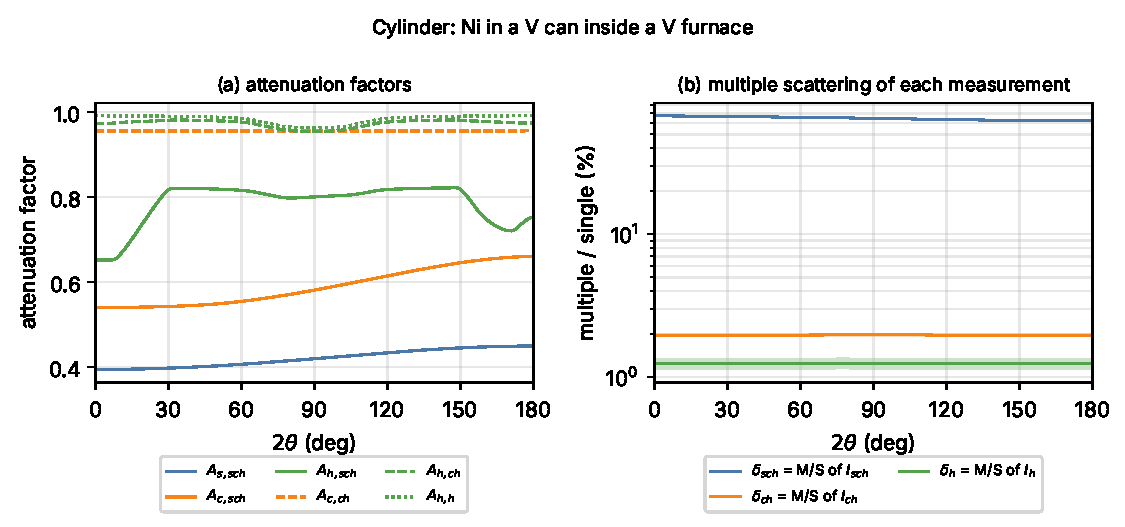
\includegraphics[width=\textwidth]{fig_correct_cylinder}
  \caption{Example 13. (a)~The six attenuation factors. (b)~$\delta=M/S$ of the three runs (log scale) (factors every $1^\circ$, $\delta$ every $2^\circ$ with its statistical error).}
  \label{fig:correctcyl}
\end{figure}

\begin{itemize}
  \item $A_{s,sch}$ goes from 0.394 at $0^\circ$ to 0.449 at $180^\circ$. $A_{c,sch}$ is lower than $A_{c,ch}$ (0.54--0.66 against 0.955):
        the particles scattered in the can cross the sample.
  \item $A_{h,sch}$ has dips at $0^\circ$ and $180^\circ$ (0.65 and 0.75 against about 0.82 elsewhere): there the particles
        scattered in the heater on the beam line cross the sample on their way to the detector. These are the dips that the
        parabolic interpolation of \textsc{correct} misses (comparison report).
  \item $A_{h,ch}$ and $A_{h,h}$ have a dip at $90^\circ$: particles scattered towards $90^\circ$ in the heater wall travel along it.
  \item The multiple scattering of the sample run is large, $\delta_{sch} = 0.67$--0.62 (it decreases with the angle). That of the
        empty can and of the heater is 2\% and 1.2\%.
  \item 94\% of the single scattering of $I_{sch}$ comes from the sample, 4\% from the can, 2--3\% from the heater; of the multiple
        scattering, 97\% ends in the sample.
  \item Closure: the sample is recovered within $0.1\% \pm 0.15\%$, the can and the heater within their statistical errors
        (about 0.9\%). Without the multiple-scattering correction the sample would be 66--71\% too high.
\end{itemize}

% -------------------------------------------------------------------------
\section{Example 14: annular sample between two tubes}

The sample fills the annulus between two coaxial V tubes. From the axis: an empty inner cylinder of 4~mm diameter (role \code{"-"}),
the inner V tube (0.2~mm), the Ni annulus (1.5~mm), the outer V tube (0.2~mm), vacuum, and the V heater at 15~mm. The two tubes
form the container: both have the role \code{"c"}, and their factors are combined with eq.~(\ref{eq:weights}).

\pyexample{ex14_correct_annulus}

\begin{figure}[H]
  \centering
  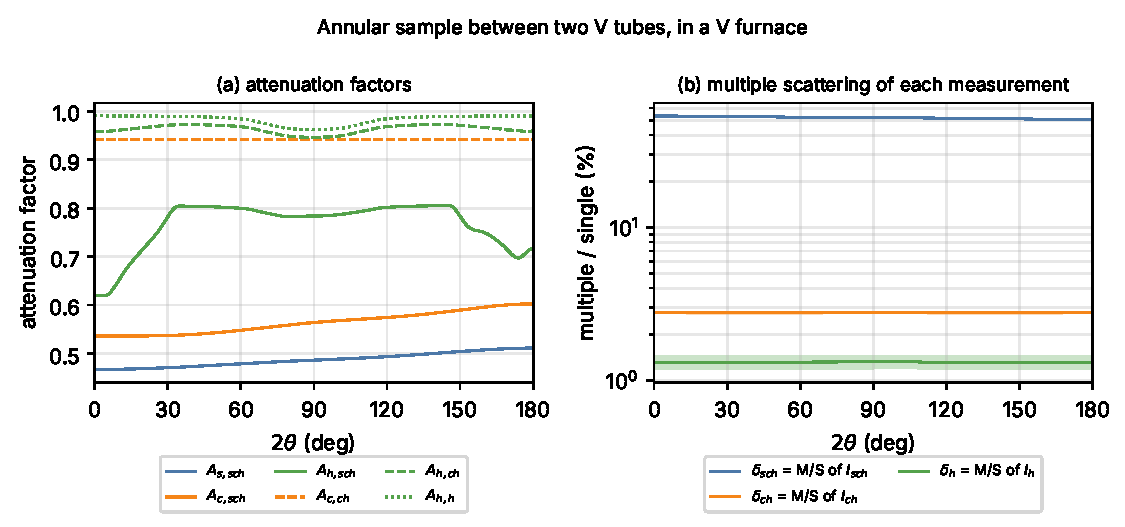
\includegraphics[width=\textwidth]{fig_correct_annulus}
  \caption{Example 14, annular sample. (a)~The six attenuation factors. (b)~$\delta$ of the three runs (factors every $1^\circ$, $\delta$ every $2^\circ$ with its statistical error).}
  \label{fig:correctann}
\end{figure}

\begin{itemize}
  \item The annular sample attenuates less than the full cylinder of Example~13 ($A_{s,sch}$ from 0.467 to 0.511) and has less multiple
        scattering ($\delta_{sch} = 0.53$--0.51), because it is thinner.
  \item The container now has two walls, with more material: $A_{c,ch} = 0.942$ and $\delta_{ch} = 2.8\%$; it gives 6\% of the single
        scattering of $I_{sch}$.
  \item Closure: sample within 0.1--0.3\% (errors 0.1\%), container and heater within their errors.
\end{itemize}
The same layout describes any coaxial assembly: a sample in a double-walled can, a cryostat with several shields (each shield is a
layer with the role \code{"h"}), a container inside a radiation shield, and so on.

% -------------------------------------------------------------------------
\section{Example 15: flat cell between flat heater windows (slab)}

A flat V cell (windows of 0.2~mm, 2~mm of Ni between them) between two flat V heater windows (0.1~mm), 10~mm in front of and behind
the cell, all $40\times40$~mm and perpendicular to the beam. The layers go from the front to the back; the two cell windows have the
role \code{"c"}, the two heater windows the role \code{"h"}. \code{z_front} puts the middle of the Ni on the rotation axis.

\pyexample{ex15_correct_slab}

\begin{figure}[H]
  \centering
  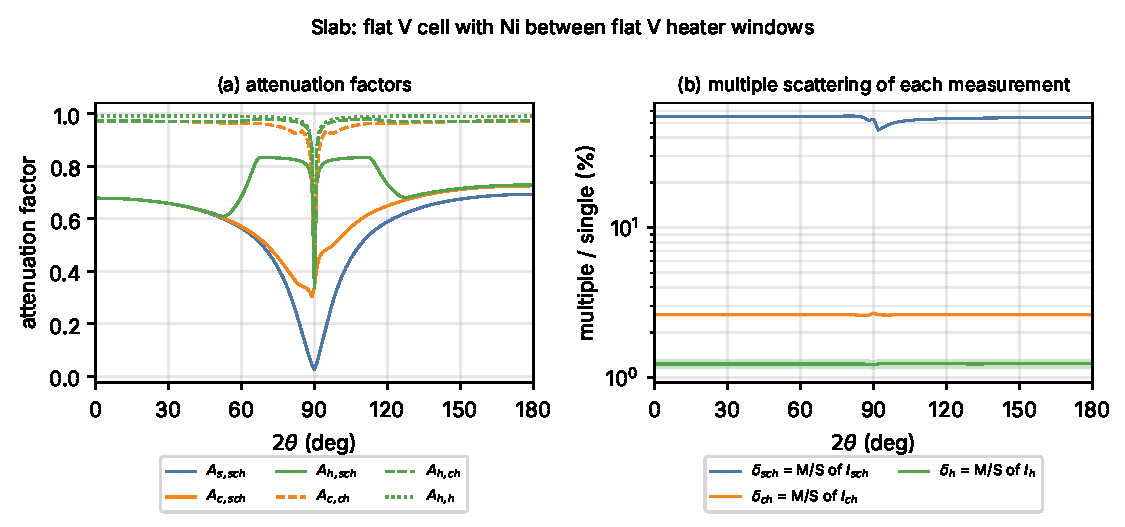
\includegraphics[width=\textwidth]{fig_correct_slab}
  \caption{Example 15, flat cell perpendicular to the beam. (a)~The six attenuation factors. (b)~$\delta$ of the three runs (factors every $1^\circ$, $\delta$ every $2^\circ$ with its statistical error).}
  \label{fig:correctslab}
\end{figure}

\begin{itemize}
  \item At $0^\circ$ every particle leaves along the beam line and crosses the whole stack, whatever layer it was scattered in: the three
        factors of $I_{sch}$ are equal, $\e^{-\sum\mu_k t_k} = 0.6787$. Likewise $A_{c,ch} = A_{h,ch} = \e^{-0.0459\times0.6} = 0.9728$
        and $A_{h,h} = \e^{-0.0459\times0.2} = 0.9909$. These are exact values, reproduced to the fourth decimal.
  \item At $90^\circ$ the scattered particles travel in the plane of the plate: the factors fall (0.026 for the sample) and this angle
        cannot be corrected in practice. Around it the factors change quickly; use a fine grid of angles there, or avoid it.
  \item $\delta_{sch} = 0.53$--0.55: a flat sample much wider than its thickness has a lot of multiple scattering in its plane.
        \textsc{correct} has no multiple-scattering correction for plates.
  \item Closure: sample within 0.1\% (0.3\% at $90^\circ$, error 0.5\%), container and heater within their errors.
\end{itemize}

% -------------------------------------------------------------------------
\section{Example 16: round cell between round heater windows (disc)}

The same stack as Example~15 with a circular section of 30~mm (Chapter~\ref{ch:disc}), rotated so that its plane makes $60^\circ$ with
the beam.

\pyexample{ex16_correct_disc}

\begin{figure}[H]
  \centering
  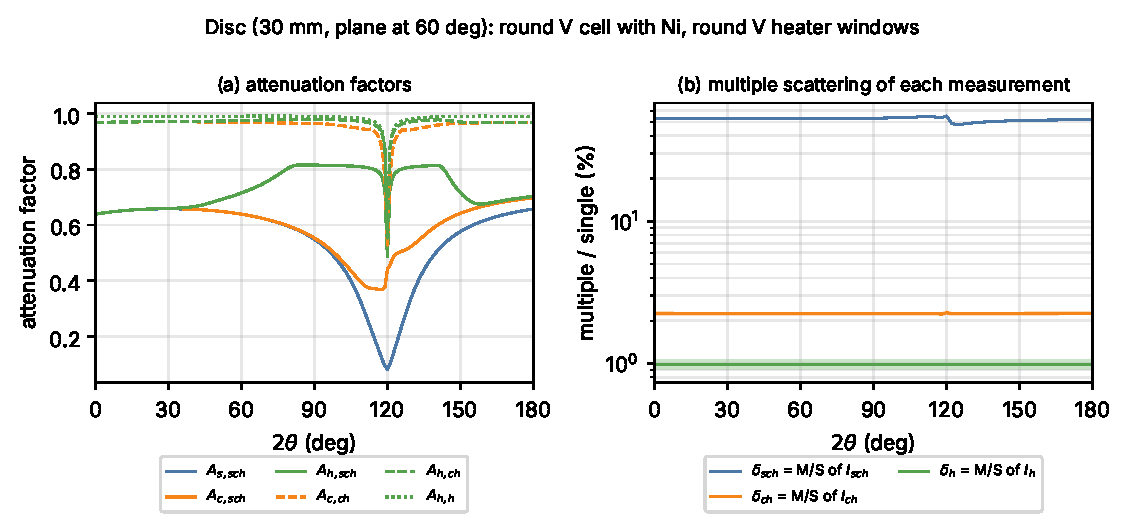
\includegraphics[width=\textwidth]{fig_correct_disc}
  \caption{Example 16, disc at $60^\circ$. (a)~The six attenuation factors. (b)~$\delta$ of the three runs (factors every $1^\circ$, $\delta$ every $2^\circ$ with its statistical error).}
  \label{fig:correctdisc}
\end{figure}

\begin{itemize}
  \item The grazing direction is now at $\twotheta = 180^\circ - 60^\circ = 120^\circ$, where the factors fall (0.082 for the sample).
  \item At $0^\circ$ the three factors of $I_{sch}$ are again equal (0.6393): the beam crosses the tilted stack along a path
        $1/\sin 60^\circ$ times longer, $\e^{-0.3875/0.866} = 0.6393$ ($\sum\mu_k t_k = 0.3875$). At $30^\circ$ the scattered particles leave along the normal of
        the disc, and the factors (0.659) equal those of the plate perpendicular to the beam at $30^\circ$ (Example~15): the incoming and
        outgoing paths are exchanged.
  \item Near the grazing angle the heater and the container give a larger share of $I_{sch}$ (26\% of the single scattering at
        $120^\circ$ against 6\% elsewhere): there the sample hides itself.
  \item Closure: all parts within their errors.
\end{itemize}

% -------------------------------------------------------------------------
\section{Example 17: sphere in a spherical container and heater}

A Ni sphere of 6~mm diameter in a V shell (0.2~mm), inside a spherical V heater of radius 15~mm (0.1~mm), all concentric
(Chapter~\ref{ch:sphere}).

\pyexample{ex17_correct_sphere}

\begin{figure}[H]
  \centering
  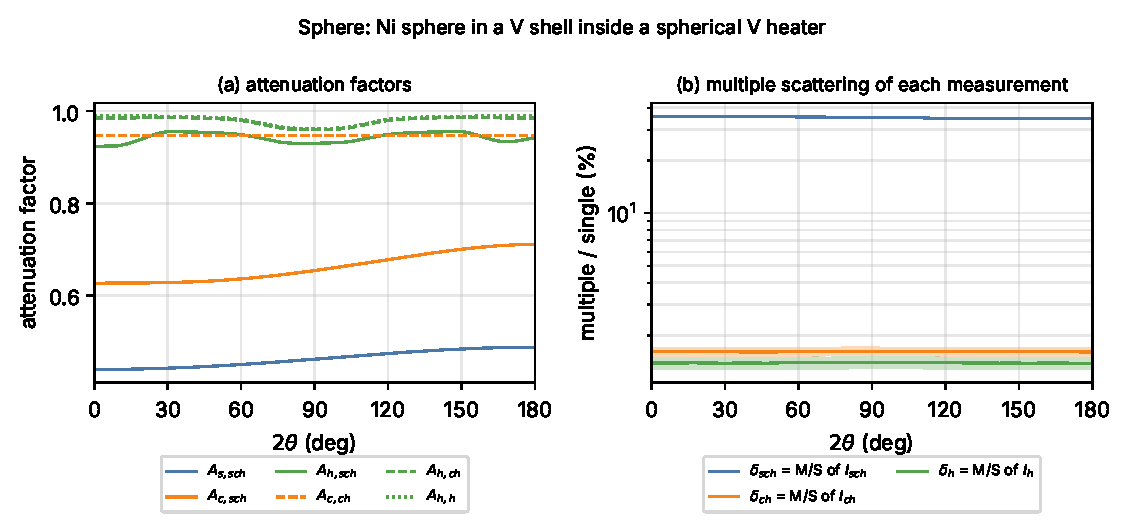
\includegraphics[width=\textwidth]{fig_correct_sphere}
  \caption{Example 17, sphere. (a)~The six attenuation factors. (b)~$\delta$ of the three runs (factors every $1^\circ$, $\delta$ every $2^\circ$ with its statistical error).}
  \label{fig:correctsphere}
\end{figure}

\begin{itemize}
  \item The sphere attenuates less than the cylinder of the same diameter in Example~13: $A_{s,sch} = 0.439$--0.487 against
        0.394--0.449, because its paths are shorter (Chapter~\ref{ch:sphere}). Its multiple scattering is also smaller,
        $\delta_{sch} = 0.36$--0.35 against 0.67--0.62.
  \item The sphere is small compared with the beam ($10\times20$~mm): most of the beam only crosses the heater, which gives 14\% of the
        single scattering of $I_{sch}$. The subtraction of the heater is important here.
  \item $A_{h,sch}$ is close to 1 (0.92--0.96): few of the particles scattered in the heater cross the small sample.
  \item Closure: sample within $0.4\% \pm 0.35\%$; the V shell, a very small volume, has a statistical error of 2\% in the simulated
        intensities (but its factors, from the direct method, are precise to 0.15\%).
\end{itemize}

% -------------------------------------------------------------------------
\section{All the factors $A_{x,y}$, and corrections with any set of runs}
\label{sec:all-factors}

A part $x$ (sample, container or heater) and a set $y$ of parts in the beam (one of the seven runs s, c, h, sc, sh, ch, sch) give
21 factors $A_{x,y}$:
\begin{center}\small
\begin{tabular}{@{}lccccccc@{}}
  \toprule & $y=$ s & c & h & sc & sh & ch & sch \\ \midrule
  $x=$ s & $A_{s,s}$ & $A_{s,c}^{*}$ & $A_{s,h}^{*}$ & $A_{s,sc}$ & $A_{s,sh}$ & $A_{s,ch}^{*}$ & $A_{s,sch}$ \\
  $x=$ c & $A_{c,s}^{*}$ & $A_{c,c}$ & $A_{c,h}^{*}$ & $A_{c,sc}$ & $A_{c,sh}^{*}$ & $A_{c,ch}$ & $A_{c,sch}$ \\
  $x=$ h & $A_{h,s}^{*}$ & $A_{h,c}^{*}$ & $A_{h,h}$ & $A_{h,sc}^{*}$ & $A_{h,sh}$ & $A_{h,ch}$ & $A_{h,sch}$ \\ \bottomrule
\end{tabular}
\end{center}
Do they all make sense? They fall into two groups.

\paragraph{$x$ in $y$: 12 correction factors.} The scattering part is in the beam and attenuates its own scattering. Each of these
factors is needed by some set of runs: the set decides which factors enter the equations
\begin{equation}
  I_y = \sum_{x\in y} A_{x,y}\, I_x \qquad\text{(one equation per run, single scattering)}.
  \label{eq:general}
\end{equation}
\begin{center}\small
\begin{tabular}{@{}>{\raggedright\arraybackslash}p{4.6cm}>{\raggedright\arraybackslash}p{2.0cm}>{\raggedright\arraybackslash}p{7.6cm}@{}}
  \toprule \textbf{Experiment} & \textbf{Runs} & \textbf{Factors} \\ \midrule
  sample in a container in a furnace (\textsc{correct}) & sch, ch, h & $A_{s,sch}$, $A_{c,sch}$, $A_{h,sch}$, $A_{c,ch}$, $A_{h,ch}$, $A_{h,h}$ \\
  sample in a container, no environment & sc, c & $A_{s,sc}$, $A_{c,sc}$, $A_{c,c}$ \\
  self-supporting sample in a furnace & sh, h & $A_{s,sh}$, $A_{h,sh}$, $A_{h,h}$ \\
  self-supporting sample, no environment & s & $A_{s,s}$ \\
  more runs than unknowns, e.g.\ sch, sc, ch, c, h & 5 runs & all the factors of these runs (least squares, below) \\ \bottomrule
\end{tabular}
\end{center}

\paragraph{$x$ not in $y$: 9 diagnostic factors} (marked $^{*}$). The scattering part is not in the beam, so it cannot scatter: these
factors never enter a correction. They can still be defined, as the attenuation of the scattering of $x$ by the \emph{other} parts only.
For example $A_{s,ch}$ is the attenuation, by the container and the heater, of particles scattered at the sample positions, as if the
sample were transparent. They answer two questions:
\begin{itemize}
  \item \emph{How is the attenuation shared between the parts?} For instance $A_{s,h}$ tells how much the heater alone attenuates the
        scattering of the sample.
  \item \emph{Can the factors be multiplied?} One is tempted to write $A_{s,sch}\approx A_{s,s}\,A_{s,c}\,A_{s,h}$ or
        $A_{s,sch}\approx A_{s,s}\,A_{s,ch}$. This is exact only if the attenuation by the other parts is the same for every point of
        $x$ (for instance for an infinite plate at $\twotheta=0$). In general it is not: the product of averages is not the average of
        the product. The diagnostic factors show how large the error is (Example~18).
\end{itemize}

\paragraph{How MCAMS computes the 21 factors.} For the factors with $x$ in $y$ nothing new is needed: the direct method on the sample of
run $y$. For $x$ not in $y$ the layers of $x$ are made \textbf{ghosts}: they keep their geometry but get a vanishing attenuation coefficient,
$\mu = 10^{-12}$~mm$^{-1}$ (\code{GHOST_MU}). The direct method then draws points in them, and their factor is the attenuation by the
parts that are present (a ghost attenuates by less than $10^{-10}$). In practice one sample per run $y$ is built, with the parts of $y$ real
and the others ghosts, and one direct-method run gives the factors of the three parts. Seven runs give the 21 factors:
\begin{lstlisting}
from correct_tools import all_attenuation_factors, print_all_factors
A, err = all_attenuation_factors(MAKE, layers, roles, 10.0, 20.0, angles)
A["s,sch"], A["s,sh"], A["c,sc"], A["s,ch"], ...       # 21 arrays over 2theta
\end{lstlisting}
Parts with several layers are combined with eq.~(\ref{eq:weights}), using the weights of the real layers.

\paragraph{Correcting with any set of runs.} Eq.~(\ref{eq:general}) is one linear equation per run, for the unknowns $I_s$, $I_c$,
$I_h$ that appear in the runs. With multiple scattering, $I_y$ is replaced by $I_y/(1+\delta_y)$. The function
\code{general_correction} solves these equations at every angle by weighted least squares (\code{np.linalg.lstsq}), each equation
divided by the error of its run:
\begin{lstlisting}
from correct_tools import general_correction
parts, errors, chi2 = general_correction(
    {"sch": I_sch, "sc": I_sc, "ch": I_ch, "c": I_c, "h": I_h},      # measured runs
    A, delta={"sch": d_sch, ...}, rel_err={"sch": e_sch, ...})
parts["s"], parts["c"], parts["h"]          # unattenuated I_s, I_c, I_h versus angle
\end{lstlisting}
\begin{itemize}
  \item With as many runs as unknowns, organised as in \textsc{correct} (sch, ch, h), the system is triangular and the least squares
        gives exactly the Paalman \& Pings chain (eq.~\ref{eq:pp-chain}).
  \item With more runs than unknowns, every part is determined by several runs: the statistical errors are smaller, and
        $\chi^2$ (the sum of the squared normalised residuals) measures the consistency of the runs. For $n_y$ runs and $n_x$ unknowns
        it should be about $n_y-n_x$. A much larger value means that something is wrong: a container not put back at the same place,
        a wrong $\mu$, a background not subtracted, a different beam.
  \item The errors of the solution come from the covariance of the least squares, $(M^\mathrm{T}WM)^{-1}$, where $M$ is the matrix of
        the factors and $W$ the weights.
\end{itemize}

% -------------------------------------------------------------------------
\section{Example 18: all the factors, and five sets of runs}

The assembly of Example~13 (Ni in a V can inside a V furnace). The script computes the 21 factors, tests the products, simulates the
seven runs (single and multiple scattering), and corrects them with five different sets of runs.

\pyexample{ex18_all_factors}

\begin{figure}[H]
  \centering
  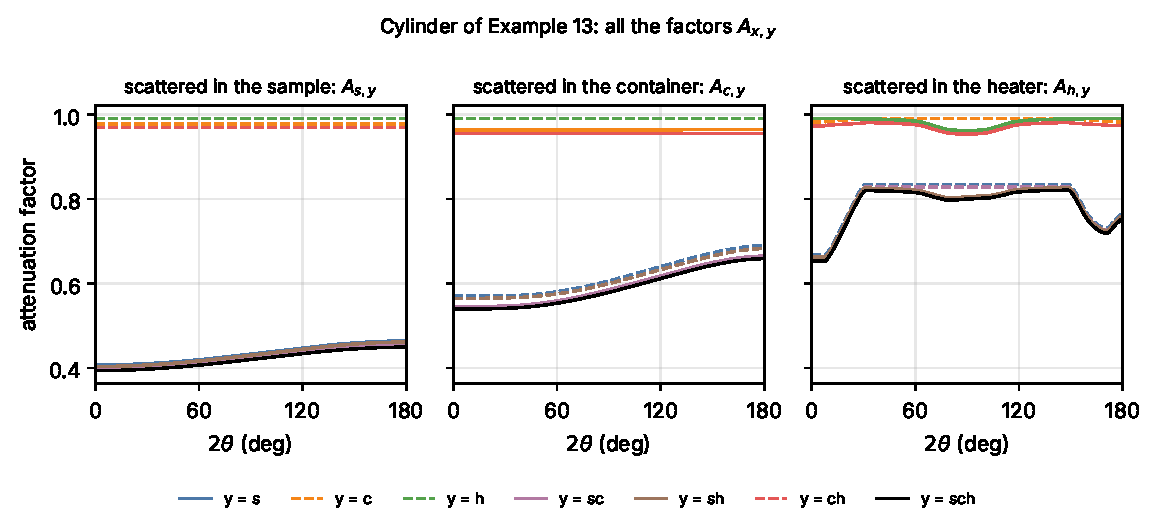
\includegraphics[width=\textwidth]{fig_all_factors_cylinder}
  \caption{Example 18: the 21 factors $A_{x,y}$ versus $\twotheta$ (every $1^\circ$), one panel per scattering part. Solid lines: $x$ in $y$
  (correction factors); dashed: $x$ not in $y$ (attenuation by the other parts only). The line styles of the legend are those of the
  first panel.}
  \label{fig:allfactors}
\end{figure}

\paragraph{The factors.}
\begin{itemize}
  \item The diagnostic factors are close to 1 for thin parts: the can alone attenuates the scattering of the sample by 2.2\%
        ($A_{s,c}=0.978$), the heater alone by 0.9\% ($A_{s,h}=0.991$, two crossings of 0.1~mm of V, $\e^{-0.0459\times0.2}$). The
        sample attenuates the scattering of the can by 30--43\% ($A_{c,s}=0.57$--0.69) and that of the heater most at $0^\circ$
        and $180^\circ$ ($A_{h,s}=0.67$ and 0.77, against 0.83 at $90^\circ$).
  \item \textbf{Products.} For the sample, $A_{s,s}A_{s,c}A_{s,h}$ agrees with $A_{s,sch}$ within 0.2\%, which is the statistical error of
        the comparison: the can and the heater attenuate almost uniformly over the sample. For the container and the heater the
        products are wrong by up to 0.8\% and 1\%: whether a particle scattered in the can or in the heater crosses the sample depends
        strongly on where it was scattered. The factors must therefore be computed for the complete assembly of each run, as done here,
        and not built as products.
  \item The multiple scattering depends little on the container and the heater: $\delta_s = 0.674$, $\delta_{sc}=0.681$,
        $\delta_{sch} = 0.675$ at $0^\circ$.
\end{itemize}

\paragraph{The corrections.} The sample is recovered within 0.1--0.4\% with every set of runs (errors 0.1--0.2\%), and the container and
heater within 1--3 standard errors. With the seven runs together the errors of all three parts are the smallest (0.09\% for the sample),
and $\chi^2$, 2.6--7.2 at the angles shown and 3.9 on average over the 91 angles, for 4 degrees of freedom, shows that the runs are
consistent. With sch, ch, h the least squares and the
Paalman \& Pings chain agree to $6\times10^{-16}$.

\begin{note}[Which factors do I need?]
Only those of the runs you measured: the 12 factors with $x$ in $y$ cover all the usual experiments, and the table above tells which
ones each experiment needs. The other 9 are for understanding the attenuation, not for correcting. If you measured more runs than
strictly needed (for example the empty container with and without the furnace), use them all with \code{general_correction}: you gain
statistics and a consistency test.
\end{note}

% -------------------------------------------------------------------------
\section{Using the factors with measured data}

\begin{enumerate}
  \item \textbf{Describe the assembly} with the real dimensions (mm) and the attenuation coefficients and scatter fractions of the
        materials at the wavelength of the experiment (Chapter~\ref{ch:builder}), and the real beam size and profile.
  \item \textbf{Choose the angles}: factors every $1^\circ$ (or every $2^\circ$ if time matters, with $1^\circ$ near the plane of a plate
        and the dips of the heater factors), $\delta$ every $2$--$5^\circ$ (Section~\ref{sec:grid}).
  \item \textbf{Compute} the factors with \code{attenuation_factors} and $\delta_y$ with \code{scattering}.
  \item \textbf{Interpolate} them onto the angles of the data: \code{at_angles(A, angles, theta_data)} and
        \code{at_angles(delta, angles_mc, theta_data)}.
  \item \textbf{Correct}: background subtraction and normalisation as usual, then \code{correct_chain}; the vanadium used for
        normalisation can be treated in the same way (a sample with its own environment, one more configuration).
\end{enumerate}

\begin{warn}[Statistics]
The factors of the direct method are precise (0.1--0.2\% with $10^5$ points per layer). The Monte Carlo intensities of thin parts
(walls, foils) have errors of 1--2\% with $2\times10^6$ incident particles, because few particles interact there. This is enough for
$\delta_{ch}$ and $\delta_h$, which are small (1--3\%), so their errors are negligible in the corrected data; for the sample,
$\delta_{sch}$ is known to a few 0.1\%. Increase \code{n_particles} or \code{n_batches} if needed.
\end{warn}

\chapter{Validation}
\label{ch:validation}

The calculations were checked against analytic results and against independent numerical methods. This chapter summarises the checks;
the figures and the numbers come from runs of the code with the settings indicated.

\section{Checks against exact results}

\begin{table}[ht]
  \centering\small
  \begin{tabular}{@{}p{7.2cm}p{7.5cm}@{}}
    \toprule \textbf{Check} & \textbf{Result} \\ \midrule
    Slab, single layer, oblique incidence: fraction of particles that interact for $\alpha=90^\circ,\,60^\circ,\,30^\circ$ & $0.5276,\,0.5797,\,0.7771$ against the Beer--Lambert values $0.5276,\,0.5794,\,0.7769$ \\
    Slab, transmission at $\twotheta=0$ for the same orientations & $0.6711,\,0.6287,\,0.4309$ against $0.6714,\,0.6287,\,0.4308$ \\
    Slab, general directions (four cases, both detector sides) & agreement with numerical integration within 0.0005 \\
    Slab, particles entering or leaving through side faces; next interaction of flying particles & brute-force ray stepping: 0 mismatches in 3000 and in 1500 random particles; positions within 0.0003~mm \\
    Cylinder, narrow beam through the axis & $0.7769$ against $1-\e^{-2\mu R}=0.7769$ \\
    Cylinder, beam as wide as the cylinder; beam wider than the cylinder & $0.6716$ against $0.672$; $0.3358$ against $0.336$ \\
    Cylinder, paths from the axis (horizontal, vertical, $45^\circ$, through the axis from an outer layer) & exact \\
    Cylinder, next interaction of random particles, including vertical directions & brute-force ray stepping: 0 mismatches in 1500; positions within 0.0003~mm \\
    Water, $\mu$ of thermal neutrons (Chapter~\ref{ch:builder}) & $5.65$~cm$^{-1}$, the known value is about $5.6$~cm$^{-1}$ \\ \bottomrule
  \end{tabular}
  \caption{Checks against exact results and against brute-force calculations.}
\end{table}

\section{Partially filled layers (version 2.0)}

The tracking was rewritten to include the levels of the material. The checks of Table~\ref{tab:valid-partial} were made; the
script \file{tests/test\_mcams.py} repeats those that do not need the old version.

\begin{table}[H]
  \centering\small
  \begin{tabular}{@{}>{\raggedright\arraybackslash}p{7.2cm}>{\raggedright\arraybackslash}p{7.5cm}@{}}
    \toprule \textbf{Check} & \textbf{Result} \\ \midrule
    Full layers: new code against version 1 with the same random seeds (slab at $90^\circ$, $60^\circ$, $125^\circ$; cylinder) & same particles interact; interaction points, outgoing paths and next interactions equal within $7\times10^{-15}$~mm \\
    Full layers: \code{transmission_vs_angle} and \code{simulate_scattering_orders}, same seeds & identical results (differences $\le 3\times10^{-16}$; identical counts) \\
    Partial layers: outgoing paths for 300 random points and directions, and for the directions $\pm x$, $\pm y$, $z$ & brute-force ray stepping (step $2\times10^{-4}$~mm): agreement within $3\times10^{-4}$~mm, both geometries \\
    Partial layers: next interaction of $2\times10^4$ random particles & optical depth to the new point equal to the random $\tau$ within $10^{-14}$; interaction if and only if $\tau$ is smaller than the optical depth to the exit; all points in material \\
    Slab, uniform beam, fullness $f=0.25,\,0.5,\,0.8,\,1$ & interacting fraction $f\,(1-\e^{-\mu t})$ within the statistical error ($4\times10^5$ particles) \\
    Cylinder, narrow beam through the axis, level inside the beam & $(7/8)(1-\e^{-2\mu R})$: $0.7948$ against $0.7956$ ($\pm0.0006$) \\
    Layer with fill height 0 & identical to a layer with $\mu=0$ \\ \bottomrule
  \end{tabular}
  \caption{Checks of the partially filled layers.}
  \label{tab:valid-partial}
\end{table}

\section{Layers with their own bottom and height (version 2.2)}

The material of a layer is now limited by two planes, $y=b_i$ and $y=t_i$, instead of one. The checks of Table~\ref{tab:valid-band}
were made; those that do not need the old version are in \file{tests/test\_mcams.py} (section~6).

\begin{table}[H]
  \centering\small
  \begin{tabular}{@{}>{\raggedright\arraybackslash}p{7.2cm}>{\raggedright\arraybackslash}p{7.5cm}@{}}
    \toprule \textbf{Check} & \textbf{Result} \\ \midrule
    Version 2.1 against 2.2, the same inputs and random seeds: transmission, scattering counts, transmission by layer, direct factors and mean paths for five samples (full and partially filled slabs and cylinders) & identical: largest difference 0.0 in all 30 quantities \\
    Slab, uniform beam, bands $(b,h) = (-6,5),\,(-2,5),\,(1,6),\,(-6,12),\,(5,3)$~mm in a 10~mm beam & interacting fraction $f\,(1-\e^{-\mu t})$ with $f$ from eq.~(\ref{eq:fullness-general}), within the statistical error \\
    Cylinder, narrow beam through the axis, band from $-1$ to $+3$~mm & $f\,(1-\e^{-2\mu R})$ within the statistical error \\
    \code{height=None}: envelope of the layers; \code{fill_levels}; \code{fill_height} $\equiv$ \code{bottom=y_bottom, height=fill_height} & exact \\
    \code{bottom}/\code{height} together with \code{fill_height} or \code{fullness} & refused with a clear message \\
    Direct method, mean path in a band covering a known part of the beam & $0.75$ of the full value, exact \\ \bottomrule
  \end{tabular}
  \caption{Checks of the layers with their own bottom and height.}
  \label{tab:valid-band}
\end{table}

The comparison with \textsc{pycorrect} (report \emph{pycorrect vs MCAMS}, chapter on partially filled samples) is a further test: the
fullness correction of \textsc{correct}, which is exact for single scattering when the can covers the whole beam and the beam is uniform,
applied to the intensities simulated by \mcams, gives back the true single scattering within 0.2--0.5\% (the statistical error) for
cylinders and flat cells, with the powder at the bottom, in the middle or at the top of the beam.

\section{Disc geometry (version 2.3)}

The disc reuses the path calculation of the slab with a different section, so it was checked both against exact results and
against the slab (Table~\ref{tab:valid-disc}). Section~7 of \file{tests/test\_mcams.py} contains these checks; sections~2 and~3 (paths
against brute-force ray stepping, next interaction) also run on two tilted discs with partially filled layers and bands. The test
script then ran 98 checks.

\begin{table}[H]
  \centering\small
  \begin{tabular}{@{}>{\raggedright\arraybackslash}p{7.2cm}>{\raggedright\arraybackslash}p{7.5cm}@{}}
    \toprule \textbf{Check} & \textbf{Result} \\ \midrule
    Slab and cylinder, version 2.2 against 2.3 (the slab code was reorganised), same inputs and seeds, five samples, 30 quantities & identical: largest difference 0.0 \\
    Outgoing paths in two discs ($\alpha=70^\circ$ and $125^\circ$, partial layers and bands), 300 random points and directions, and along $\pm x$, $\pm y$, $z$ & brute-force ray stepping: agreement within $2\times10^{-4}$~mm (the step) \\
    Next interaction in the same discs, $2\times10^4$ particles & optical depth to the new point equal to the random $\tau$ within $10^{-14}$; interaction if and only if $\tau$ is below the optical depth to the exit; all points in material \\
    Disc of 4000~mm against slab of $4000\times4000$~mm, $\alpha = 60^\circ$, same seeds & identical interaction points; identical outgoing paths for directions that leave through the faces \\
    Thin black disc (20~mm) in a $30\times30$~mm beam, $\alpha=90^\circ$ and $50^\circ$ & hit fraction 0.3486 and 0.2671 against the face area 0.3491 and 0.2674 \\
    Beam inside the disc, $\alpha=90^\circ$ and $60^\circ$ & interacting fraction $1-\e^{-\mu t/\sin\alpha}$ within the statistical error \\
    Disc of 10~mm in a $30\times30$~mm beam, normal incidence & $(\pi R^2/900)(1-\e^{-\mu t})$ within the statistical error \\
    Band from $-6$ to $0$~mm in an 8~mm beam; band larger than the disc & half of the Beer--Lambert value, \code{beam_fullness} 0.5; band cut at the rim \\
    Direct method, normal incidence: $A(0)$ and $A(90^\circ)$ & $A(0)=\e^{-\mu t}$ exactly; $A(90^\circ)$ equal to the separable integral over depth and face (0.21131 against 0.21150, within the error) \\
    Direct method against Monte Carlo, V/Ni/V disc at $\alpha=60^\circ$, three angles & $|z| < 4$ (largest 2.1) \\
    Fraction of a square beam that hits a thin disc, seven beam sizes, three orientations & agreement with \code{face_area_in_beam} within the statistical error (Figure~\ref{fig:discvalid}) \\ \bottomrule
  \end{tabular}
  \caption{Checks of the disc geometry.}
  \label{tab:valid-disc}
\end{table}

\section{Sphere geometry (version 2.4)}

The sphere reuses the segment calculation of the cylinder with spherical surfaces. Section~8 of \file{tests/test\_mcams.py} contains
the checks of Table~\ref{tab:valid-sphere}; sections~2 and~3 also run on two spheres, one with a partially filled layer and one with
bands. The test script now runs 124 checks.

\begin{table}[H]
  \centering\small
  \begin{tabular}{@{}>{\raggedright\arraybackslash}p{7.2cm}>{\raggedright\arraybackslash}p{7.5cm}@{}}
    \toprule \textbf{Check} & \textbf{Result} \\ \midrule
    Slab, disc and cylinder, version 2.3 against 2.4 (the cylinder code was reorganised), same inputs and seeds, 30 quantities & identical: largest difference 0.0 \\
    Outgoing paths in the two spheres, 300 random points and directions, and along $\pm x$, $\pm y$, $z$ & brute-force ray stepping: agreement within $4\times10^{-4}$~mm (twice the step) \\
    Next interaction in the same spheres, $2\times10^4$ particles & optical depth to the new point equal to the random $\tau$ within $10^{-14}$; interaction if and only if $\tau$ is below the optical depth to the exit; all points in material \\
    Points and directions rotated together by a random rotation (three full layers) & paths unchanged within $10^{-13}$~mm \\
    Pencil beam through the centre, $R=5$~mm, $\mu=0.2$~mm$^{-1}$ & $1-\e^{-2\mu R}$: 0.8636 against 0.8647 (within the error) \\
    Beam larger than the sphere ($12\times12$~mm) & $\frac{2\pi}{w_bh_b}\int_0^R(1-\e^{-2\mu u})\,u\,\deriv u$: 0.3834 against 0.3834 \\
    Black sphere in an $8\times8$~mm beam & hit fraction 0.9722 against \code{section_area_in_beam} 0.9717; $\pi R^2$ for a wide beam \\
    Half-filled sphere (up to $y=0$), vertical line beam & $\frac18\int_{-4}^{0}(1-\e^{-2\mu\sqrt{R^2-y^2}})\,\deriv y$: 0.4101 against 0.4115 (within the error); fullness 0.5 \\
    Direct method, $A(0)$ and mean path, beam larger than the sphere & $A(0) = \int L\e^{-\mu L}\deriv A/\int L\,\deriv A$: 0.24248 against 0.24249; mean path $\tfrac43\pi R^3/(w_bh_b)$ within the error \\
    Direct method against Monte Carlo, Ni sphere in a V shell, three angles & $|z|<4$ (largest 0.9) \\
    Factory: radii, vertical extent & \code{make_sample("sphere", ...)}: radii and $\pm R_\mathrm{out}$ as expected \\ \bottomrule
  \end{tabular}
  \caption{Checks of the sphere geometry.}
  \label{tab:valid-sphere}
\end{table}

\section{Worked examples in the notation of CORRECT (manual 2.5)}

Each example of Chapter~\ref{ch:correct} ends with a closure test: the simulated intensities of the three runs, corrected with the six
attenuation factors of the direct method and the simulated multiple scattering, give back the true unattenuated scattering of sample,
container and heater. For the five geometries the sample is recovered within 0.1--0.4\% (1--3 standard errors), and the container and
heater within their statistical errors (1--2\%). Some exact values are also reproduced: for a plate at $\twotheta=0$ all the factors of
a run equal $\e^{-\sum\mu_k t_k}$ (0.6787, 0.9728, 0.9909 in Example~15, and 0.6393 for the tilted disc of Example~16).

\section{All the factors and the least-squares correction (manual 2.6)}

In Example~18 the least-squares correction with the runs sch, ch, h reproduces the Paalman \& Pings chain to $6\times10^{-16}$; with four
other sets of runs (sc, c; sh, h; s; all seven) the sample is recovered within 0.1--0.4\% and $\chi^2$ is compatible with the number of
degrees of freedom. The diagnostic factors reproduce exact values ($A_{s,h} = \e^{-0.0459\times0.2} = 0.9909$ for the heater crossed
twice). A high-statistics run of the empty can ($2\times10^7$ particles) agrees with the direct method within $0.05\% \pm 0.19\%$.

\section{Consistency between the methods}

\begin{itemize}
  \item With all scatter fractions equal to 1, the \emph{single} transmission by layer of Chapter~\ref{ch:lastlayer}, averaged over the layers, reproduces the transmission of
        Chapter~\ref{ch:transmission} to rounding ($2\times10^{-15}$), for both geometries; the per-layer vectors agree with a direct calculation from the first
        interaction points to $3\times10^{-15}$.
  \item The particle-by-particle counts (Chapter~\ref{ch:scattering}) and the exact-direction estimate (Chapter~\ref{ch:lastlayer}) are two independent ways of
        computing the same quantity. Figure~\ref{fig:valid}(b) compares them for a tall two-layer cylinder with absorption, in a $\pm5^\circ$ azimuth window:
        they agree within the statistical error, for single and for multiple scattering.
  \item The bookkeeping closes: incident = no interaction + absorbed + exited (+ unfinished = 0), with and without absorption.
\end{itemize}

\begin{figure}[ht]
  \centering
  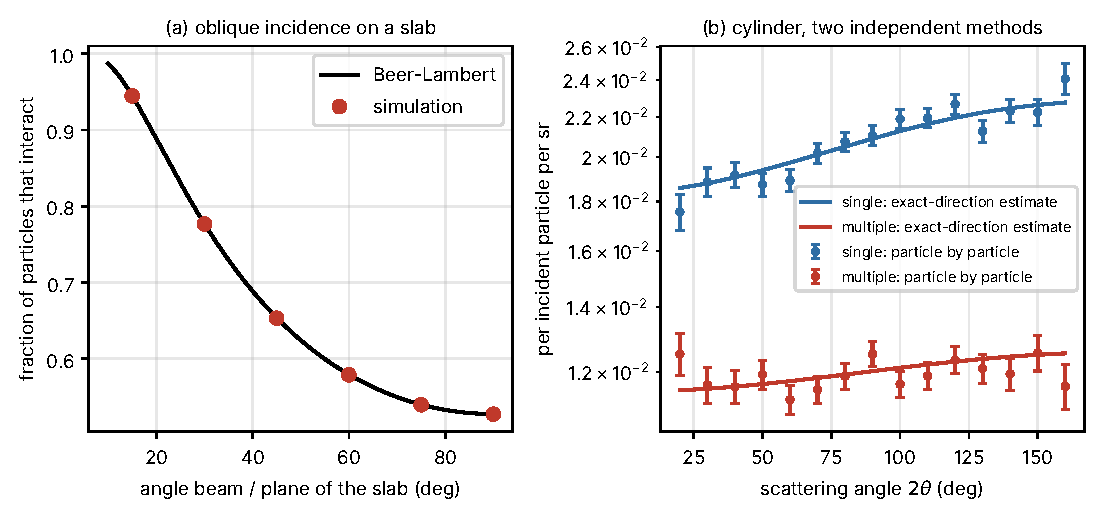
\includegraphics[width=\textwidth]{fig_validation}
  \caption{(a)~Fraction of particles that interact in a very wide single-layer slab ($\mu=0.25$~mm$^{-1}$, thickness 3~mm) versus the angle
  between the beam and the plane of the slab: simulation and Beer--Lambert law. (b)~Cylinder with absorption: single and multiple scattering per
  steradian, particle-by-particle counts (points with Poisson error bars) and exact-direction estimate (lines).}
  \label{fig:valid}
\end{figure}

\section{Formula reader and layer builder}

About twenty formulas were read correctly, including nested parentheses, hydrates, fractional amounts, isotopes and the shorthands D and T
(\code{Dy} is read as dysprosium and \code{Ti} as titanium, not as D or T followed by a letter); twelve incorrect formulas are rejected with a message. The
molar mass, the proportionality of $\mu$ with the density, the equality of per-atom and per-formula-unit inputs, the user overrides and the error messages were tested.

\section{Direct method (version 2.1)}

The direct method of Chapter~\ref{ch:direct} was checked against analytic results (slab in transmission and reflection, also partially
filled), against exact one-dimensional integrals (cylinder with a container and a narrow beam at $0^\circ$ and $180^\circ$) and against a converged
deterministic grid (furnace factors at $30^\circ$ and $150^\circ$): all within the statistical error (Table~\ref{tab:direct-exact}). It agrees with
the Monte Carlo within the statistics for slabs, tilted slabs, cylinders, partially filled containers and non-uniform beams
(Table~\ref{tab:direct-mc}), and its single-scattering intensity reproduces the single-scattering counts of the particle-by-particle simulation
($\chi^2$ per bin 0.67, Figure~\ref{fig:direct-orders}). The same checks, in a shorter form, are part of \file{tests/test\_mcams.py}.

\section{What has not been validated}

The adapter to the package \code{periodictable} has been tested only against a stand-in object with the same attributes (it was not installed in the
environment where the package was developed), so it should be checked on your system (Chapter~\ref{ch:builder}). No comparison with measured data has been made:
the example layers are illustrative.

\chapter{Assumptions, limits and possible extensions}
\label{ch:limits}

\section{Assumptions of the model}

\begin{itemize}
  \item \textbf{Interactions} are described by one total linear attenuation coefficient per layer; absorption and scattering are separated only by the
        scatter fraction. There is no energy (or wavelength) change in a scattering event.
  \item \textbf{Angular distribution} of one scattering event: isotropic by default, the same in all layers, independent of the incident direction apart from the
        deflection angle. A Henyey--Greenstein distribution or any user function can be used. Real materials, with coherent scattering, have angular patterns that depend
        on the material; they have to be provided by the user.
  \item \textbf{Transmission} is the pure attenuation along the path to the detector; the probability of scattering towards the detector (common factor) is not included
        in Chapters~\ref{ch:transmission} and~\ref{ch:lastlayer}. In Chapter~\ref{ch:scattering} it is included automatically, because the final directions are the result of the
        random scattering.
  \item \textbf{Detector}: the direction of the detector is exact (no angular width, no finite distance or size). The counting of Chapter~\ref{ch:scattering} uses bins in
        $\twotheta$ and, optionally, an azimuth window.
  \item \textbf{Geometry}: four shapes, slab (rectangular section), disc (circular section, centred on the beam, all layers of the same
        diameter), concentric cylinders and concentric spheres (centred on the beam). The sample has one height; the material of each layer lies between its own bottom and top, two flat horizontal surfaces,
        with empty space below and above (Chapter~\ref{ch:partial}). The cylinder axis passes through the centre of the instrument; the slab rotates
        about the vertical axis through the centre of its front face. There is no sample environment, no bottom or lid of the container, and no container other than the layers that you define.
  \item \textbf{Beam}: perfectly parallel, with independent horizontal and vertical profiles, centred on the axis. The sample can be moved vertically with \code{y_bottom}.
\end{itemize}

\section{Practical limits}

\begin{itemize}
  \item The direct method (Chapter~\ref{ch:direct}) is for single scattering only, and loses efficiency for $\mu R\gtrsim1$, where the
        Monte Carlo is better.
  \item Multiple scattering is followed up to \code{max_orders} scatterings per particle (default 200); \code{res.n_unfinished} tells how many particles were
        still inside (it should be 0).
  \item For the slab, a beam parallel to the plane of the sample is not allowed (the angle must be strictly between $0^\circ$ and $180^\circ$).
  \item Elements heavier than curium have no built-in mass: give it with \code{masses=}.
  \item Tabulated absorption cross sections scaled with $1/v$ are inaccurate near resonances.
\end{itemize}

\section{Ideas to extend the package}

\begin{itemize}
  \item \textbf{Direct method for strongly attenuating samples}: drawing the points along each beam line with the density $\mu\e^{-\tau}$
        (importance sampling) instead of uniformly would combine the advantages of the two methods of Chapter~\ref{ch:direct}.
  \item A \textbf{finite detector}: width, height and distance to the sample, counting the particles that reach it.
  \item An \textbf{angle-dependent cross section} for each material (for instance from a measured or computed structure factor), instead of an isotropic or
        Henyey--Greenstein distribution.
  \item \textbf{Other geometries}: write a new class that inherits from \code{LayeredSample} and implements the abstract methods (Table~\ref{tab:interface}).
        A flat sample with another convex section (an ellipse, a polygon) needs even less: a subclass of \code{SlabSample} that redefines
        \code{_section_interval} and \code{contains}, as the disc does (Section~\ref{sec:disc-algorithm}).
  \item \textbf{Sphere}: an offset centre; a neck or a stem (a vertical cylinder joined to the sphere); a hemisphere or other
        caps. A round shape whose layers are concentric needs only \code{_shell_interval}, \code{_radius_of} and
        \code{_outline_interval}, as the sphere (Section~\ref{sec:sphere-algorithm}): an ellipsoid or a horizontal cylinder are examples.
  \item \textbf{Disc}: an offset centre $(x_0,y_0)$; layers of different diameters (windows larger than the sample); a ring-shaped layer
        (a holder or a clamp around the sample).
  \item \textbf{X-ray attenuation}: only the data source changes (\code{nuclear_data.AtomicData} can be replaced through the argument \code{data=}).
  \item A \textbf{package structure} with an \code{__init__.py} file, so that the modules can be imported as a library.
  \item \textbf{Container bottom (base plate), lid or support}, a \textbf{gas} in the empty space, or a \textbf{meniscus}: they need horizontal layers or
        curved surfaces. A base plate is a horizontal disc (or slab) spanning several concentric layers; the material intervals (slab) and segments
        (cylinder) of Section~\ref{sec:partial-algorithm} can accommodate it with one more kind of region. For a two-axis detector in the
        horizontal plane a base plate below the beam only affects the multiple scattering.
  \item An \textbf{intensity-weighted fullness} for non-uniform beams, $\int V(y)\,\mathrm{d}y$ over the material divided by the same over the beam,
        as a method of the sample: this is the number to give to \textsc{correct} when the vertical profile is not flat.
\end{itemize}


\appendix
% ---------------------------------------------------------------------
% GENERATED by tools/make_api_appendix.py: do not edit by hand,
% run the script again after changing the code.
% ---------------------------------------------------------------------
\chapter{Reference of classes, functions and methods}
\label{app:api}

This appendix lists, module by module, every class, function and method of the package, with the signature and a one-sentence description taken from the docstrings. Methods are written as \code{Class.method(arguments)}. Names beginning with an underscore are internal helpers, listed for completeness. The full explanation of each item is in its docstring and in the chapters of this manual.

\section{\texorpdfstring{\texttt{beam.py}}{beam.py}: Incident beam}
\label{app:api:beam}
Where do the particles of a rectangular incident beam start?

\begin{longtable}{@{}p{1.75cm}p{6.35cm}p{6.45cm}@{}}
\toprule \textbf{Kind} & \textbf{Name and arguments} & \textbf{What it does} \\ \midrule \endhead
\small function & \raggedright\arraybackslash\small \texttt{\_\allowbreak{}sample\_\allowbreak{}1d(length, profile, n, rng, n\_\allowbreak{}grid=2001)} & \raggedright\arraybackslash\small Draw \texttt{n} random positions in [-length/2, +length/2] distributed according to \texttt{profile}. \emph{(internal)} \\
\small function & \raggedright\arraybackslash\small \texttt{sample\_\allowbreak{}beam\_\allowbreak{}point(width, height, H=None, V=None, n=1, rng=None)} & \raggedright\arraybackslash\small Pick the (x, y) point(s) in the beam rectangle where particle(s) start. \\
\small function & \raggedright\arraybackslash\small \texttt{start\_\allowbreak{}position(width, height, H=None, V=None, z0=0.\allowbreak{}0, rng=None)} & \raggedright\arraybackslash\small Convenience wrapper: one particle, returned as a 3D point (x, y, z0) together with its direction of flight (0, 0, 1), i.e. along +z. \\
\bottomrule
\end{longtable}

\section{\texorpdfstring{\texttt{sample\_base.py}}{sample_base.py}: Common ingredients of all samples}
\label{app:api:sample_base}
Ingredients shared by ALL sample geometries of MCAMS.

\begin{longtable}{@{}p{1.75cm}p{6.35cm}p{6.45cm}@{}}
\toprule \textbf{Kind} & \textbf{Name and arguments} & \textbf{What it does} \\ \midrule \endhead
\small dataclass & \raggedright\arraybackslash\small \texttt{Layer(name: str, thickness: float, mu: float, scatter\_\allowbreak{}fraction: float = 1.\allowbreak{}0, fill\_\allowbreak{}height: Optional[float] = None, fullness: Optional[float] = None, bottom: Optional[float] = None, height: Optional[float] = None)} & \raggedright\arraybackslash\small One layer of the sample. \\
\small property & \raggedright\arraybackslash\small \texttt{Layer.\allowbreak{}is\_\allowbreak{}partial} & \raggedright\arraybackslash\small True if the layer was declared with a limited vertical extent (bottom, height, fill\_height, or fullness < 1). \\
\small function & \raggedright\arraybackslash\small \texttt{make\_\allowbreak{}layer(item)} & \raggedright\arraybackslash\small Turn one item of a list of layers into a \texttt{Layer}. \\
\small function & \raggedright\arraybackslash\small \texttt{scattered\_\allowbreak{}direction(two\_\allowbreak{}theta\_\allowbreak{}deg, phi\_\allowbreak{}deg=0.\allowbreak{}0)} & \raggedright\arraybackslash\small Unit vector (LAB frame) of a particle scattered by \texttt{two\_\allowbreak{}theta\_\allowbreak{}deg} from the beam direction +z. \\
\small class & \raggedright\arraybackslash\small \texttt{LayeredSample(ABC)} & \raggedright\arraybackslash\small Abstract base class of the layered samples (slab, cylinder, ...). \\
\small init & \raggedright\arraybackslash\small \texttt{LayeredSample.\allowbreak{}\_\allowbreak{}\_\allowbreak{}init\_\allowbreak{}\_\allowbreak{}(layers, height=None, y\_\allowbreak{}bottom=None, beam\_\allowbreak{}height=None)} & \raggedright\arraybackslash\small Store the layer data and the vertical extent of the sample. \\
\small method & \raggedright\arraybackslash\small \texttt{LayeredSample.\allowbreak{}\_\allowbreak{}material\_\allowbreak{}range\_\allowbreak{}of(layer)} & \raggedright\arraybackslash\small (bottom, top) heights y (mm) of the material of one layer, limited to the sample [y\_bottom, y\_top]. \emph{(internal)} \\
\small method & \raggedright\arraybackslash\small \texttt{LayeredSample.\allowbreak{}beam\_\allowbreak{}fullness(beam\_\allowbreak{}height=None)} & \raggedright\arraybackslash\small Fraction of the beam height covered by the material of each layer. \\
\small property & \raggedright\arraybackslash\small \texttt{LayeredSample.\allowbreak{}has\_\allowbreak{}partial\_\allowbreak{}layers} & \raggedright\arraybackslash\small True if at least one layer does not fill the whole sample height. \\
\small method & \raggedright\arraybackslash\small \texttt{LayeredSample.\allowbreak{}is\_\allowbreak{}filled(layer\_\allowbreak{}index, y, tol=GEOMETRY\_\allowbreak{}TOL)} & \raggedright\arraybackslash\small True where the height y (mm) is inside the MATERIAL of the given layer(s), i.e. between its bottom and its top. \\
\small method & \raggedright\arraybackslash\small \texttt{LayeredSample.\allowbreak{}\_\allowbreak{}fill\_\allowbreak{}text(i)} & \raggedright\arraybackslash\small Short text with the vertical extent of layer i, used by \texttt{summary}: "full", or "bottom to top" (mm) and, when the beam height is known, the fullness in parentheses. \emph{(internal)} \\
\small property & \raggedright\arraybackslash\small \texttt{LayeredSample.\allowbreak{}n\_\allowbreak{}layers} & \raggedright\arraybackslash\small Number of layers. \\
\small method & \raggedright\arraybackslash\small \texttt{LayeredSample.\allowbreak{}transmission(path\_\allowbreak{}lengths)} & \raggedright\arraybackslash\small Fraction of particles surviving the given paths: exp(-sum mu\_i*L\_i). \\
\small abstract & \raggedright\arraybackslash\small \texttt{LayeredSample.\allowbreak{}summary()} & \raggedright\arraybackslash\small Return a text table describing the sample. \\
\small abstract & \raggedright\arraybackslash\small \texttt{LayeredSample.\allowbreak{}to\_\allowbreak{}sample\_\allowbreak{}frame(vectors)} & \raggedright\arraybackslash\small Convert vectors (directions) from the lab frame to the sample frame. \\
\small abstract & \raggedright\arraybackslash\small \texttt{LayeredSample.\allowbreak{}to\_\allowbreak{}lab\_\allowbreak{}frame(vectors)} & \raggedright\arraybackslash\small Inverse of \texttt{to\_\allowbreak{}sample\_\allowbreak{}frame}. \\
\small abstract & \raggedright\arraybackslash\small \texttt{LayeredSample.\allowbreak{}contains(points, tol=1e-09)} & \raggedright\arraybackslash\small True for each point (SAMPLE frame, shape (N, 3)) inside the volume of the sample (including the empty part of partially filled layers). \\
\small abstract & \raggedright\arraybackslash\small \texttt{LayeredSample.\allowbreak{}layer\_\allowbreak{}of\_\allowbreak{}points(points)} & \raggedright\arraybackslash\small Index of the layer whose MATERIAL contains each point (SAMPLE frame, shape (N, 3)); -1 for points outside the sample or in the empty part above a partially filled layer. \\
\small abstract & \raggedright\arraybackslash\small \texttt{LayeredSample.\allowbreak{}outgoing\_\allowbreak{}path\_\allowbreak{}lengths(points, directions)} & \raggedright\arraybackslash\small Distance travelled in the material of each layer by particles that start at \texttt{points} and fly along \texttt{directions} (both in the SAMPLE frame) until they leave the sample. \\
\small abstract & \raggedright\arraybackslash\small \texttt{LayeredSample.\allowbreak{}next\_\allowbreak{}interaction(points, directions, rng=None)} & \raggedright\arraybackslash\small For particles flying from \texttt{points} along \texttt{directions} (SAMPLE frame, inside the sample): where is their next interaction? Returns (new\_points (N, 3), interacts (N,) boolean). \\
\small abstract & \raggedright\arraybackslash\small \texttt{LayeredSample.\allowbreak{}sample\_\allowbreak{}interaction\_\allowbreak{}points(x, y, rng=None)} & \raggedright\arraybackslash\small First interaction of beam particles. \\
\bottomrule
\end{longtable}

\section{\texorpdfstring{\texttt{slab.py}}{slab.py}: Slab geometry}
\label{app:api:slab}
SLAB geometry of MCAMS: a rectangular sample made of flat layers.

\begin{longtable}{@{}p{1.75cm}p{6.35cm}p{6.45cm}@{}}
\toprule \textbf{Kind} & \textbf{Name and arguments} & \textbf{What it does} \\ \midrule \endhead
\small function & \raggedright\arraybackslash\small \texttt{\_\allowbreak{}slice\_\allowbreak{}interval(p, d, lo, hi)} & \raggedright\arraybackslash\small Distances t at which rays p + t*d are between two parallel planes. \emph{(internal)} \\
\small class & \raggedright\arraybackslash\small \texttt{SlabSample(LayeredSample)} & \raggedright\arraybackslash\small Rectangular multilayer slab sample. \\
\small init & \raggedright\arraybackslash\small \texttt{SlabSample.\allowbreak{}\_\allowbreak{}\_\allowbreak{}init\_\allowbreak{}\_\allowbreak{}(width, height, layers, z\_\allowbreak{}front=0.\allowbreak{}0, plane\_\allowbreak{}angle\_\allowbreak{}deg=90.\allowbreak{}0, y\_\allowbreak{}bottom=None, beam\_\allowbreak{}height=None)} & \raggedright\arraybackslash\small Constructor: creates the object (see the description of the class). \\
\small property & \raggedright\arraybackslash\small \texttt{SlabSample.\allowbreak{}total\_\allowbreak{}thickness} & \raggedright\arraybackslash\small Total thickness of the stack along the normal (mm). \\
\small method & \raggedright\arraybackslash\small \texttt{SlabSample.\allowbreak{}summary()} & \raggedright\arraybackslash\small Return a small text table describing the sample. \\
\small method & \raggedright\arraybackslash\small \texttt{SlabSample.\allowbreak{}with\_\allowbreak{}plane\_\allowbreak{}angle(plane\_\allowbreak{}angle\_\allowbreak{}deg)} & \raggedright\arraybackslash\small Return a copy of this sample with another orientation. \\
\small method & \raggedright\arraybackslash\small \texttt{SlabSample.\allowbreak{}to\_\allowbreak{}sample\_\allowbreak{}frame(vectors)} & \raggedright\arraybackslash\small Convert vectors (e.g. directions) from the lab frame to the sample frame. \\
\small method & \raggedright\arraybackslash\small \texttt{SlabSample.\allowbreak{}to\_\allowbreak{}lab\_\allowbreak{}frame(vectors)} & \raggedright\arraybackslash\small Inverse of \texttt{to\_\allowbreak{}sample\_\allowbreak{}frame}: sample-frame vectors -> lab frame. \\
\small method & \raggedright\arraybackslash\small \texttt{SlabSample.\allowbreak{}contains(points, tol=1e-09)} & \raggedright\arraybackslash\small True for every point (x', y', z') that lies inside the box of the sample (the empty parts of partially filled layers included). \\
\small method & \raggedright\arraybackslash\small \texttt{SlabSample.\allowbreak{}layer\_\allowbreak{}index(z)} & \raggedright\arraybackslash\small Index of the layer containing depth z' (-1 if outside the sample). \\
\small method & \raggedright\arraybackslash\small \texttt{SlabSample.\allowbreak{}layer\_\allowbreak{}of\_\allowbreak{}points(points)} & \raggedright\arraybackslash\small Layer index of each point (x', y', z') of an (N, 3) array. \\
\small method & \raggedright\arraybackslash\small \texttt{SlabSample.\allowbreak{}\_\allowbreak{}section\_\allowbreak{}interval(p, d)} & \raggedright\arraybackslash\small Interval of t during which rays p + t*d are inside the OUTLINE of the sample (all layers together, empty parts included). \emph{(internal)} \\
\small method & \raggedright\arraybackslash\small \texttt{SlabSample.\allowbreak{}\_\allowbreak{}clip\_\allowbreak{}inside(points)} & \raggedright\arraybackslash\small Push points that rounding errors put just outside the sample back onto its surface (here: limit each coordinate to the box). \emph{(internal)} \\
\small method & \raggedright\arraybackslash\small \texttt{SlabSample.\allowbreak{}\_\allowbreak{}material\_\allowbreak{}intervals(points, directions)} & \raggedright\arraybackslash\small For rays p + t*d (t >= 0), the interval [t0\_i, t1\_i] spent in the MATERIAL of each layer i. \emph{(internal)} \\
\small static & \raggedright\arraybackslash\small \texttt{SlabSample.\allowbreak{}\_\allowbreak{}unit(points, directions)} & \raggedright\arraybackslash\small Points and unit directions as (N, 3) float arrays (one direction is repeated for all the points). \emph{(internal)} \\
\small method & \raggedright\arraybackslash\small \texttt{SlabSample.\allowbreak{}outgoing\_\allowbreak{}path\_\allowbreak{}lengths(points, directions)} & \raggedright\arraybackslash\small Path travelled in the material of each layer by a particle that starts at each point and flies along \texttt{directions} until it leaves the sample (through the front, back or any side face, including the top). \\
\small method & \raggedright\arraybackslash\small \texttt{SlabSample.\allowbreak{}incident\_\allowbreak{}path\_\allowbreak{}lengths(points)} & \raggedright\arraybackslash\small Path travelled in the material of each layer by the incident beam (direction +z of the lab frame) from where it enters the sample up to each point (sample frame), in mm, shape (N, n\_layers). \\
\small method & \raggedright\arraybackslash\small \texttt{SlabSample.\allowbreak{}\_\allowbreak{}first\_\allowbreak{}interaction(points, directions, rng)} & \raggedright\arraybackslash\small Find the first interaction of particles flying from \texttt{points} along \texttt{directions} (SAMPLE frame; the points may be inside the sample or upstream of it). \emph{(internal)} \\
\small method & \raggedright\arraybackslash\small \texttt{SlabSample.\allowbreak{}\_\allowbreak{}depth\_\allowbreak{}from\_\allowbreak{}tau(tau\_\allowbreak{}normal)} & \raggedright\arraybackslash\small Convert an optical depth measured along the layer normal into the depth z' where it is reached. \emph{(internal)} \\
\small method & \raggedright\arraybackslash\small \texttt{SlabSample.\allowbreak{}sample\_\allowbreak{}interaction\_\allowbreak{}depth(n=1, rng=None)} & \raggedright\arraybackslash\small Draw the depth z' (mm) at which \texttt{n} beam particles entering through the front face interact (Beer-Lambert law, oblique incidence taken into account). \\
\small method & \raggedright\arraybackslash\small \texttt{SlabSample.\allowbreak{}sample\_\allowbreak{}interaction\_\allowbreak{}points(x, y, rng=None)} & \raggedright\arraybackslash\small Find where beam particles interact inside the sample. \\
\small method & \raggedright\arraybackslash\small \texttt{SlabSample.\allowbreak{}next\_\allowbreak{}interaction(points, directions, rng=None)} & \raggedright\arraybackslash\small Follow particles that fly from \texttt{points} along \texttt{directions} (both in the SAMPLE frame, inside the sample) and find where each one has its next interaction, if it has one before leaving the sample. \\
\small method & \raggedright\arraybackslash\small \texttt{SlabSample.\allowbreak{}\_\allowbreak{}check\_\allowbreak{}points(points)} & \raggedright\arraybackslash\small Return points as an (N, 3) float array; raise if outside sample. \emph{(internal)} \\
\small function & \raggedright\arraybackslash\small \texttt{create\_\allowbreak{}slab\_\allowbreak{}sample(width, height, layers, z\_\allowbreak{}front=0.\allowbreak{}0, plane\_\allowbreak{}angle\_\allowbreak{}deg=90.\allowbreak{}0, y\_\allowbreak{}bottom=None, beam\_\allowbreak{}height=None)} & \raggedright\arraybackslash\small Build a layered rectangular (slab) sample. \\
\bottomrule
\end{longtable}

\section{\texorpdfstring{\texttt{disc.py}}{disc.py}: Disc geometry (version 2.3)}
\label{app:api:disc}
DISC geometry of MCAMS (version 2.3): a flat sample with a.

\begin{longtable}{@{}p{1.75cm}p{6.35cm}p{6.45cm}@{}}
\toprule \textbf{Kind} & \textbf{Name and arguments} & \textbf{What it does} \\ \midrule \endhead
\small function & \raggedright\arraybackslash\small \texttt{\_\allowbreak{}cylinder\_\allowbreak{}interval(px, py, dx, dy, radius)} & \raggedright\arraybackslash\small Distances t at which rays p + t*d are inside the infinite cylinder x\textasciicircum{}2 + y\textasciicircum{}2 <= radius\textasciicircum{}2 (axis along z). \emph{(internal)} \\
\small class & \raggedright\arraybackslash\small \texttt{DiscSample(SlabSample)} & \raggedright\arraybackslash\small Multilayer disc (circular plate) centred on the beam. \\
\small init & \raggedright\arraybackslash\small \texttt{DiscSample.\allowbreak{}\_\allowbreak{}\_\allowbreak{}init\_\allowbreak{}\_\allowbreak{}(diameter, layers, z\_\allowbreak{}front=0.\allowbreak{}0, plane\_\allowbreak{}angle\_\allowbreak{}deg=90.\allowbreak{}0, beam\_\allowbreak{}height=None)} & \raggedright\arraybackslash\small Constructor: creates the object (see the description of the class). \\
\small method & \raggedright\arraybackslash\small \texttt{DiscSample.\allowbreak{}summary()} & \raggedright\arraybackslash\small Return a small text table describing the sample. \\
\small method & \raggedright\arraybackslash\small \texttt{DiscSample.\allowbreak{}with\_\allowbreak{}plane\_\allowbreak{}angle(plane\_\allowbreak{}angle\_\allowbreak{}deg)} & \raggedright\arraybackslash\small Return a copy of this disc with another orientation. \\
\small method & \raggedright\arraybackslash\small \texttt{DiscSample.\allowbreak{}face\_\allowbreak{}area\_\allowbreak{}in\_\allowbreak{}beam(beam\_\allowbreak{}width, beam\_\allowbreak{}height)} & \raggedright\arraybackslash\small Area (mm\textasciicircum{}2) of the part of the beam that hits the FRONT FACE of the disc, seen along the beam (uniform rectangular beam centred on the disc). \\
\small method & \raggedright\arraybackslash\small \texttt{DiscSample.\allowbreak{}contains(points, tol=1e-09)} & \raggedright\arraybackslash\small True for every point (x', y', z') inside the volume of the disc (empty parts of partially filled layers included): distance from the axis <= R and depth between the front and back faces. \\
\small method & \raggedright\arraybackslash\small \texttt{DiscSample.\allowbreak{}\_\allowbreak{}clip\_\allowbreak{}inside(points)} & \raggedright\arraybackslash\small Push points that rounding errors put just outside the disc back onto its surface: depth limited to the faces, and points slightly beyond the rim moved radially onto it. \emph{(internal)} \\
\small method & \raggedright\arraybackslash\small \texttt{DiscSample.\allowbreak{}\_\allowbreak{}section\_\allowbreak{}interval(p, d)} & \raggedright\arraybackslash\small Interval of t during which rays p + t*d are inside the disc (all layers together): inside the cylinder x'\textasciicircum{}2 + y'\textasciicircum{}2 <= R\textasciicircum{}2 AND between the front and back faces. \emph{(internal)} \\
\small function & \raggedright\arraybackslash\small \texttt{create\_\allowbreak{}disc\_\allowbreak{}sample(diameter, layers, z\_\allowbreak{}front=0.\allowbreak{}0, plane\_\allowbreak{}angle\_\allowbreak{}deg=90.\allowbreak{}0, beam\_\allowbreak{}height=None)} & \raggedright\arraybackslash\small Build a layered disc (circular plate) centred on the beam. \\
\bottomrule
\end{longtable}

\section{\texorpdfstring{\texttt{cylinder.py}}{cylinder.py}: Cylindrical geometry}
\label{app:api:cylinder}
CYLINDRICAL geometry of MCAMS: concentric cylinders (an.

\begin{longtable}{@{}p{1.75cm}p{6.35cm}p{6.45cm}@{}}
\toprule \textbf{Kind} & \textbf{Name and arguments} & \textbf{What it does} \\ \midrule \endhead
\small class & \raggedright\arraybackslash\small \texttt{CylindricalSample(LayeredSample)} & \raggedright\arraybackslash\small Concentric vertical cylinders. \\
\small init & \raggedright\arraybackslash\small \texttt{CylindricalSample.\allowbreak{}\_\allowbreak{}\_\allowbreak{}init\_\allowbreak{}\_\allowbreak{}(height, layers, y\_\allowbreak{}bottom=None, beam\_\allowbreak{}height=None)} & \raggedright\arraybackslash\small Constructor: creates the object (see the description of the class). \\
\small method & \raggedright\arraybackslash\small \texttt{CylindricalSample.\allowbreak{}summary()} & \raggedright\arraybackslash\small Return a small text table describing the sample. \\
\small method & \raggedright\arraybackslash\small \texttt{CylindricalSample.\allowbreak{}to\_\allowbreak{}sample\_\allowbreak{}frame(vectors)} & \raggedright\arraybackslash\small Lab -> sample frame. \\
\small method & \raggedright\arraybackslash\small \texttt{CylindricalSample.\allowbreak{}to\_\allowbreak{}lab\_\allowbreak{}frame(vectors)} & \raggedright\arraybackslash\small Sample -> lab frame (identical frames, see above). \\
\small method & \raggedright\arraybackslash\small \texttt{CylindricalSample.\allowbreak{}contains(points, tol=1e-09)} & \raggedright\arraybackslash\small True for every point (x, y, z) inside the cylinder (the empty part of partially filled layers included). \texttt{tol} forgives floating-point rounding errors for points on a surface. \\
\small method & \raggedright\arraybackslash\small \texttt{CylindricalSample.\allowbreak{}layer\_\allowbreak{}of\_\allowbreak{}points(points)} & \raggedright\arraybackslash\small Index of the layer whose MATERIAL contains each point: -1 if the point is outside the sample or in the empty space below or above the material of a partially filled layer. \\
\small static & \raggedright\arraybackslash\small \texttt{CylindricalSample.\allowbreak{}\_\allowbreak{}radius\_\allowbreak{}of(x, y, z)} & \raggedright\arraybackslash\small Distance of the points (x, y, z) to the vertical axis: this number tells in which layer a point is. \emph{(internal)} \\
\small method & \raggedright\arraybackslash\small \texttt{CylindricalSample.\allowbreak{}\_\allowbreak{}shell\_\allowbreak{}interval(p, d, R)} & \raggedright\arraybackslash\small Distances t at which the rays p + t*d enter and leave the (infinitely tall) cylinder of radius R around the vertical axis. \emph{(internal)} \\
\small method & \raggedright\arraybackslash\small \texttt{CylindricalSample.\allowbreak{}\_\allowbreak{}outline\_\allowbreak{}interval(p, d)} & \raggedright\arraybackslash\small Distances t during which the rays are inside the whole sample: inside the outer cylinder AND between the bottom and top faces (heights y\_bottom and y\_top). \emph{(internal)} \\
\small method & \raggedright\arraybackslash\small \texttt{CylindricalSample.\allowbreak{}\_\allowbreak{}trace(points, directions)} & \raggedright\arraybackslash\small Cut the path of each particle inside the sample into segments. \emph{(internal)} \\
\small method & \raggedright\arraybackslash\small \texttt{CylindricalSample.\allowbreak{}outgoing\_\allowbreak{}path\_\allowbreak{}lengths(points, directions)} & \raggedright\arraybackslash\small Distance travelled in the MATERIAL of each layer by particles that start at \texttt{points} (inside the cylinder) and fly along \texttt{directions} until they leave the sample (through the side or through the top/bottom faces). \\
\small method & \raggedright\arraybackslash\small \texttt{CylindricalSample.\allowbreak{}\_\allowbreak{}first\_\allowbreak{}interaction(points, directions, rng)} & \raggedright\arraybackslash\small Find the first interaction of particles flying from \texttt{points} along \texttt{directions} (the points may be inside the sample or upstream of it). \emph{(internal)} \\
\small method & \raggedright\arraybackslash\small \texttt{CylindricalSample.\allowbreak{}next\_\allowbreak{}interaction(points, directions, rng=None)} & \raggedright\arraybackslash\small Next interaction of particles flying inside the sample (used for multiple scattering). \\
\small method & \raggedright\arraybackslash\small \texttt{CylindricalSample.\allowbreak{}sample\_\allowbreak{}interaction\_\allowbreak{}points(x, y, rng=None)} & \raggedright\arraybackslash\small First interaction of beam particles. \\
\small method & \raggedright\arraybackslash\small \texttt{CylindricalSample.\allowbreak{}\_\allowbreak{}check\_\allowbreak{}points(points)} & \raggedright\arraybackslash\small Return points as an (N, 3) float array; raise if outside sample. \emph{(internal)} \\
\small function & \raggedright\arraybackslash\small \texttt{create\_\allowbreak{}cylindrical\_\allowbreak{}sample(height, layers, y\_\allowbreak{}bottom=None, beam\_\allowbreak{}height=None)} & \raggedright\arraybackslash\small Build a sample of concentric vertical cylinders. \\
\bottomrule
\end{longtable}

\section{\texorpdfstring{\texttt{sphere.py}}{sphere.py}: Spherical geometry (version 2.4)}
\label{app:api:sphere}
SPHERICAL geometry of MCAMS (version 2.4): concentric spheres,.

\begin{longtable}{@{}p{1.75cm}p{6.35cm}p{6.45cm}@{}}
\toprule \textbf{Kind} & \textbf{Name and arguments} & \textbf{What it does} \\ \midrule \endhead
\small class & \raggedright\arraybackslash\small \texttt{SphericalSample(CylindricalSample)} & \raggedright\arraybackslash\small Concentric spheres centred on the beam. \\
\small init & \raggedright\arraybackslash\small \texttt{SphericalSample.\allowbreak{}\_\allowbreak{}\_\allowbreak{}init\_\allowbreak{}\_\allowbreak{}(layers, beam\_\allowbreak{}height=None)} & \raggedright\arraybackslash\small Constructor: creates the object (see the description of the class). \\
\small method & \raggedright\arraybackslash\small \texttt{SphericalSample.\allowbreak{}summary()} & \raggedright\arraybackslash\small Return a small text table describing the sample. \\
\small method & \raggedright\arraybackslash\small \texttt{SphericalSample.\allowbreak{}section\_\allowbreak{}area\_\allowbreak{}in\_\allowbreak{}beam(beam\_\allowbreak{}width, beam\_\allowbreak{}height)} & \raggedright\arraybackslash\small Area (mm\textasciicircum{}2) of the part of a uniform rectangular beam (centred on the sphere) that hits the sphere: the circle of radius R\_out seen along the beam, inside the beam rectangle. \\
\small method & \raggedright\arraybackslash\small \texttt{SphericalSample.\allowbreak{}contains(points, tol=1e-09)} & \raggedright\arraybackslash\small True for every point (x, y, z) inside the outer sphere (the empty part of partially filled layers included). \\
\small static & \raggedright\arraybackslash\small \texttt{SphericalSample.\allowbreak{}\_\allowbreak{}radius\_\allowbreak{}of(x, y, z)} & \raggedright\arraybackslash\small Distance of the points to the CENTRE: it tells the layer. \emph{(internal)} \\
\small method & \raggedright\arraybackslash\small \texttt{SphericalSample.\allowbreak{}\_\allowbreak{}shell\_\allowbreak{}interval(p, d, R)} & \raggedright\arraybackslash\small Distances t at which the rays p + t*d enter and leave the sphere of radius R centred on the origin. \emph{(internal)} \\
\small method & \raggedright\arraybackslash\small \texttt{SphericalSample.\allowbreak{}\_\allowbreak{}outline\_\allowbreak{}interval(p, d)} & \raggedright\arraybackslash\small Distances t during which the rays are inside the whole sample: the outer sphere (a sphere has no flat ends). \emph{(internal)} \\
\small function & \raggedright\arraybackslash\small \texttt{create\_\allowbreak{}spherical\_\allowbreak{}sample(layers, beam\_\allowbreak{}height=None)} & \raggedright\arraybackslash\small Build a sample of concentric spheres centred on the beam. \\
\bottomrule
\end{longtable}

\section{\texorpdfstring{\texttt{sample\_factory.py}}{sample_factory.py}: Choice of the geometry}
\label{app:api:sample_factory}
MCAMS: build a sample of the chosen geometry ("slab",.

\begin{longtable}{@{}p{1.75cm}p{6.35cm}p{6.45cm}@{}}
\toprule \textbf{Kind} & \textbf{Name and arguments} & \textbf{What it does} \\ \midrule \endhead
\small function & \raggedright\arraybackslash\small \texttt{make\_\allowbreak{}sample(geometry, layers, height=None, width=None, plane\_\allowbreak{}angle\_\allowbreak{}deg=90.\allowbreak{}0, y\_\allowbreak{}bottom=None, beam\_\allowbreak{}height=None, diameter=None)} & \raggedright\arraybackslash\small Create a sample of the requested geometry. \\
\bottomrule
\end{longtable}

\section{\texorpdfstring{\texttt{transmission\_vs\_angle.py}}{transmission_vs_angle.py}: Transmission versus scattering angle}
\label{app:api:transmission_vs_angle}
Transmission of the scattered particles as a.

\begin{longtable}{@{}p{1.75cm}p{6.35cm}p{6.45cm}@{}}
\toprule \textbf{Kind} & \textbf{Name and arguments} & \textbf{What it does} \\ \midrule \endhead
\small function & \raggedright\arraybackslash\small \texttt{transmission\_\allowbreak{}vs\_\allowbreak{}angle(sample, beam\_\allowbreak{}width, beam\_\allowbreak{}height, H=None, V=None, n\_\allowbreak{}particles=20000, angles\_\allowbreak{}deg=None, phi\_\allowbreak{}deg=0.\allowbreak{}0, rng=None)} & \raggedright\arraybackslash\small Compute the transmission of scattered particles for a list of angles. \\
\small function & \raggedright\arraybackslash\small \texttt{plot\_\allowbreak{}transmission(angles\_\allowbreak{}deg, transmission, title=None, save\_\allowbreak{}as=None, show=True)} & \raggedright\arraybackslash\small Plot the transmission as a function of the scattering angle. \\
\bottomrule
\end{longtable}

\section{\texorpdfstring{\texttt{multiple\_scattering.py}}{multiple_scattering.py}: Single and multiple scattering}
\label{app:api:multiple_scattering}
Count the particles that leave the sample after.

\begin{longtable}{@{}p{1.75cm}p{6.35cm}p{6.45cm}@{}}
\toprule \textbf{Kind} & \textbf{Name and arguments} & \textbf{What it does} \\ \midrule \endhead
\small function & \raggedright\arraybackslash\small \texttt{isotropic\_\allowbreak{}cos(n, rng)} & \raggedright\arraybackslash\small Isotropic scattering: cos(chi) uniform between -1 and 1. (Uniform in cos(chi), not in chi, gives equal probability per unit of solid angle.). \\
\small function & \raggedright\arraybackslash\small \texttt{henyey\_\allowbreak{}greenstein(g)} & \raggedright\arraybackslash\small Return a deflection sampler with the Henyey-Greenstein distribution. \\
\small function & \raggedright\arraybackslash\small \texttt{rotate\_\allowbreak{}directions(d, cos\_\allowbreak{}chi, rng)} & \raggedright\arraybackslash\small New directions that make an angle chi (cos\_chi given) with the unit vectors \texttt{d} (shape (N, 3)), with a random azimuth around \texttt{d}. \\
\small dataclass & \raggedright\arraybackslash\small \texttt{ScatteringResult(angle\_\allowbreak{}edges\_\allowbreak{}deg: np.\allowbreak{}ndarray, angles\_\allowbreak{}deg: np.\allowbreak{}ndarray, solid\_\allowbreak{}angle: np.\allowbreak{}ndarray, counts\_\allowbreak{}by\_\allowbreak{}order: np.\allowbreak{}ndarray, n\_\allowbreak{}incident: int, n\_\allowbreak{}no\_\allowbreak{}interaction: int, n\_\allowbreak{}absorbed: int, n\_\allowbreak{}exited: int, n\_\allowbreak{}unfinished: int)} & \raggedright\arraybackslash\small Result of \texttt{simulate\_\allowbreak{}scattering\_\allowbreak{}orders}. \\
\small property & \raggedright\arraybackslash\small \texttt{ScatteringResult.\allowbreak{}single} & \raggedright\arraybackslash\small Counts per bin of particles scattered exactly once. \\
\small property & \raggedright\arraybackslash\small \texttt{ScatteringResult.\allowbreak{}multiple} & \raggedright\arraybackslash\small Counts per bin of particles scattered two or more times. \\
\small property & \raggedright\arraybackslash\small \texttt{ScatteringResult.\allowbreak{}total} & \raggedright\arraybackslash\small Counts per bin of all scattered particles (single + multiple). \\
\small method & \raggedright\arraybackslash\small \texttt{ScatteringResult.\allowbreak{}per\_\allowbreak{}steradian(counts)} & \raggedright\arraybackslash\small Convert counts per bin into particles per incident particle per steradian, which does not depend on the bin width. \\
\small function & \raggedright\arraybackslash\small \texttt{simulate\_\allowbreak{}scattering\_\allowbreak{}orders(sample, beam\_\allowbreak{}width, beam\_\allowbreak{}height, H=None, V=None, n\_\allowbreak{}particles=200000, angle\_\allowbreak{}edges\_\allowbreak{}deg=None, phi\_\allowbreak{}deg=0.\allowbreak{}0, phi\_\allowbreak{}halfwidth\_\allowbreak{}deg=None, deflection\_\allowbreak{}sampler=None, max\_\allowbreak{}orders=200, rng=None)} & \raggedright\arraybackslash\small Simulate particles through the sample and count them by scattering angle and by number of scatterings (single / multiple). \\
\small function & \raggedright\arraybackslash\small \texttt{plot\_\allowbreak{}scattering\_\allowbreak{}orders(result, per\_\allowbreak{}steradian=True, logy=False, title=None, save\_\allowbreak{}as=None, show=True)} & \raggedright\arraybackslash\small Plot total, single and multiple scattering as a function of 2theta. \\
\bottomrule
\end{longtable}

\section{\texorpdfstring{\texttt{transmission\_by\_layer.py}}{transmission_by_layer.py}: Transmission by layer of last scattering}
\label{app:api:transmission_by_layer}
Transmission vs scattering angle, separated by the.

\begin{longtable}{@{}p{1.75cm}p{6.35cm}p{6.45cm}@{}}
\toprule \textbf{Kind} & \textbf{Name and arguments} & \textbf{What it does} \\ \midrule \endhead
\small dataclass & \raggedright\arraybackslash\small \texttt{LastLayerResult(angles\_\allowbreak{}deg: np.\allowbreak{}ndarray, layer\_\allowbreak{}names: tuple, sum\_\allowbreak{}attenuation: np.\allowbreak{}ndarray, n\_\allowbreak{}events: np.\allowbreak{}ndarray, n\_\allowbreak{}incident: int)} & \raggedright\arraybackslash\small Result of \texttt{transmission\_\allowbreak{}by\_\allowbreak{}last\_\allowbreak{}layer}. \\
\small static & \raggedright\arraybackslash\small \texttt{LastLayerResult.\allowbreak{}\_\allowbreak{}classes(kind)} & \raggedright\arraybackslash\small Which order classes belong to \texttt{kind} ("single", "multiple", "total"). \emph{(internal)} \\
\small method & \raggedright\arraybackslash\small \texttt{LastLayerResult.\allowbreak{}events(kind='total')} & \raggedright\arraybackslash\small Number of scattering events in each layer, shape (L,). \\
\small method & \raggedright\arraybackslash\small \texttt{LastLayerResult.\allowbreak{}transmission\_\allowbreak{}of(kind='total')} & \raggedright\arraybackslash\small Transmission vs angle for every layer of last scattering, shape (L, A). \\
\small method & \raggedright\arraybackslash\small \texttt{LastLayerResult.\allowbreak{}mean\_\allowbreak{}transmission(kind='total')} & \raggedright\arraybackslash\small Transmission vs angle averaged over ALL the layers, weighted by the number of events of each layer, shape (A,). \\
\small property & \raggedright\arraybackslash\small \texttt{LastLayerResult.\allowbreak{}transmission} & \raggedright\arraybackslash\small (L, A): last scattering in layer k, all scattering orders. \\
\small property & \raggedright\arraybackslash\small \texttt{LastLayerResult.\allowbreak{}transmission\_\allowbreak{}single} & \raggedright\arraybackslash\small (L, A): last scattering in layer k, particles scattered once. \\
\small property & \raggedright\arraybackslash\small \texttt{LastLayerResult.\allowbreak{}transmission\_\allowbreak{}multiple} & \raggedright\arraybackslash\small (L, A): last scattering in layer k, particles scattered 2+ times. \\
\small function & \raggedright\arraybackslash\small \texttt{transmission\_\allowbreak{}by\_\allowbreak{}last\_\allowbreak{}layer(sample, beam\_\allowbreak{}width, beam\_\allowbreak{}height, H=None, V=None, n\_\allowbreak{}particles=50000, angles\_\allowbreak{}deg=None, phi\_\allowbreak{}deg=0.\allowbreak{}0, deflection\_\allowbreak{}sampler=None, max\_\allowbreak{}orders=200, rng=None)} & \raggedright\arraybackslash\small Transmission vs scattering angle, with one vector per layer in which the last scattering took place (see the top of this file). \\
\small function & \raggedright\arraybackslash\small \texttt{plot\_\allowbreak{}transmission\_\allowbreak{}by\_\allowbreak{}layer(result, kind='all', title=None, save\_\allowbreak{}as=None, show=True)} & \raggedright\arraybackslash\small Plot the transmission vs angle, one curve per layer of last scattering. \\
\bottomrule
\end{longtable}

\section{\texorpdfstring{\texttt{direct\_attenuation.py}}{direct_attenuation.py}: Direct method for single-scattering attenuation}
\label{app:api:direct_attenuation}
SINGLE-SCATTERING attenuation factors computed by.

\begin{longtable}{@{}p{1.75cm}p{6.35cm}p{6.45cm}@{}}
\toprule \textbf{Kind} & \textbf{Name and arguments} & \textbf{What it does} \\ \midrule \endhead
\small dataclass & \raggedright\arraybackslash\small \texttt{AttenuationResult(angles\_\allowbreak{}deg: np.\allowbreak{}ndarray, layer\_\allowbreak{}names: tuple, factors: np.\allowbreak{}ndarray, errors: np.\allowbreak{}ndarray, mean\_\allowbreak{}path: np.\allowbreak{}ndarray, mean\_\allowbreak{}path\_\allowbreak{}error: np.\allowbreak{}ndarray, mus: np.\allowbreak{}ndarray, scatter\_\allowbreak{}fractions: np.\allowbreak{}ndarray, method: str, n\_\allowbreak{}samples: np.\allowbreak{}ndarray = field(default\_\allowbreak{}factory=lambda: np.\allowbreak{}zeros(0)), seconds: float = 0.\allowbreak{}0)} & \raggedright\arraybackslash\small Single-scattering attenuation factors, one row per layer. \\
\small method & \raggedright\arraybackslash\small \texttt{AttenuationResult.\allowbreak{}layer(name)} & \raggedright\arraybackslash\small Index of the layer called \texttt{name}. \\
\small method & \raggedright\arraybackslash\small \texttt{AttenuationResult.\allowbreak{}single\_\allowbreak{}per\_\allowbreak{}steradian(isotropic=True)} & \raggedright\arraybackslash\small Singly scattered particles per incident particle and per steradian that leave the sample towards each angle (sum over the layers):. \\
\small function & \raggedright\arraybackslash\small \texttt{\_\allowbreak{}lab\_\allowbreak{}z\_\allowbreak{}range(sample)} & \raggedright\arraybackslash\small Interval of lab z (beam direction) that contains the whole sample. \emph{(internal)} \\
\small function & \raggedright\arraybackslash\small \texttt{\_\allowbreak{}draw\_\allowbreak{}points(sample, beam\_\allowbreak{}width, beam\_\allowbreak{}height, H, V, n\_\allowbreak{}target, max\_\allowbreak{}draws, chunk, rng)} & \raggedright\arraybackslash\small Draw points uniformly in the volume lit by the beam and keep, for every layer, up to \texttt{n\_\allowbreak{}target} of those that fall in its MATERIAL. \emph{(internal)} \\
\small function & \raggedright\arraybackslash\small \texttt{\_\allowbreak{}chord\_\allowbreak{}ratio(sample, pts)} & \raggedright\arraybackslash\small For points in the material, the FULL path of their beam line in each layer (backwards along -z plus forwards along +z, lab frame), divided by the total path in all layers: array (N, L), each row sums to 1. \emph{(internal)} \\
\small function & \raggedright\arraybackslash\small \texttt{\_\allowbreak{}mean\_\allowbreak{}paths\_\allowbreak{}from\_\allowbreak{}draws(sample, counts, n\_\allowbreak{}draws, zlen, pts\_\allowbreak{}uniform)} & \raggedright\arraybackslash\small Mean path <L\_k> of the beam in each layer, with its error. \emph{(internal)} \\
\small function & \raggedright\arraybackslash\small \texttt{mean\_\allowbreak{}material\_\allowbreak{}paths(sample, beam\_\allowbreak{}width, beam\_\allowbreak{}height, H=None, V=None, n\_\allowbreak{}draws=1000000, n\_\allowbreak{}lines=200000, rng=None)} & \raggedright\arraybackslash\small Mean path (mm) of the incident beam in the material of each layer, averaged over the whole beam (H, V profiles, including the parts of the beam that miss the layer), with its statistical error. \\
\small function & \raggedright\arraybackslash\small \texttt{attenuation\_\allowbreak{}factors\_\allowbreak{}direct(sample, beam\_\allowbreak{}width, beam\_\allowbreak{}height, H=None, V=None, angles\_\allowbreak{}deg=None, phi\_\allowbreak{}deg=0.\allowbreak{}0, n\_\allowbreak{}points=200000, max\_\allowbreak{}draws=None, chunk=500000, rng=None)} & \raggedright\arraybackslash\small Single-scattering attenuation factors A\_k(2theta) by direct sampling. \\
\small function & \raggedright\arraybackslash\small \texttt{attenuation\_\allowbreak{}factors\_\allowbreak{}mc(sample, beam\_\allowbreak{}width, beam\_\allowbreak{}height, H=None, V=None, angles\_\allowbreak{}deg=None, phi\_\allowbreak{}deg=0.\allowbreak{}0, n\_\allowbreak{}particles=200000, n\_\allowbreak{}batches=5, mean\_\allowbreak{}path=None, rng=None)} & \raggedright\arraybackslash\small The same A\_k(2theta), computed with the analog Monte Carlo of MCAMS (transmission\_by\_layer.transmission\_by\_last\_layer, first scatterings only), for comparison with the direct method. \\
\small function & \raggedright\arraybackslash\small \texttt{compare\_\allowbreak{}results(reference, other, every=30)} & \raggedright\arraybackslash\small Text table comparing two AttenuationResult (e.g. direct and MC): for each layer, the values every \texttt{every} degrees, the relative difference and the difference in units of the combined error (z). |z| < 2 for most angles means agreement within the statistics. \\
\small function & \raggedright\arraybackslash\small \texttt{plot\_\allowbreak{}attenuation\_\allowbreak{}factors(results, title=None, save\_\allowbreak{}as=None, show=True)} & \raggedright\arraybackslash\small Plot A\_k(2theta) of one or several AttenuationResult. \\
\bottomrule
\end{longtable}

\section{\texorpdfstring{\texttt{formula.py}}{formula.py}: Chemical formulas}
\label{app:api:formula}
Read a chemical formula such as "H2O", "Fe2O3Na2Li" or "[2H]2O".

\begin{longtable}{@{}p{1.75cm}p{6.35cm}p{6.45cm}@{}}
\toprule \textbf{Kind} & \textbf{Name and arguments} & \textbf{What it does} \\ \midrule \endhead
\small class & \raggedright\arraybackslash\small \texttt{FormulaError(ValueError)} & \raggedright\arraybackslash\small The chemical formula (or a species name) is not valid. \\
\small dataclass & \raggedright\arraybackslash\small \texttt{Species(symbol: str, mass\_\allowbreak{}number: Optional[int] = None)} & \raggedright\arraybackslash\small A kind of atom. \\
\small property & \raggedright\arraybackslash\small \texttt{Species.\allowbreak{}key} & \raggedright\arraybackslash\small Short text without brackets: "Fe" for natural iron, "56Fe" for the isotope. \\
\small function & \raggedright\arraybackslash\small \texttt{\_\allowbreak{}make\_\allowbreak{}species(symbol, mass\_\allowbreak{}number=None)} & \raggedright\arraybackslash\small Create a Species after checking the symbol (and the D/T shorthands). \emph{(internal)} \\
\small function & \raggedright\arraybackslash\small \texttt{parse\_\allowbreak{}species(text)} & \raggedright\arraybackslash\small Convert the text of one species ("Fe", "56Fe", "[56Fe]", "D") into a \texttt{Species}. \\
\small function & \raggedright\arraybackslash\small \texttt{\_\allowbreak{}add(counts, species, amount)} & \raggedright\arraybackslash\small Add \texttt{amount} atoms of \texttt{species} to the dictionary \texttt{counts}. \emph{(internal)} \\
\small function & \raggedright\arraybackslash\small \texttt{\_\allowbreak{}parse\_\allowbreak{}part(text, original)} & \raggedright\arraybackslash\small Parse a formula without hydrate separators. \emph{(internal)} \\
\small function & \raggedright\arraybackslash\small \texttt{parse\_\allowbreak{}formula(formula)} & \raggedright\arraybackslash\small Convert a chemical formula into \{Species: number of atoms\}. \\
\small function & \raggedright\arraybackslash\small \texttt{format\_\allowbreak{}composition(composition)} & \raggedright\arraybackslash\small Readable text of a composition, e.g. "[2H]:2 O:1". \\
\bottomrule
\end{longtable}

\section{\texorpdfstring{\texttt{nuclear\_data.py}}{nuclear_data.py}: Atomic and nuclear data}
\label{app:api:nuclear_data}
Atomic masses and neutron cross sections of the elements and.

\begin{longtable}{@{}p{1.75cm}p{6.35cm}p{6.45cm}@{}}
\toprule \textbf{Kind} & \textbf{Name and arguments} & \textbf{What it does} \\ \midrule \endhead
\small class & \raggedright\arraybackslash\small \texttt{TableError(LookupError)} & \raggedright\arraybackslash\small A value is not available in the tables. \\
\small class & \raggedright\arraybackslash\small \texttt{AtomicData} & \raggedright\arraybackslash\small Access to atomic masses and neutron cross sections. \\
\small init & \raggedright\arraybackslash\small \texttt{AtomicData.\allowbreak{}\_\allowbreak{}\_\allowbreak{}init\_\allowbreak{}\_\allowbreak{}(use\_\allowbreak{}periodictable=True)} & \raggedright\arraybackslash\small Constructor: creates the object (see the description of the class). \\
\small property & \raggedright\arraybackslash\small \texttt{AtomicData.\allowbreak{}has\_\allowbreak{}neutron\_\allowbreak{}data} & \raggedright\arraybackslash\small True if tabulated neutron cross sections can be used. \\
\small method & \raggedright\arraybackslash\small \texttt{AtomicData.\allowbreak{}\_\allowbreak{}pt\_\allowbreak{}item(species)} & \raggedright\arraybackslash\small The element (natural) or isotope object of \texttt{periodictable}. \emph{(internal)} \\
\small method & \raggedright\arraybackslash\small \texttt{AtomicData.\allowbreak{}mass(species)} & \raggedright\arraybackslash\small Mass in g/mol of one atom (mole of atoms) of \texttt{species}. \\
\small method & \raggedright\arraybackslash\small \texttt{AtomicData.\allowbreak{}neutron\_\allowbreak{}xs(species)} & \raggedright\arraybackslash\small Tabulated neutron cross sections of ONE atom of \texttt{species}, at the thermal velocity 2200 m/s, in barn. \\
\bottomrule
\end{longtable}

\section{\texorpdfstring{\texttt{layer\_builder.py}}{layer_builder.py}: Layers from formula, density and cross sections}
\label{app:api:layer_builder}
Prepare the input of a Layer from the chemical formula,.

\begin{longtable}{@{}p{1.75cm}p{6.35cm}p{6.45cm}@{}}
\toprule \textbf{Kind} & \textbf{Name and arguments} & \textbf{What it does} \\ \midrule \endhead
\small dataclass & \raggedright\arraybackslash\small \texttt{LayerProperties(label: str, thickness\_\allowbreak{}mm: float, formula: str, density\_\allowbreak{}g\_\allowbreak{}cm3: float, composition: dict, molar\_\allowbreak{}mass: float, formula\_\allowbreak{}units\_\allowbreak{}per\_\allowbreak{}cm3: float, sigma\_\allowbreak{}scat\_\allowbreak{}barn: float, sigma\_\allowbreak{}abs\_\allowbreak{}barn: float, mu\_\allowbreak{}scat: float, mu\_\allowbreak{}abs: float, mu: float, scatter\_\allowbreak{}fraction: float, sources: str)} & \raggedright\arraybackslash\small Everything computed for one layer. \\
\small method & \raggedright\arraybackslash\small \texttt{LayerProperties.\allowbreak{}as\_\allowbreak{}tuple(fill\_\allowbreak{}height=None)} & \raggedright\arraybackslash\small (label, thickness in mm, mu in 1/mm, scatter fraction): the input of create\_slab\_sample / create\_cylindrical\_sample / make\_sample. \\
\small method & \raggedright\arraybackslash\small \texttt{LayerProperties.\allowbreak{}as\_\allowbreak{}layer(fill\_\allowbreak{}height=None, fullness=None, bottom=None, height=None)} & \raggedright\arraybackslash\small The same data as a \texttt{Layer} object, optionally partially filled: give \texttt{bottom} and/or \texttt{height} (mm, from the centre of the beam; version 2.2, recommended), OR \texttt{fill\_\allowbreak{}height} (mm from the bottom of the sample) OR \texttt{fullness} (fraction of the beam height covered ... \\
\small method & \raggedright\arraybackslash\small \texttt{LayerProperties.\allowbreak{}summary()} & \raggedright\arraybackslash\small Readable description of the calculation. \\
\small function & \raggedright\arraybackslash\small \texttt{\_\allowbreak{}species\_\allowbreak{}dict(user\_\allowbreak{}dict)} & \raggedright\arraybackslash\small Convert \{"Fe": value, "56Fe": value, ...\} into \{Species: value\}. \emph{(internal)} \\
\small function & \raggedright\arraybackslash\small \texttt{compute\_\allowbreak{}layer\_\allowbreak{}properties(label, thickness, formula, density, sigma\_\allowbreak{}scat=None, sigma\_\allowbreak{}abs=None, cross\_\allowbreak{}sections=None, masses=None, wavelength\_\allowbreak{}A=None, data=None)} & \raggedright\arraybackslash\small Compute the attenuation coefficient and the scatter fraction of a layer. \\
\small function & \raggedright\arraybackslash\small \texttt{make\_\allowbreak{}layer\_\allowbreak{}tuple(label, thickness, formula, density, sigma\_\allowbreak{}scat=None, sigma\_\allowbreak{}abs=None, cross\_\allowbreak{}sections=None, masses=None, wavelength\_\allowbreak{}A=None, data=None, fill\_\allowbreak{}height=None)} & \raggedright\arraybackslash\small Same as \texttt{compute\_\allowbreak{}layer\_\allowbreak{}properties} (same parameters), but returns only the tuple (label, thickness\_mm, mu\_per\_mm, scatter\_fraction) that defines a Layer, ready to be put in the list of layers of create\_slab\_sample, create\_cylindrical\_sample or make\_sample. \\
\small function & \raggedright\arraybackslash\small \texttt{build\_\allowbreak{}layer(label, thickness, formula, density, sigma\_\allowbreak{}scat=None, sigma\_\allowbreak{}abs=None, cross\_\allowbreak{}sections=None, masses=None, wavelength\_\allowbreak{}A=None, data=None, fill\_\allowbreak{}height=None, fullness=None, bottom=None, height=None)} & \raggedright\arraybackslash\small Same as \texttt{make\_\allowbreak{}layer\_\allowbreak{}tuple}, but returns a \texttt{Layer} object, which can also have a limited vertical extent: \texttt{bottom} and \texttt{height} (mm, from the centre of the beam; version 2.2), or \texttt{fill\_\allowbreak{}height}, or \texttt{fullness} (fraction of the beam height covered by the ... \\
\bottomrule
\end{longtable}

\section{\texorpdfstring{\texttt{run\_simulation.py}}{run_simulation.py}: Main script}
\label{app:api:run_simulation}
Main script of MCAMS (Monte Carlo Attenuation and.

\begin{longtable}{@{}p{1.75cm}p{6.35cm}p{6.45cm}@{}}
\toprule \textbf{Kind} & \textbf{Name and arguments} & \textbf{What it does} \\ \midrule \endhead
\small function & \raggedright\arraybackslash\small \texttt{\_\allowbreak{}with\_\allowbreak{}extent(layers, names, fullness=None, bottom=None, height=None)} & \raggedright\arraybackslash\small Copy of the list of layer tuples in which the layers called \texttt{names} get a limited vertical extent: \texttt{bottom}/\texttt{height} (version 2.2) or \texttt{fullness} (version 2.0). \emph{(internal)} \\
\small function & \raggedright\arraybackslash\small \texttt{build\_\allowbreak{}sample(geometry, plane\_\allowbreak{}angle\_\allowbreak{}deg=90.\allowbreak{}0, fullness=None, bottom=None, height=None)} & \raggedright\arraybackslash\small Create the sample of the chosen geometry from the settings above. \\
\small function & \raggedright\arraybackslash\small \texttt{run\_\allowbreak{}simulation(geometry=DEFAULT\_\allowbreak{}GEOMETRY, plane\_\allowbreak{}angle\_\allowbreak{}deg=90.\allowbreak{}0, n\_\allowbreak{}particles=500000, show=True, output\_\allowbreak{}prefix='', fullness=None, bottom=None, height=None)} & \raggedright\arraybackslash\small Run the complete chain for the chosen geometry. \\
\bottomrule
\end{longtable}

\chapter{NumPy functions used in the code}
\label{app:numpy}

The modules start with a short glossary of the NumPy functions they use. This appendix collects them \cite{numpy}. Arrays are tables of numbers; most operations
act on all the elements at once (``vectorised''), which is why the code has almost no loops.

\begin{longtable}{@{}p{4.6cm}p{10.2cm}@{}}
\toprule \textbf{Function} & \textbf{What it does} \\ \midrule \endhead
\code{np.array}, \code{np.asarray} & build an array from a list; convert to an array of floating-point numbers \\
\code{np.atleast_2d(a)} & make a vector of shape (3,) into a table (1, 3); leave a table as it is \\
\code{np.zeros}, \code{np.empty}, \code{np.full} & arrays filled with zeros, not initialised, or filled with a given value \\
\code{np.arange(n)} & the integers $0,1,\ldots,n-1$ \\
\code{np.linspace(a, b, n)} & $n$ equally spaced numbers from $a$ to $b$ \\
\code{np.tile(a, (n, 1))} & repeat the row $a$ $n$ times \\
\code{np.concatenate}, \code{np.column_stack}, \code{np.vstack} & join arrays one after the other, as columns, or as rows \\
\code{np.broadcast_to(a, shape)} & repeat an array virtually to a larger shape without copying it \\
\code{a[:, None]} & add an axis, e.g.\ (N,) $\to$ (N, 1), to combine with (1, L) into an (N, L) table (``broadcasting'') \\
\code{np.cumsum(a, axis)} & running sum: $[1,2,3]\to[1,3,6]$ \\
\code{np.diff(a)} & differences between neighbours \\
\code{np.where(cond, a, b)} & element by element: $a$ where the condition is true, $b$ elsewhere \\
\code{np.clip(a, lo, hi)} & limit the values to the interval $[lo, hi]$ (the limits may be arrays) \\
\code{np.minimum}, \code{np.maximum} & element by element smaller / larger of two arrays \\
\code{np.sort(a, axis=1)} & sort every row \\
\code{np.searchsorted(edges, v)} & for each $v$, the position where it would be inserted in the sorted array \code{edges}: tells in which interval (layer, bin) $v$ falls \\
\code{np.interp(x, xp, fp)} & linear interpolation of the curve $(xp, fp)$ at the points $x$ \\
\code{np.bincount(idx, weights)} & sum of the \code{weights} of the elements with each integer value of \code{idx} (or count them): a fast ``sum by category'' \\
\code{np.histogram(a, bins)} & count how many values fall in each bin \\
\code{np.sqrt}, \code{np.exp}, \code{np.log} & square root, exponential and natural logarithm of every element \\
\code{np.sin}, \code{np.cos}, \code{np.arccos}, \code{np.arctan2} & trigonometric functions (angles in radians) \\
\code{np.radians}, \code{np.degrees} & convert between degrees and radians \\
\code{np.hypot(a, b)} & $\sqrt{a^2+b^2}$, computed safely \\
\code{np.cross(a, b)} & vector product of the vectors in the rows \\
\code{np.linalg.norm(v, axis=1)} & length of every row vector \\
\code{a @ b} & matrix product (rows times columns) \\
\code{np.errstate(...)} & temporarily silence warnings (here: divisions by zero handled with \code{np.where}) \\
\code{np.any}, \code{np.all}, \code{np.isfinite}, \code{np.isnan} & tests on the elements of arrays \\
\code{np.random.default_rng}\allowbreak\code{(seed)}, \code{rng.uniform(a, b, size)} & random number generator (the seed makes the results repeatable); uniform random numbers in $[a,b)$ \\
Boolean masks: \code{a[mask]}, \code{~mask}, \texttt{\&} & select the elements where the mask is true; ``not''; ``and'' \\
\bottomrule
\end{longtable}

\chapter{Symbols}
\label{app:symbols}

\begin{longtable}{@{}p{2.8cm}p{12cm}@{}}
\toprule \textbf{Symbol} & \textbf{Meaning} \\ \midrule \endhead
$x,\,y,\,z$ & lab frame: $x$ horizontal, $y$ vertical, $z$ along the beam (mm) \\
$x',\,y',\,z'$ & sample frame; $z'$ is the normal of the layers of a slab or a disc (mm) \\
$\twotheta$ & scattering angle: between the final direction and the incident beam $+z$ (degrees) \\
$\varphi$ & azimuth of a direction around the beam, from $+x$ towards $+y$ (degrees); $\varphi=0$ is the horizontal plane towards $+x$ \\
$\alpha$ & slab and disc: angle between the beam and the plane of the sample (\code{plane_angle_deg}) \\
$\omega$ & slab and disc: tilt of the normal with respect to the beam, $\omega=90^\circ-\alpha$ \\
$D,\,R$ & disc: diameter and radius (mm) \\
$S$ & disc: area of the face hit by the beam, seen along the beam; sphere: area of the circle of radius $R_\mathrm{out}$ inside the beam (mm$^2$) \\
$r_k$, $R_\mathrm{out}$ & sphere and cylinder: outer radius of layer $k$, and of the whole sample (mm) \\
$\mu$ & total linear attenuation coefficient of a layer (mm$^{-1}$) \\
$\mu_\mathrm{scat},\,\mu_\mathrm{abs}$ & its scattering and absorption parts (mm$^{-1}$) \\
$\tau$ & optical depth, $\tau=\sum\mu_iL_i$ \\
$L_i$ & path length in layer $i$ (mm) \\
$T$ & transmission, $\exp(-\tau)$ \\
$T_k$ & transmission for the particles whose last scattering was in layer $k$ \\
$H(x),\,V(y)$ & horizontal and vertical intensity profiles of the beam \\
$\chi$ & deflection angle of one scattering event \\
$g$ & asymmetry parameter of the Henyey--Greenstein distribution \\
$R,\,r_k$ & radius of a cylinder; outer radius of layer $k$ of a cylindrical sample (mm) \\
$\rho$, $M$, $n$ & density (g/cm$^3$), molar mass (g/mol), formula units per cm$^3$ \\
$\sigma_\mathrm{scat},\,\sigma_\mathrm{abs}$ & scattering and absorption cross sections (barn) \\
$N_A$ & Avogadro constant, $6.02214076\times10^{23}$~mol$^{-1}$ \\
$\Delta\Omega$ & solid angle of a bin of $\twotheta$ (sr) \\
$h_b$ & height of the beam (mm) \\
$y_\mathrm{bottom}$, $y_\mathrm{top}$ & bottom and top of the sample (mm, lab $y$) \\
$b_i,\,t_i$ & bottom and top of the material of layer $i$ (mm, lab $y$, from the centre of the beam) \\
$h_i$ & height of the material of layer $i$, $t_i - b_i$ (mm); in the form of version 2.0, the fill height above the bottom of the sample \\
$y_i$ & level of the material of layer $i$ in the form of version 2.0, $y_i = y_\mathrm{bottom}+h_i$ (mm) \\
$f,\,f_i$ & fullness: fraction of the beam height covered by the material of a layer \\
$f_k$ & scatter fraction of layer $k$ (\code{scatter_fraction}) \\
$I_{sch},\,I_{ch},\,I_h$ & measured intensities: sample + container + heater, container + heater, heater (Chapter~\ref{ch:correct}) \\
$I_s,\,I_c,\,I_h$ & unattenuated single scattering of sample, container and heater \\
$A_{x,y}$ & attenuation factor of the part $x$ (s, c, h) when the parts $y$ (sch, ch, h) are present, e.g.\ $A_{s,sch}$ \\
$S_y,\,M_y,\,\delta_y$ & single and multiple scattering of the run $y$, and $\delta_y = M_y/S_y$ \\
$A_{x,y}^{*}$ & diagnostic factor, $x$ not in $y$: attenuation of the scattering of $x$ by the other parts only (Section~\ref{sec:all-factors}) \\
$\chi^2$ & sum of the squared normalised residuals of the least-squares correction \\
$A_k(\twotheta)$ & single-scattering attenuation factor of layer $k$ (Paalman \& Pings factor), Chapter~\ref{ch:direct} \\
$\langle L_k\rangle$ & mean path of the beam in the material of layer $k$, averaged over the beam (mm) \\
$L^{\mathrm{in}},\,L^{\mathrm{out}}$ & paths of the incident beam up to a point, and from the point to the exit towards the detector (mm) \\
$\varepsilon$, FOM & relative statistical error; figure of merit $1/(\varepsilon^2t)$, $t$ = run time \\
\bottomrule
\end{longtable}

\chapter{Troubleshooting}
\label{app:trouble}

\begin{description}[style=unboxed,leftmargin=0pt]
  \item[\code{TypeError: create_slab_sample() got an unexpected keyword argument ...}] (or any message saying that a function does not accept an argument that
        the manual uses). Python is using an old copy of a module. Replace all the files of the package and \textbf{restart the kernel} of the notebook (or reload the modules
        with \code{importlib.reload}). Check which file is used with \code{print(module.__file__)} and the arguments with \code{inspect.signature(function)}.
  \item[\code{ModuleNotFoundError: No module named 'sample'}] The slab module is called \code{slab} (functions \code{create_slab_sample}, class \code{SlabSample}).
        Update the \code{import} lines of your scripts.
  \item[\code{ModuleNotFoundError: No module named 'beam'} (or another module of the package)] Python does not find the files. Run it from the code folder, or add the folder
        to the search path with \code{sys.path.insert(0, "folder")}.
  \item[\code{FormulaError}] The formula cannot be read. The message says where. Remember: isotopes inside square brackets (\code{[2H]2O}), capital first letter of each symbol,
        no number at the beginning of the formula, round parentheses for groups.
  \item[\code{TableError: No tabulated cross sections ...}] The package \code{periodictable} is not installed (\code{pip install periodictable}) or does not have data for that
        species. Give the cross sections yourself with \code{sigma_scat}/\code{sigma_abs} or \code{cross_sections={...}}.
  \item[\code{ValueError: Some points are outside the sample}] A point or particle that should be inside the sample is outside it. Check the units (mm) and the frame:
        points are in the \emph{sample} frame.
  \item[\code{ValueError: Layer '...' is given by its fullness: create the sample with beam_height=...}] A layer has a \code{fullness} but the
        sample does not know the height of the beam. Pass \code{beam_height=} to \code{create_slab_sample}, \code{create_cylindrical_sample} or
        \code{make_sample}, or give the level as \code{fill_height} (mm) instead.
  \item[\code{ValueError: Layer '...': give fill_height OR fullness, not both}] Remove one of the two.
  \item[\code{ValueError: The disc geometry needs a `diameter` (mm)}] \code{make_sample("disc", ...)} needs \code{diameter=}; \code{width} and \code{height} are not used for a disc.
  \item[A spherical sample is larger or smaller than expected] The thickness of the first layer is the \emph{diameter} of the inner sphere,
        not its radius; print \code{sample.radii}.
  \item[A disc and a slab give different results] They should agree only while the particles do not reach the edge (Chapter~\ref{ch:disc}): check the size of the
        beam against \code{face_area_in_beam}, and look at angles near the plane of the sample.
  \item[\code{ValueError: Layer '...': give bottom/height OR fill_height/fullness, not both}] Use one description per layer; \code{bottom}/\code{height} is the recommended one.
  \item[\code{ValueError: Give the sample height, or the bottom AND height of at least one layer}] With \code{height=None} the sample is the envelope of the
        layers, so at least one layer needs both \code{bottom} and \code{height}.
  \item[A partially filled layer seems full, or empty] With \code{bottom}/\code{height}, remember that heights are measured from the \emph{centre of the beam},
        not from the bottom of the sample, and that the band is cut at the bottom and top of the sample. With \code{fill_height}, check where the bottom of
        the sample is: by default the sample is centred on the beam ($y_\mathrm{bottom}=-\text{height}/2$), so a small fill height may stay below the beam. Print \code{sample.summary()} with a known
        \code{beam_height}: the fullness of each layer is shown in parentheses. Remember that \code{fullness=1} means completely full.
  \item[\code{RuntimeError: No particle interacted}] Increase \code{n_particles}, check that the beam hits the sample and that the attenuation coefficients are not zero.
  \item[Noisy curves] Increase \code{n_particles}, use wider bins (\code{angle_edges_deg}) or all azimuths. The bins near $0^\circ$ and $180^\circ$ always have few counts.
  \item[The plot window does not open] Use \code{show=False} and \code{save_as="file.png"} (or \code{.pdf}) to save the figure.
\end{description}

\chapter{The helper file correct\_tools.py}
\label{app:correcttools}

This file is used by the worked examples of Chapter~\ref{ch:correct}. It is not part of the package: it only calls the public functions
of \mcams. It is in the folder \file{manual/examples/}; copy it next to your own scripts to use it.

\lstinputlisting[style=pycode]{examples/correct_tools.py}


\begin{thebibliography}{9}
\bibitem{sears} V.~F. Sears, \emph{Neutron scattering lengths and cross sections},
  Neutron News \textbf{3}(3), 26--37 (1992).
\bibitem{hg} L.~C. Henyey and J.~L. Greenstein, \emph{Diffuse radiation in the Galaxy},
  Astrophysical Journal \textbf{93}, 70--83 (1941).
\bibitem{numpy} C.~R. Harris \emph{et al.}, \emph{Array programming with NumPy},
  Nature \textbf{585}, 357--362 (2020).
\bibitem{mpl} J.~D. Hunter, \emph{Matplotlib: a 2D graphics environment},
  Computing in Science \& Engineering \textbf{9}, 90--95 (2007).
\bibitem{periodictable} \emph{periodictable}: periodic table of the elements for Python,
  \url{https://periodictable.readthedocs.io}.
\bibitem{pp} H.~H.~Paalman and C.~J.~Pings, \emph{J. Appl. Phys.} \textbf{33}, 2635 (1962).
\end{thebibliography}
\end{document}
